%% tutorial.tex - spaceTimeWindow Library Technical Manual
%%
%% OPENFOAM® is a registered trademark of OpenCFD Limited.
%%
%% Copyright (C) 2024-2025 Alin-Adrian Anton
%%
%% This work is licensed under the Creative Commons Attribution-ShareAlike 4.0
%% International License. To view a copy of this license, visit
%% https://creativecommons.org/licenses/by-sa/4.0/ or send a letter to
%% Creative Commons, PO Box 1866, Mountain View, CA 94042, USA.
%%
%% Build with: pdflatex tutorial.tex && bibtex tutorial && pdflatex tutorial.tex && pdflatex tutorial.tex
%% Or if biber is available: pdflatex tutorial.tex && biber tutorial && pdflatex tutorial.tex

\documentclass[12pt,a4paper,twoside]{article}

% ============================================================================
% PACKAGES
% ============================================================================

% Encoding and fonts
\usepackage[utf8]{inputenc}
\usepackage[T1]{fontenc}
\usepackage[english]{babel}      % Hyphenation patterns
\usepackage{libertine}           % Linux Libertine for body text (elegant serif)
\usepackage{amsmath}             % Load amsmath first
\usepackage{amssymb}             % Then amssymb
\let\Bbbk\relax                  % Undefine to avoid conflict with newtxmath
\usepackage[libertine]{newtxmath} % Math fonts matching Libertine
\usepackage[scaled=0.85]{beramono} % Bera Mono for code (readable monospace)
%\usepackage[final,tracking=true,expansion=true,protrusion=true]{microtype}
\usepackage{microtype}

% Page layout
\usepackage[margin=2.5cm,inner=3cm,outer=2cm,headheight=24pt]{geometry}
\usepackage{fancyhdr}

% Mathematics
\usepackage{bm}

% Graphics and colors (modern, print-friendly palette)
\usepackage{graphicx}
\usepackage[dvipsnames,svgnames,x11names]{xcolor}
\usepackage{tikz}
\usetikzlibrary{arrows.meta,patterns,positioning,decorations.pathmorphing,decorations.pathreplacing,shadows,shapes.geometric}

% Primary color palette - professional blue theme (print-friendly)
\definecolor{primaryblue}{HTML}{2563EB}      % Vibrant blue - main accent
\definecolor{primarydark}{HTML}{1E40AF}      % Darker blue - headers
\definecolor{primarylight}{HTML}{DBEAFE}     % Light blue - backgrounds
\definecolor{secondarygreen}{HTML}{059669}   % Teal green - success/tips
\definecolor{secondarylight}{HTML}{D1FAE5}   % Light green - tip background
\definecolor{warningorange}{HTML}{D97706}    % Amber - warnings
\definecolor{warninglight}{HTML}{FEF3C7}     % Light amber - warning background
\definecolor{accentpurple}{HTML}{7C3AED}     % Purple - notes/special
\definecolor{accentlight}{HTML}{EDE9FE}      % Light purple - note background

% Code colors - syntax highlighting
\definecolor{codekeyword}{HTML}{2563EB}      % Blue keywords
\definecolor{codecomment}{HTML}{6B7280}      % Gray comments
\definecolor{codestring}{HTML}{059669}       % Green strings
\definecolor{codenumber}{HTML}{9CA3AF}       % Light gray line numbers
\definecolor{codebg}{HTML}{F8FAFC}           % Very light gray background
\definecolor{codeframe}{HTML}{E2E8F0}        % Subtle frame

% Text colors
\definecolor{headingcolor}{HTML}{1E293B}     % Dark slate for headings
\definecolor{bodytext}{HTML}{334155}         % Slightly lighter for body
\definecolor{linkblue}{HTML}{2563EB}         % Link color matching primary

% Tables
\usepackage{booktabs}
\usepackage{tabularx}
\usepackage{longtable}
\usepackage{multirow}

% Code listings
\usepackage{listings}
\lstset{
    basicstyle=\small\ttfamily\color{bodytext},
    keywordstyle=\color{codekeyword}\bfseries,
    commentstyle=\color{codecomment}\itshape,
    stringstyle=\color{codestring},
    numberstyle=\tiny\color{codenumber},
    numbers=left,
    numbersep=10pt,
    frame=single,
    framerule=0.8pt,
    rulecolor=\color{codeframe},
    backgroundcolor=\color{codebg},
    breaklines=true,
    breakatwhitespace=true,
    tabsize=4,
    showstringspaces=false,
    captionpos=b,
    xleftmargin=2em,
    framexleftmargin=2em,
    aboveskip=1.2em,
    belowskip=0.8em,
}

% Define OpenFOAM dictionary style
\lstdefinelanguage{OpenFOAM}{
    keywords={type, libs, box, outputDir, fields, writeFormat, writeControl,
              writeInterval, deltaT, startTime, endTime, application, solver,
              fixesValue, dataDir, allowTimeInterpolation, timeInterpolationScheme,
              reportFlux, compress, publicKey, encrypt, value, uniform},
    morecomment=[l]{//},
    morecomment=[s]{/*}{*/},
    morestring=[b]",
    sensitive=true,
}

% Define bash style
\lstdefinelanguage{bash}{
    keywords={cd, mpirun, pimpleFoam, reconstructPar, spaceTimeWindowInitCase,
              spaceTimeWindowKeygen, decomposePar, export, source, wmake},
    morecomment=[l]{\#},
    morestring=[b]",
    morestring=[b]',
}

% Boxes and callouts
\usepackage{tcolorbox}
\tcbuselibrary{skins,breakable,hooks}

\newtcolorbox{warningbox}{
    enhanced,
    colback=warninglight,
    colframe=warningorange,
    coltitle=white,
    fonttitle=\bfseries\sffamily,
    title={\raisebox{-0.1em}{\large$\triangle$}~~Warning},
    attach boxed title to top left={xshift=4mm,yshift=-2mm},
    boxed title style={colback=warningorange, sharp corners},
    sharp corners=south,
    rounded corners=north,
    arc=2mm,
    breakable,
    left=3mm,
    right=3mm,
    top=4mm,
    boxrule=0pt,
    borderline west={3pt}{0pt}{warningorange},
    drop shadow=black!15,
}

\newtcolorbox{tipbox}{
    enhanced,
    colback=secondarylight,
    colframe=secondarygreen,
    coltitle=white,
    fonttitle=\bfseries\sffamily,
    title={\raisebox{-0.1em}{\large$\checkmark$}~~Tip},
    attach boxed title to top left={xshift=4mm,yshift=-2mm},
    boxed title style={colback=secondarygreen, sharp corners},
    sharp corners=south,
    rounded corners=north,
    arc=2mm,
    breakable,
    left=3mm,
    right=3mm,
    top=4mm,
    boxrule=0pt,
    borderline west={3pt}{0pt}{secondarygreen},
    drop shadow=black!15,
}

\newtcolorbox{notebox}{
    enhanced,
    colback=accentlight,
    colframe=accentpurple,
    coltitle=white,
    fonttitle=\bfseries\sffamily,
    title={\raisebox{-0.1em}{\large$\mathbf{i}$}~~Note},
    attach boxed title to top left={xshift=4mm,yshift=-2mm},
    boxed title style={colback=accentpurple, sharp corners},
    sharp corners=south,
    rounded corners=north,
    arc=2mm,
    breakable,
    left=3mm,
    right=3mm,
    top=4mm,
    boxrule=0pt,
    borderline west={3pt}{0pt}{accentpurple},
    drop shadow=black!15,
}

% Hyperlinks (colorful and modern)
\usepackage{hyperref}
\hypersetup{
    colorlinks=true,
    linkcolor=primarydark,
    citecolor=accentpurple,
    urlcolor=linkblue,
    pdftitle={spaceTimeWindow Library - Technical Manual},
    pdfauthor={Alin-Adrian Anton},
    pdfsubject={OpenFOAM Space-Time Window Reconstruction},
    pdfkeywords={CFD, OpenFOAM, LES, spaceTimeWindow, boundary conditions},
}

% Bibliography - use natbib for wider compatibility (bibtex)
% If biber is available, uncomment the biblatex lines instead
\usepackage[numbers,sort&compress]{natbib}
\bibliographystyle{unsrtnat}
% Alternative: biblatex with biber (comment natbib lines above)
% \usepackage[backend=biber,style=numeric,sorting=none]{biblatex}
% \addbibresource{tutorial.bib}

% Cross-references
\usepackage{cleveref}

% Table of contents styling
\usepackage{tocloft}
\renewcommand{\cftsecfont}{\bfseries\sffamily\color{primarydark}}
\renewcommand{\cftsecpagefont}{\bfseries\color{primarydark}}
\renewcommand{\cftsubsecfont}{\sffamily\color{headingcolor}}
\renewcommand{\cftsubsecpagefont}{\color{headingcolor}}
\renewcommand{\cftsubsubsecfont}{\small\color{bodytext}}
\renewcommand{\cftsubsubsecpagefont}{\small\color{bodytext}}
\renewcommand{\cftsecleader}{\cftdotfill{\cftdotsep}}
\setlength{\cftbeforesecskip}{0.5em}

% Table styling with colors
\usepackage{colortbl}
\newcommand{\tableheaderrow}{\rowcolor{primarylight}}
\newcommand{\tablealternaterow}{\rowcolor{codebg}}

% Caption styling
\usepackage{caption}
\captionsetup{
    font={small,sf},
    labelfont={bf,color=primarydark},
    format=hang,
    margin=1cm
}

% Headers and footers
\pagestyle{fancy}
\fancyhf{}
\fancyhead[LE,RO]{\color{primarydark}\bfseries\thepage}
\fancyhead[LO]{\color{headingcolor}\small\nouppercase{\rightmark}}
\fancyhead[RE]{\color{headingcolor}\small\nouppercase{\leftmark}}
\renewcommand{\headrulewidth}{0.8pt}
\renewcommand{\headrule}{\hbox to\headwidth{\color{primaryblue}\leaders\hrule height \headrulewidth\hfill}}
\renewcommand{\footrulewidth}{0pt}

% Title formatting with colors
\usepackage{titlesec}

\titleformat{\section}
    {\Large\bfseries\sffamily\color{primarydark}}
    {\colorbox{primaryblue}{\parbox{1.2em}{\centering\color{white}\thesection}}}
    {0.8em}
    {}

\titleformat{\subsection}
    {\large\bfseries\sffamily\color{headingcolor}}
    {\color{primaryblue}\thesubsection}
    {0.6em}
    {}

\titleformat{\subsubsection}
    {\normalsize\bfseries\sffamily\color{headingcolor}}
    {\color{secondarygreen}\thesubsubsection}
    {0.5em}
    {}

\titlespacing*{\section}{0pt}{2.5ex plus 1ex minus .2ex}{1.5ex plus .2ex}
\titlespacing*{\subsection}{0pt}{1.5ex plus 1ex minus .2ex}{1ex plus .2ex}
\titlespacing*{\subsubsection}{0pt}{1ex plus 0.5ex minus .2ex}{0.5ex plus .2ex}

% Add colored rule after section titles using a different approach
\newcommand{\sectionrule}{\vspace{-0.3em}\noindent\textcolor{primaryblue}{\rule{\textwidth}{1.5pt}}\vspace{0.5em}}

% ============================================================================
% DOCUMENT
% ============================================================================

\begin{document}

% ----------------------------------------------------------------------------
% TITLE PAGE
% ----------------------------------------------------------------------------

\begin{titlepage}
\begin{tikzpicture}[remember picture,overlay]
    % Top colored band
    \fill[primaryblue] (current page.north west) rectangle ([yshift=-6cm]current page.north east);
    % Decorative diagonal element
    \fill[primarydark] ([yshift=-5.5cm]current page.north west) -- ([yshift=-6.5cm]current page.north west) -- ([yshift=-6cm]current page.north east) -- ([yshift=-5.5cm]current page.north east) -- cycle;
    % Bottom accent bar
    \fill[secondarygreen] (current page.south west) rectangle ([yshift=0.8cm]current page.south east);
\end{tikzpicture}

\centering
\vspace*{1cm}

% Main title on blue background
{\color{white}\Huge\bfseries\sffamily spaceTimeWindow Library\par}
\vspace{0.4cm}
{\color{primarylight}\Large\sffamily Technical Manual\par}

\vspace{4cm}

% Version badge
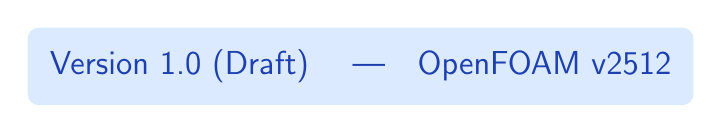
\begin{tikzpicture}
    \node[fill=primarylight, rounded corners=4pt, inner sep=8pt, font=\large\sffamily] {
	    \color{primarydark}Version 1.0 (Draft) \quad|\quad OpenFOAM v2512
    };
\end{tikzpicture}

\vspace{1.5cm}

% Feature highlights

\begin{tikzpicture}
    \node[text width=12cm, align=center, font=\normalsize\color{bodytext}] {
        \textbf{\color{primaryblue}Boundary Data Extraction} ~$\bullet$~
        \textbf{\color{secondarygreen}Time Interpolation} ~$\bullet$~
        \textbf{\color{accentpurple}Optional Encryption}
    };
\end{tikzpicture}

\vfill

% Author section
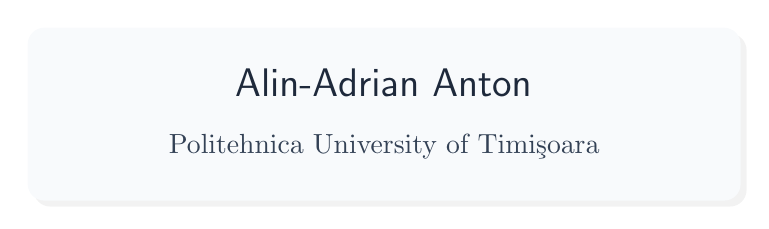
\begin{tikzpicture}
    \node[fill=codebg, rounded corners=6pt, inner sep=15pt, drop shadow=black!10] {
        \begin{minipage}{8cm}
            \centering
            {\Large\color{headingcolor}\sffamily Alin-Adrian Anton\par}
            \vspace{0.3cm}
            {\normalsize\color{bodytext} Politehnica University of Timi\c{s}oara\par}
        \end{minipage}
    };
\end{tikzpicture}

\vfill

% Date
{\color{bodytext}\sffamily Last updated: \today\par

\vspace{0.6cm}
{\footnotesize
OPENFOAM® is a registered trademark of OpenCFD Limited, producer and
distributor of the OpenFOAM software via \url{https://www.openfoam.com}.
}}

\vspace{0.8cm}

% License notice

\begin{tikzpicture}
    \node[text width=13cm, align=center, font=\footnotesize\color{codecomment}] {
        This work is licensed under CC BY-SA 4.0.\\
        \url{https://creativecommons.org/licenses/by-sa/4.0/}
    };
\end{tikzpicture}

\vspace{0.5cm}

\end{titlepage}

% ----------------------------------------------------------------------------
% COPYRIGHT AND LICENSE NOTICE
% ----------------------------------------------------------------------------

\thispagestyle{empty}
\vspace*{\fill}

\begin{center}
\begin{minipage}{0.85\textwidth}
\small

\textbf{Copyright \copyright{} 2026 Alin-Adrian Anton}

\medskip

This work is licensed under the Creative Commons Attribution-ShareAlike 4.0
International License (CC BY-SA 4.0).

\medskip

You are free to:
\begin{itemize}
    \item \textbf{Share} --- copy and redistribute the material in any medium or format
    \item \textbf{Adapt} --- remix, transform, and build upon the material for any purpose, even commercially
\end{itemize}

Under the following terms:
\begin{itemize}
    \item \textbf{Attribution} --- You must give appropriate credit, provide a link to the license, and indicate if changes were made.
    \item \textbf{ShareAlike} --- If you remix, transform, or build upon the material, you must distribute your contributions under the same license as the original.
\end{itemize}

\medskip

\url{https://creativecommons.org/licenses/by-sa/4.0/}

\end{minipage}
\end{center}

\vspace{1cm}

{\small\centering
OPENFOAM® is a registered trademark of OpenCFD Limited.\\
\centering CHERUBIM® is a registered trademark of the author. This software is libre software (libreware). 
}

\vspace*{\fill}
\newpage

% ----------------------------------------------------------------------------
% TABLE OF CONTENTS
% ----------------------------------------------------------------------------

{
\hypersetup{linkcolor=headingcolor}
\renewcommand{\contentsname}{%
    \color{primarydark}\sffamily\bfseries Contents%
}
\tableofcontents
}
\newpage

% ----------------------------------------------------------------------------
% INTRODUCTION
% ----------------------------------------------------------------------------

\section{Introduction}
\label{sec:introduction}

The \texttt{spaceTimeWindow} library enables extraction and reconstruction of spatial subsets from Large Eddy Simulation (LES) and transient RANS simulations in OpenFOAM. This technique allows researchers to:

\begin{itemize}
    \item Extract a region of interest from a full-domain simulation
    \item Store time-varying boundary conditions efficiently
    \item Reconstruct the flow within the subset using pre-computed boundary data
    \item Optionally encrypt boundary data for secure distribution
\end{itemize}

The library consists of four main components:

\begin{enumerate}
    \item \textbf{spaceTimeWindowExtract} --- Function object for boundary data extraction during simulation
    \item \textbf{spaceTimeWindowInitCase} --- Utility for reconstruction case initialization
    \item \textbf{spaceTimeWindow} --- Pure Dirichlet boundary condition for applying extracted data
    \item \textbf{spaceTimeWindowInletOutlet} --- Flux-based boundary condition (recommended for unsteady flows)
\end{enumerate}

\subsection{Requirements}

\begin{itemize}
    \item OpenFOAM v2512 (openfoam.com) or compatible ESI-OpenCFD version
    \item C++17 compatible compiler (GCC 7+ or Clang 5+)
    \item Optional: libsodium for encryption support
    \item Optional: MPI for parallel execution
\end{itemize}

\noindent
{\small OPENFOAM® is a registered trademark of OpenCFD Limited.}

\subsection{Building the Library}

\begin{lstlisting}[language=bash,caption={Building spaceTimeWindow}]
# Navigate to source directory
cd openfoam-spaceTimeWindow

# Build library and utilities
./Allwmake

# Or with encryption support (requires libsodium)
./Allwmake  # Auto-detects libsodium if installed
\end{lstlisting}

For manual building with encryption:

\begin{lstlisting}[language=bash,caption={Manual build with encryption}]
cd src/spaceTimeWindow
export FOAM_USE_SODIUM=1 && wmake

cd applications/utilities/preProcessing/spaceTimeWindowInitCase
export FOAM_USE_SODIUM=1 && wmake

cd ../spaceTimeWindowKeygen
export FOAM_USE_SODIUM=1 && wmake
\end{lstlisting}

% ----------------------------------------------------------------------------
% CONCEPT
% ----------------------------------------------------------------------------

\section{Concept: Space-Time Window Extraction and Reconstruction}
\label{sec:concept}

This section introduces the fundamental concepts behind space-time window extraction and reconstruction. Understanding these concepts is essential before diving into the technical implementation details.

\subsection{The Challenge of Large-Scale CFD Simulations}

Modern computational fluid dynamics (CFD) simulations, particularly Large Eddy Simulations (LES) and Direct Numerical Simulations (DNS), generate enormous amounts of data. A typical industrial LES simulation might involve:

\begin{itemize}
    \item Meshes with $10^7$--$10^9$ cells
    \item Thousands of timesteps
    \item Multiple field variables (velocity, pressure, turbulence quantities)
    \item Terabytes to petabytes of raw output data
\end{itemize}

Storing and post-processing this data is often impractical. The space-time window approach addresses this by extracting only the data needed to reconstruct the flow in a \emph{region of interest} at a later time.

\subsection{The Space-Time Window Concept}

A \textbf{space-time window} is a bounded region in both space (a 3D box) and time (a time interval) from which we extract the information necessary to reconstruct the flow field. The key insight is that we only need:

\begin{enumerate}
    \item \textbf{Initial conditions}: The complete field state at one timestep ($t_0$)
    \item \textbf{Boundary data}: Time-varying values on the boundary of the spatial region
\end{enumerate}

\Cref{fig:spacetime-window} illustrates this concept. The extraction box (blue) defines a spatial subset of the full domain (gray). During simulation, we record the field values on the boundary of this box at every timestep, creating a complete ``boundary history'' that can later drive a reconstruction simulation.

\begin{figure}[htbp]
\centering
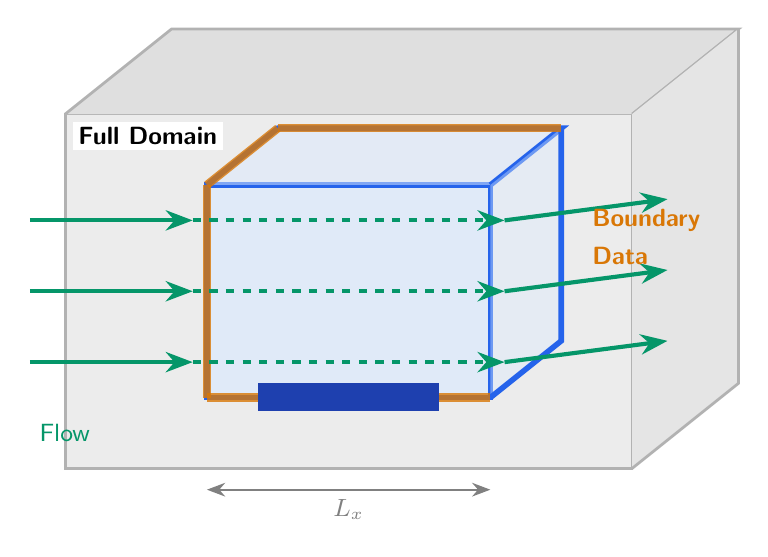
\begin{tikzpicture}[
    >=Stealth,
    scale=0.9,
    every node/.style={font=\sffamily\small}
]
    % Full domain (3D box - back faces)
    \fill[gray!15] (0,0) -- (8,0) -- (8,5) -- (0,5) -- cycle;
    \draw[gray!60, line width=1pt] (0,0) rectangle (8,5);

    % 3D effect - top face of full domain
    \fill[gray!25] (0,5) -- (1.5,6.2) -- (9.5,6.2) -- (8,5) -- cycle;
    \draw[gray!60, line width=1pt] (0,5) -- (1.5,6.2) -- (9.5,6.2) -- (8,5);

    % 3D effect - right face of full domain
    \fill[gray!20] (8,0) -- (9.5,1.2) -- (9.5,6.2) -- (8,5) -- cycle;
    \draw[gray!60, line width=1pt] (8,0) -- (9.5,1.2) -- (9.5,6.2);

    % Extraction box (smaller, inside) - front face
    \fill[primarylight, opacity=0.7] (2,1) -- (6,1) -- (6,4) -- (2,4) -- cycle;
    \draw[primaryblue, line width=2pt] (2,1) rectangle (6,4);

    % 3D effect - top face of extraction box
    \fill[primarylight, opacity=0.5] (2,4) -- (3,4.8) -- (7,4.8) -- (6,4) -- cycle;
    \draw[primaryblue, line width=2pt] (2,4) -- (3,4.8) -- (7,4.8) -- (6,4);

    % 3D effect - right face of extraction box
    \fill[primarylight, opacity=0.4] (6,1) -- (7,1.8) -- (7,4.8) -- (6,4) -- cycle;
    \draw[primaryblue, line width=2pt] (6,1) -- (7,1.8) -- (7,4.8);

    % Boundary faces highlighted (thick lines showing the "boundary data" surface)
    \draw[warningorange, line width=3pt, opacity=0.8] (2,1) -- (2,4);
    \draw[warningorange, line width=3pt, opacity=0.8] (2,1) -- (6,1);
    \draw[warningorange, line width=3pt, opacity=0.8] (2,4) -- (3,4.8);
    \draw[warningorange, line width=3pt, opacity=0.8] (3,4.8) -- (7,4.8);

    % Flow arrows (showing flow passing through)
    \foreach \y in {1.5, 2.5, 3.5} {
        \draw[->, secondarygreen, line width=1.5pt] (-0.5,\y) -- (1.8,\y);
        \draw[->, secondarygreen, line width=1.5pt, dashed] (1.8,\y) -- (6.2,\y);
        \draw[->, secondarygreen, line width=1.5pt] (6.2,\y) -- (8.5,{\y+0.3});
    }

    % Labels
    \node[anchor=north west, fill=white, inner sep=2pt] at (0.1,4.9) {\textbf{Full Domain}};
    \node[anchor=south, fill=white, inner sep=2pt, primarydark] at (4,0.8) {\textbf{Extraction Box}};
    \node[anchor=west, warningorange] at (7.3,3.5) {\textbf{Boundary}};
    \node[anchor=west, warningorange] at (7.3,3.0) {\textbf{Data}};

    % Flow direction label
    \node[secondarygreen, anchor=west] at (-0.5,0.5) {Flow};

    % Dimensions annotation
    \draw[<->, gray, line width=0.8pt] (2,-0.3) -- (6,-0.3);
    \node[gray, anchor=north] at (4,-0.3) {$L_x$};
\end{tikzpicture}
\caption{Space-time window extraction: A bounding box (blue) defines the region of interest within the full computational domain (gray). Boundary data (orange) is recorded at every timestep as the flow passes through.}
\label{fig:spacetime-window}
\end{figure}

\subsection{Extraction and Reconstruction Workflow}

The workflow consists of two distinct phases that can be separated in time and computational resources, as shown in \cref{fig:extraction-reconstruction}.

\begin{figure}[htbp]
\centering
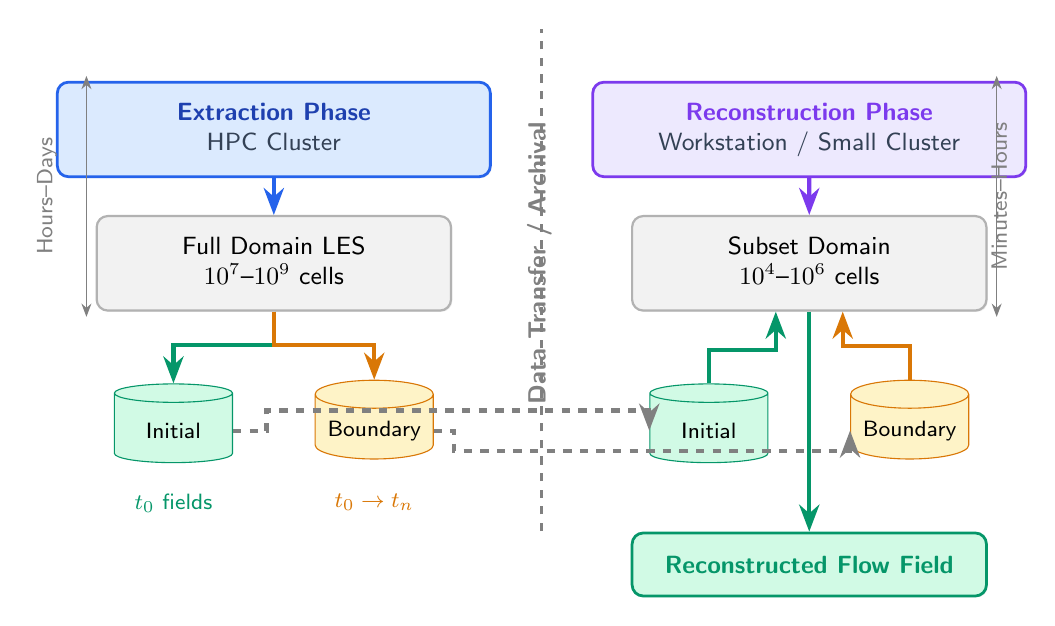
\begin{tikzpicture}[
    >=Stealth,
    scale=0.85,
    every node/.style={font=\sffamily\small},
    phase/.style={
        rectangle,
        rounded corners=4pt,
        minimum width=5.5cm,
        minimum height=1.2cm,
        text centered,
        font=\sffamily\small,
        drop shadow={shadow xshift=0.5pt, shadow yshift=-0.5pt, opacity=0.15}
    },
    data/.style={
        cylinder,
        shape border rotate=90,
        draw,
        minimum height=1cm,
        minimum width=1.5cm,
        aspect=0.25,
        font=\sffamily\footnotesize
    },
    arrow/.style={->, line width=1.5pt}
]
    % === LEFT SIDE: EXTRACTION PHASE ===
    \node[phase, fill=primarylight, draw=primaryblue, line width=1pt] (extract) at (0,4) {
        \begin{tabular}{c}
            \textbf{\color{primarydark}Extraction Phase}\\
            \color{bodytext}HPC Cluster
        \end{tabular}
    };

    % Full domain simulation
    \node[phase, fill=gray!10, draw=gray!60, line width=0.8pt, minimum width=4.5cm] (fullsim) at (0,2) {
        \begin{tabular}{c}
            Full Domain LES\\
            $10^7$--$10^9$ cells
        \end{tabular}
    };

    % Extracted data
    \node[data, fill=secondarylight, draw=secondarygreen] (initdata) at (-1.5,-0.5) {Initial};
    \node[data, fill=warninglight, draw=warningorange] (bcdata) at (1.5,-0.5) {Boundary};

    % Arrows from extraction
    \draw[arrow, primaryblue] (extract) -- (fullsim);
    \draw[arrow, secondarygreen] (fullsim.south) -- ++(0,-0.5) -| (initdata.north);
    \draw[arrow, warningorange] (fullsim.south) -- ++(0,-0.5) -| (bcdata.north);

    % Data labels
    \node[anchor=north, secondarygreen, font=\sffamily\footnotesize] at (-1.5,-1.3) {$t_0$ fields};
    \node[anchor=north, warningorange, font=\sffamily\footnotesize] at (1.5,-1.3) {$t_0 \to t_n$};

    % === STORAGE/TRANSFER ===
    \draw[dashed, gray, line width=1pt] (4,-2) -- (4,5.5);
    \node[gray, rotate=90, anchor=south] at (4.3,2) {\textbf{Data Transfer / Archival}};

    % === RIGHT SIDE: RECONSTRUCTION PHASE ===
    \node[phase, fill=accentlight, draw=accentpurple, line width=1pt] (reconstruct) at (8,4) {
        \begin{tabular}{c}
            \textbf{\color{accentpurple}Reconstruction Phase}\\
            \color{bodytext}Workstation / Small Cluster
        \end{tabular}
    };

    % Subset simulation
    \node[phase, fill=gray!10, draw=gray!60, line width=0.8pt, minimum width=4.5cm] (subsetsim) at (8,2) {
        \begin{tabular}{c}
            Subset Domain\\
            $10^4$--$10^6$ cells
        \end{tabular}
    };

    % Input data to reconstruction
    \node[data, fill=secondarylight, draw=secondarygreen] (initdata2) at (6.5,-0.5) {Initial};
    \node[data, fill=warninglight, draw=warningorange] (bcdata2) at (9.5,-0.5) {Boundary};

    % Results
    \node[phase, fill=secondarylight, draw=secondarygreen, line width=1pt, minimum width=4.5cm, minimum height=0.8cm] (results) at (8,-2.5) {
        \textbf{\color{secondarygreen}Reconstructed Flow Field}
    };

    % Arrows for reconstruction
    \draw[arrow, secondarygreen] (initdata2.north) -- ++(0,0.5) -| ([xshift=-0.5cm]subsetsim.south);
    \draw[arrow, warningorange] (bcdata2.north) -- ++(0,0.5) -| ([xshift=0.5cm]subsetsim.south);
    \draw[arrow, accentpurple] (reconstruct) -- (subsetsim);
    \draw[arrow, secondarygreen] (subsetsim.south) -- ++(0,-0.8) -- (results.north);

    % Transfer arrows
    \draw[arrow, gray, dashed] (initdata.east) -- ++(0.5,0) |- ([yshift=0.3cm]initdata2.west) -- (initdata2.west);
    \draw[arrow, gray, dashed] (bcdata.east) -- ++(0.3,0) |- ([yshift=-0.3cm]bcdata2.west) -- (bcdata2.west);

    % Time annotations
    \draw[<->, gray] (-2.8,4.8) -- (-2.8,1.2);
    \node[gray, rotate=90, anchor=south, font=\sffamily\footnotesize] at (-3.1,3) {Hours--Days};

    \draw[<->, gray] (10.8,4.8) -- (10.8,1.2);
    \node[gray, rotate=90, anchor=south, font=\sffamily\footnotesize] at (11.1,3) {Minutes--Hours};
\end{tikzpicture}
\caption{Two-phase workflow: The extraction phase runs on HPC resources and produces compact data files. The reconstruction phase can run on modest hardware, reproducing the flow in the region of interest.}
\label{fig:extraction-reconstruction}
\end{figure}

\subsubsection{Extraction Phase (HPC)}

During the original simulation on high-performance computing resources:

\begin{enumerate}
    \item The \texttt{spaceTimeWindowExtract} function object monitors the simulation
    \item At the start time ($t_0$), it extracts the complete field state within the bounding box
    \item At every timestep, it interpolates field values to the boundary faces and stores them
    \item The output is a compact dataset: initial conditions + time-varying boundary data
\end{enumerate}

\subsubsection{Reconstruction Phase (Offline)}

Later, on more modest computational resources:

\begin{enumerate}
    \item The \texttt{spaceTimeWindowInitCase} utility creates a complete simulation case
    \item The subset mesh is extracted from the original
    \item Boundary conditions are configured to read the stored boundary data
    \item The solver runs, reproducing the flow within the extraction box
\end{enumerate}

\begin{tipbox}
The reconstruction phase typically requires 100--10,000$\times$ fewer computational resources than the original simulation, making it feasible to run on a workstation or laptop.
\end{tipbox}

\subsection{Parallel Execution with MPI Domain Decomposition}
\label{sec:concept-parallel}

Large-scale CFD simulations invariably run in parallel using MPI (Message Passing Interface). The computational domain is divided among multiple processors, each handling a subset of the mesh. The spaceTimeWindow library handles both serial and parallel execution transparently.

\Cref{fig:domain-decomposition} illustrates how domain decomposition affects the extraction process. The extraction box may span multiple processor domains, requiring coordination to gather boundary data from all relevant processors.

\begin{figure}[htbp]
\centering
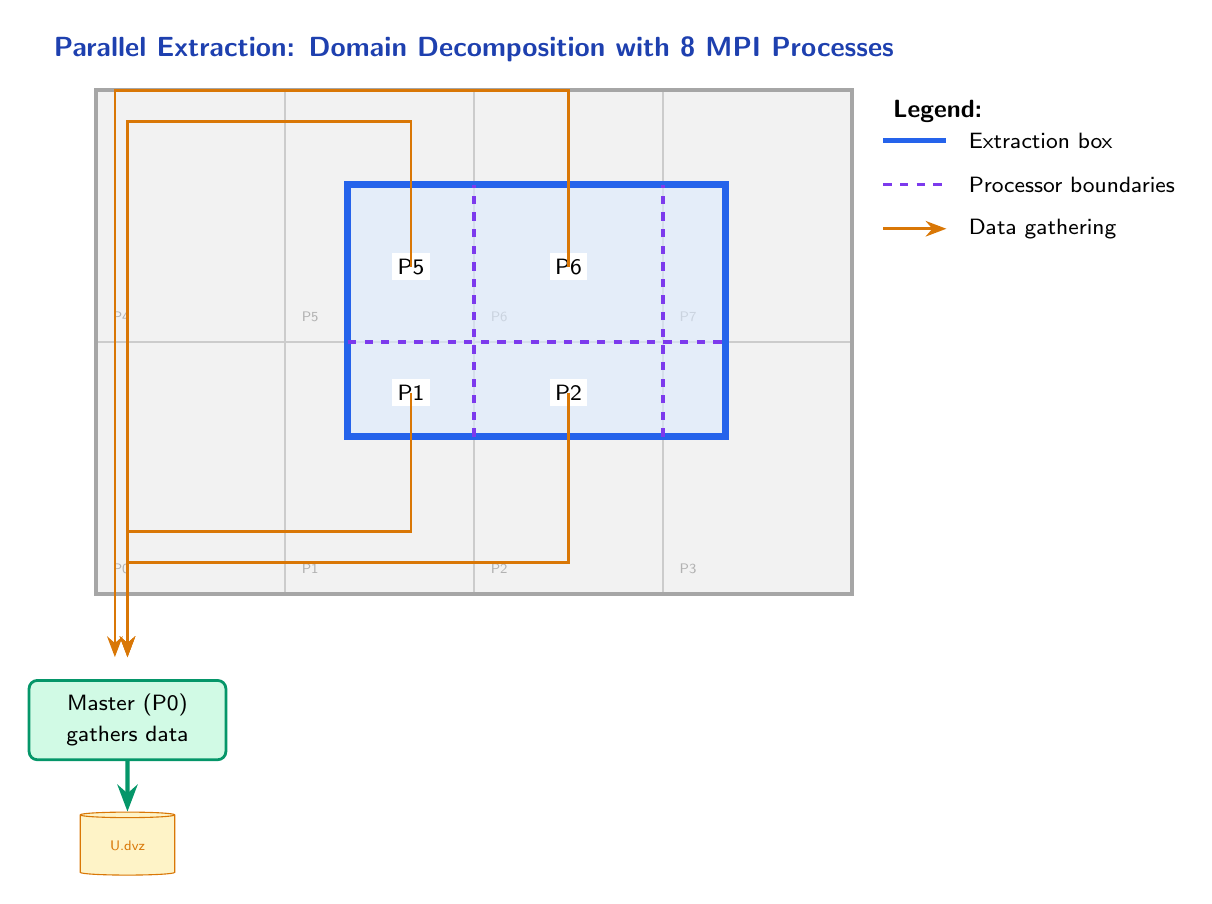
\begin{tikzpicture}[
    >=Stealth,
    scale=0.8,
    every node/.style={font=\sffamily\small}
]
    % === FULL DOMAIN WITH DECOMPOSITION ===
    % Background grid showing processor domains
    \fill[gray!10] (0,0) rectangle (12,8);

    % Processor domains (4x2 = 8 processors)
    \foreach \i in {0,1,2,3} {
        \foreach \j in {0,1} {
            \pgfmathtruncatemacro{\procnum}{\i + 4*\j}
            \draw[gray!40, line width=0.5pt] ({\i*3},{\j*4}) rectangle ({(\i+1)*3},{(\j+1)*4});
            \node[gray!60, font=\sffamily\tiny] at ({\i*3+0.4},{\j*4+0.4}) {P\procnum};
        }
    }

    % Domain outline
    \draw[gray!70, line width=1.5pt] (0,0) rectangle (12,8);

    % Extraction box spanning multiple processors
    \fill[primarylight, opacity=0.6] (4,2.5) rectangle (10,6.5);
    \draw[primaryblue, line width=2.5pt] (4,2.5) rectangle (10,6.5);

    % Highlight the processor boundaries that intersect extraction box
    \draw[accentpurple, line width=1.5pt, dashed] (6,2.5) -- (6,6.5);
    \draw[accentpurple, line width=1.5pt, dashed] (9,2.5) -- (9,6.5);
    \draw[accentpurple, line width=1.5pt, dashed] (4,4) -- (10,4);

    % Labels for processors involved
    \node[fill=white, inner sep=2pt, font=\sffamily\footnotesize] at (5,3.2) {P1};
    \node[fill=white, inner sep=2pt, font=\sffamily\footnotesize] at (7.5,3.2) {P2};
    \node[fill=white, inner sep=2pt, font=\sffamily\footnotesize] at (5,5.2) {P5};
    \node[fill=white, inner sep=2pt, font=\sffamily\footnotesize] at (7.5,5.2) {P6};

    % Arrows showing data flow to master
    \draw[->, line width=1pt, warningorange] (5,3.2) -- (5,1) -- (0.5,1) -- (0.5,-1);
    \draw[->, line width=1pt, warningorange] (7.5,3.2) -- (7.5,0.5) -- (0.5,0.5) -- (0.5,-1);
    \draw[->, line width=1pt, warningorange] (5,5.2) -- (5,7.5) -- (0.5,7.5) -- (0.5,-1);
    \draw[->, line width=1pt, warningorange] (7.5,5.2) -- (7.5,8) -- (0.3,8) -- (0.3,-1);

    % Master processor collecting data
    \node[rectangle, rounded corners=3pt, fill=secondarylight, draw=secondarygreen, line width=1pt, minimum width=2.5cm, minimum height=1cm] (master) at (0.5,-2) {
        \begin{tabular}{c}
            \footnotesize Master (P0)\\
            \footnotesize gathers data
        \end{tabular}
    };

    % Output file
    \node[cylinder, shape border rotate=90, draw=warningorange, fill=warninglight, minimum height=0.8cm, minimum width=1.2cm, aspect=0.3] (file) at (0.5,-4) {};
    \node[font=\sffamily\tiny, warningorange] at (0.5,-4) {U.dvz};

    \draw[->, line width=1.5pt, secondarygreen] (master) -- (file);

    % Legend
    \node[anchor=north west] at (12.5,8) {\textbf{Legend:}};
    \draw[primaryblue, line width=2pt] (12.5,7.2) -- (13.5,7.2);
    \node[anchor=west, font=\sffamily\footnotesize] at (13.7,7.2) {Extraction box};
    \draw[accentpurple, line width=1pt, dashed] (12.5,6.5) -- (13.5,6.5);
    \node[anchor=west, font=\sffamily\footnotesize] at (13.7,6.5) {Processor boundaries};
    \draw[->, warningorange, line width=1pt] (12.5,5.8) -- (13.5,5.8);
    \node[anchor=west, font=\sffamily\footnotesize] at (13.7,5.8) {Data gathering};

    % Title
    \node[anchor=south, font=\sffamily\bfseries, primarydark] at (6,8.3) {Parallel Extraction: Domain Decomposition with 8 MPI Processes};
\end{tikzpicture}
\caption{Domain decomposition in parallel simulations. The extraction box (blue) spans multiple processor domains. Each processor extracts its local contribution, and data is gathered to the master process for writing unified boundary data files.}
\label{fig:domain-decomposition}
\end{figure}

\subsubsection{How Parallel Extraction Works}

In parallel mode, the extraction process operates as follows:

\begin{enumerate}
    \item \textbf{Local identification}: Each processor identifies which of its cells fall within the extraction bounding box
    \item \textbf{Local extraction}: Each processor extracts field values for its local portion of the boundary
    \item \textbf{Global gathering}: Boundary data is gathered to the master processor using MPI collective operations
    \item \textbf{Unified output}: The master processor writes a single, consolidated boundary data file for each timestep
\end{enumerate}

\Cref{fig:mpi-gathering} shows the detailed data flow during the extraction process. The \texttt{spaceTimeWindowExtract} function object runs on each MPI process, extracting local contributions that are then gathered and merged into unified output files.

\begin{figure}[htbp]
\centering
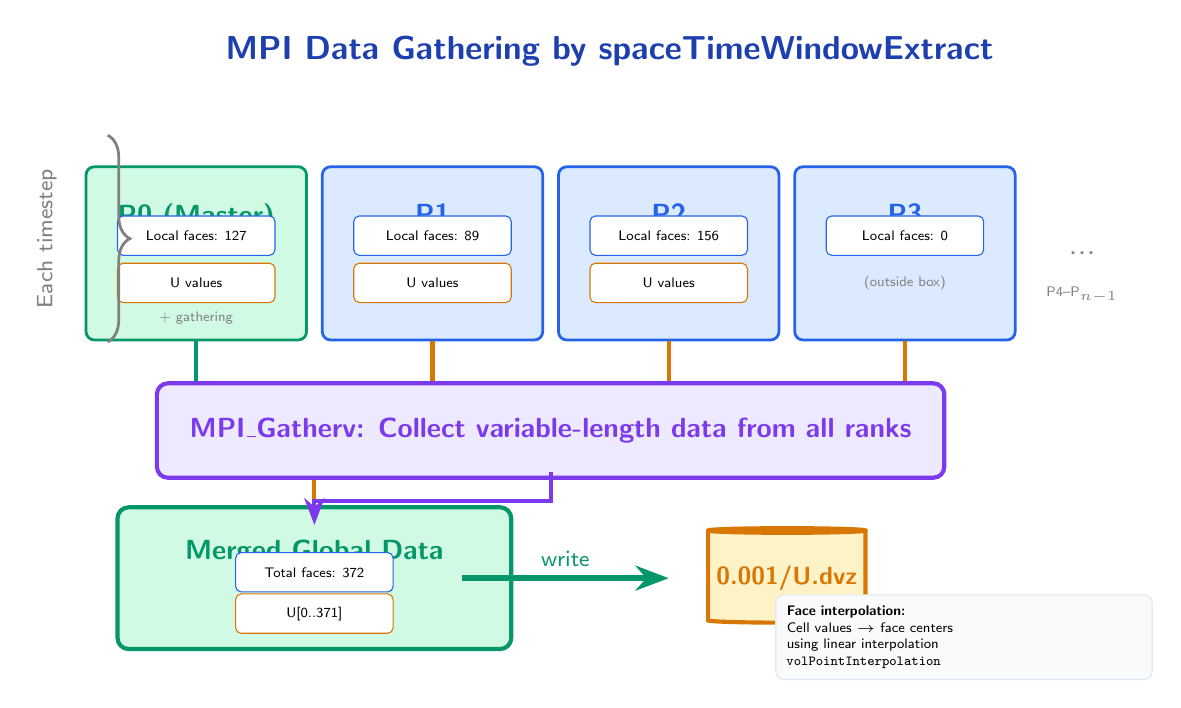
\begin{tikzpicture}[
    >=Stealth,
    scale=0.75,
    every node/.style={font=\sffamily\small},
    procbox/.style={
        rectangle,
        rounded corners=3pt,
        minimum width=2.8cm,
        minimum height=2.2cm,
        draw,
        line width=1pt
    },
    databox/.style={
        rectangle,
        rounded corners=2pt,
        minimum width=2cm,
        minimum height=0.5cm,
        draw,
        font=\sffamily\tiny
    },
    arrow/.style={->, line width=1pt}
]
    % Title
    \node[anchor=south, font=\sffamily\bfseries\large, primarydark] at (7,9) {MPI Data Gathering by spaceTimeWindowExtract};

    % === PROCESSOR BOXES (showing what each does) ===

    % P0 (Master)
    \node[procbox, fill=secondarylight, draw=secondarygreen] (p0) at (0,6) {};
    \node[anchor=north, font=\sffamily\bfseries, secondarygreen] at (0,7) {P0 (Master)};
    \node[databox, fill=white, draw=primaryblue] at (0,6.3) {Local faces: 127};
    \node[databox, fill=white, draw=warningorange] at (0,5.5) {U values};
    \node[font=\sffamily\tiny, gray] at (0,4.9) {+ gathering};

    % P1
    \node[procbox, fill=primarylight, draw=primaryblue] (p1) at (4,6) {};
    \node[anchor=north, font=\sffamily\bfseries, primaryblue] at (4,7) {P1};
    \node[databox, fill=white, draw=primaryblue] at (4,6.3) {Local faces: 89};
    \node[databox, fill=white, draw=warningorange] at (4,5.5) {U values};

    % P2
    \node[procbox, fill=primarylight, draw=primaryblue] (p2) at (8,6) {};
    \node[anchor=north, font=\sffamily\bfseries, primaryblue] at (8,7) {P2};
    \node[databox, fill=white, draw=primaryblue] at (8,6.3) {Local faces: 156};
    \node[databox, fill=white, draw=warningorange] at (8,5.5) {U values};

    % P3
    \node[procbox, fill=primarylight, draw=primaryblue] (p3) at (12,6) {};
    \node[anchor=north, font=\sffamily\bfseries, primaryblue] at (12,7) {P3};
    \node[databox, fill=white, draw=primaryblue] at (12,6.3) {Local faces: 0};
    \node[font=\sffamily\tiny, gray] at (12,5.5) {(outside box)};

    % Dots for more processors
    \node[font=\sffamily\large, gray] at (15,6) {...};
    \node[font=\sffamily\tiny, gray] at (15,5.3) {P4--P$_{n-1}$};

    % === MPI GATHER ARROWS ===
    \draw[arrow, warningorange, line width=1.5pt] (p1.south) -- ++(0,-0.8) -| (2,-0.5);
    \draw[arrow, warningorange, line width=1.5pt] (p2.south) -- ++(0,-1.2) -| (2,-0.5);
    \draw[arrow, warningorange, line width=1.5pt] (p3.south) -- ++(0,-1.6) -| (2,-0.5);
    \draw[arrow, secondarygreen, line width=1.5pt] (p0.south) -- (0,3);

    % === MPI COLLECTIVE OPERATION BOX ===
    \node[rectangle, rounded corners=4pt, fill=accentlight, draw=accentpurple, line width=1.5pt,
          minimum width=10cm, minimum height=1.2cm] (mpi) at (6,3) {};
    \node[font=\sffamily\bfseries, accentpurple] at (6,3) {MPI\_Gatherv: Collect variable-length data from all ranks};

    % === MERGED OUTPUT ===
    \node[rectangle, rounded corners=4pt, fill=secondarylight, draw=secondarygreen, line width=1.5pt,
          minimum width=5cm, minimum height=1.8cm] (merged) at (2,0.5) {};
    \node[anchor=north, font=\sffamily\bfseries, secondarygreen] at (2,1.3) {Merged Global Data};
    \node[databox, fill=white, draw=primaryblue] at (2,0.6) {Total faces: 372};
    \node[databox, fill=white, draw=warningorange] at (2,-0.1) {U[0..371]};

    % Arrow from MPI to merged
    \draw[arrow, accentpurple, line width=1.5pt] (6,2.3) -- (6,1.8) -| (2,1.4);

    % === OUTPUT FILE ===
    \node[cylinder, shape border rotate=90, draw=warningorange, fill=warninglight,
          minimum height=1.2cm, minimum width=2cm, aspect=0.25, line width=1.5pt] (file) at (10,0.5) {};
    \node[font=\sffamily\small\bfseries, warningorange] at (10,0.5) {0.001/U.dvz};

    % Arrow from merged to file
    \draw[arrow, secondarygreen, line width=2pt] (4.5,0.5) -- node[above, font=\sffamily\footnotesize] {write} (8,0.5);

    % === ANNOTATION: What happens each timestep ===
    \draw[decorate, decoration={brace, amplitude=8pt, mirror}, gray, line width=1pt]
        (-1.5,4.5) -- (-1.5,8);
    \node[gray, rotate=90, anchor=south, font=\sffamily\footnotesize] at (-2.2,6.25) {Each timestep};

    % === FACE INTERPOLATION NOTE ===
    \node[rectangle, rounded corners=3pt, fill=codebg, draw=codeframe,
          text width=4.5cm, font=\sffamily\tiny, align=left, inner sep=4pt] at (13,-0.5) {
        \textbf{Face interpolation:}\\
        Cell values $\rightarrow$ face centers\\
        using linear interpolation\\
        \texttt{volPointInterpolation}
    };
\end{tikzpicture}
\caption{Detailed MPI data gathering during parallel extraction. Each processor runs the \texttt{spaceTimeWindowExtract} function object, which identifies local boundary faces, interpolates field values to face centers, and participates in a collective gather operation. The master processor (P0) writes the merged data to a single file per timestep.}
\label{fig:mpi-gathering}
\end{figure}

This approach ensures that:
\begin{itemize}
    \item The reconstruction case is \textbf{decomposition-independent}---the same boundary data works regardless of how the original simulation was parallelized
    \item Output files are compact and self-contained, with no processor-specific information
    \item The reconstruction can run in serial or with a different parallel decomposition
\end{itemize}

\begin{notebox}
In parallel mode, mesh information is not written during extraction. Instead, the extraction box parameters are stored, and \texttt{spaceTimeWindowInitCase} creates the subset mesh from reconstructed fields. Run \texttt{reconstructPar -time <startTime>} on the source case before initializing the reconstruction case.
\end{notebox}

\subsection{Data Storage: Initial Fields and Boundary Data}
\label{sec:concept-storage}

The extracted data consists of two distinct components, illustrated in \cref{fig:data-storage}.

\begin{figure}[htbp]
\centering
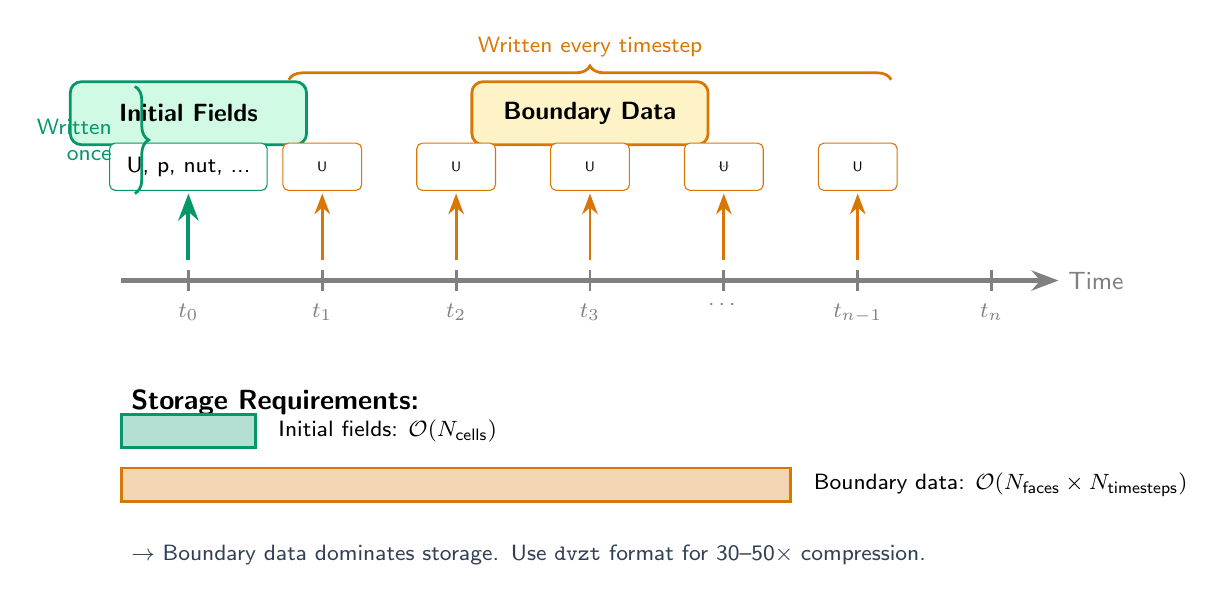
\begin{tikzpicture}[
    >=Stealth,
    scale=0.85,
    every node/.style={font=\sffamily\small},
    file/.style={
        rectangle,
        rounded corners=2pt,
        minimum width=2cm,
        minimum height=0.6cm,
        draw,
        font=\sffamily\footnotesize
    },
    folder/.style={
        rectangle,
        rounded corners=4pt,
        minimum width=3cm,
        minimum height=0.8cm,
        draw,
        line width=1pt,
        font=\sffamily\small\bfseries
    }
]
    % === TIME AXIS ===
    \draw[->, line width=1.5pt, gray] (0,0) -- (14,0);
    \node[gray, anchor=west] at (14,0) {Time};

    % Time markers
    \foreach \t/\label in {1/$t_0$, 3/$t_1$, 5/$t_2$, 7/$t_3$, 9/\ldots, 11/$t_{n-1}$, 13/$t_n$} {
        \draw[gray, line width=1pt] (\t,-0.15) -- (\t,0.15);
        \node[gray, anchor=north, font=\sffamily\footnotesize] at (\t,-0.2) {\label};
    }

    % === INITIAL FIELDS (t_0 only) ===
    \node[folder, fill=secondarylight, draw=secondarygreen] (initfolder) at (1,2.5) {Initial Fields};

    % Initial field files
    \node[file, fill=white, draw=secondarygreen] at (1,1.7) {U, p, nut, ...};

    % Arrow from t_0 to initial fields
    \draw[->, secondarygreen, line width=1.5pt] (1,0.3) -- (1,1.3);

    % Brace for "written once"
    \draw[decorate, decoration={brace, amplitude=5pt, mirror}, secondarygreen, line width=1pt]
        (0.2,1.3) -- (0.2,2.9);
    \node[secondarygreen, anchor=east, font=\sffamily\footnotesize, align=right] at (0,2.1) {Written\\once};

    % === BOUNDARY DATA (every timestep) ===
    \node[folder, fill=warninglight, draw=warningorange] (bcfolder) at (7,2.5) {Boundary Data};

    % Boundary data files for each timestep
    \foreach \x in {3, 5, 7, 9, 11} {
        \node[file, fill=white, draw=warningorange, minimum width=1cm, font=\sffamily\tiny] at (\x,1.7) {U};
    }
    \node[font=\sffamily\tiny, gray] at (9,1.7) {...};

    % Arrows from timesteps to boundary data
    \foreach \x in {3,5,7,9,11} {
        \draw[->, warningorange, line width=1pt] (\x,0.3) -- (\x,1.3);
    }

    % Brace for "written every timestep"
    \draw[decorate, decoration={brace, amplitude=5pt}, warningorange, line width=1pt]
        (2.5,3) -- (11.5,3);
    \node[warningorange, anchor=south, font=\sffamily\footnotesize] at (7,3.2) {Written every timestep};

    % === STORAGE SIZE COMPARISON ===
    \node[anchor=north west, font=\sffamily\bfseries] at (0,-1.5) {Storage Requirements:};

    % Initial fields size
    \fill[secondarygreen!30] (0,-2.5) rectangle (2,-2);
    \draw[secondarygreen, line width=1pt] (0,-2.5) rectangle (2,-2);
    \node[anchor=west, font=\sffamily\footnotesize] at (2.2,-2.25) {Initial fields: $\mathcal{O}(N_\text{cells})$};

    % Boundary data size (larger bar)
    \fill[warningorange!30] (0,-3.3) rectangle (10,-2.8);
    \draw[warningorange, line width=1pt] (0,-3.3) rectangle (10,-2.8);
    \node[anchor=west, font=\sffamily\footnotesize] at (10.2,-3.05) {Boundary data: $\mathcal{O}(N_\text{faces} \times N_\text{timesteps})$};

    % Note about compression
    \node[anchor=north west, font=\sffamily\footnotesize, text width=12cm, bodytext] at (0,-3.8) {
        $\rightarrow$ Boundary data dominates storage. Use \texttt{dvzt} format for 30--50$\times$ compression.
    };
\end{tikzpicture}
\caption{Data storage structure: Initial fields are written once at $t_0$, while boundary data is accumulated at every timestep. Compression is critical for the boundary data component.}
\label{fig:data-storage}
\end{figure}

\subsubsection{Initial Fields}

The initial fields provide the starting state for reconstruction:

\begin{itemize}
    \item \textbf{What}: Complete volumetric data (U, p, turbulence quantities) within the extraction box
    \item \textbf{When}: Written once at the extraction start time ($t_0$)
    \item \textbf{Format}: Standard OpenFOAM field format (ASCII)
    \item \textbf{Size}: Proportional to number of cells in the subset, typically megabytes
\end{itemize}

\subsubsection{Boundary Data}

The boundary data provides the time-varying boundary conditions:

\begin{itemize}
    \item \textbf{What}: Face-interpolated field values on the boundary of the extraction box
    \item \textbf{When}: Written at every timestep throughout the simulation
    \item \textbf{Format}: Configurable (ASCII, binary, or compressed \texttt{dvz}/\texttt{dvzt})
    \item \textbf{Size}: Proportional to (number of boundary faces) $\times$ (number of timesteps)
\end{itemize}

\begin{warningbox}
Boundary data accumulates rapidly during long simulations. For a typical LES with $10^4$ boundary faces and $10^4$ timesteps, uncompressed ASCII data can reach tens of gigabytes. The \texttt{dvzt} compression format reduces this by 30--50$\times$.
\end{warningbox}

\subsection{Why Reconstruction Works}
\label{sec:concept-why}

The reconstruction is possible because the governing equations (Navier-Stokes for incompressible flow) are well-posed with appropriate boundary conditions. Mathematically, if we denote:

\begin{itemize}
    \item $\Omega \subset \mathbb{R}^3$: the extraction box domain
    \item $\partial\Omega$: the boundary of the extraction box
    \item $\mathbf{u}(\mathbf{x}, t)$: the velocity field
    \item $p(\mathbf{x}, t)$: the pressure field
\end{itemize}

Then knowing $\mathbf{u}(\mathbf{x}, t_0)$ for $\mathbf{x} \in \Omega$ (initial condition) and $\mathbf{u}(\mathbf{x}, t)$ for $\mathbf{x} \in \partial\Omega$, $t \in [t_0, t_n]$ (boundary data) is sufficient to uniquely determine $\mathbf{u}(\mathbf{x}, t)$ for all $\mathbf{x} \in \Omega$, $t \in [t_0, t_n]$.

The reconstruction achieves ``bit-reproducible'' results when:
\begin{enumerate}
    \item Time interpolation is disabled (\texttt{timeInterpolationScheme none})
    \item The reconstruction runs with the same timestep as extraction
    \item The same solver settings and numerical schemes are used
\end{enumerate}

With time interpolation enabled (recommended for practical use), the reconstruction closely approximates the original solution, with errors controlled by the interpolation scheme (linear or cubic Catmull-Rom spline).

\subsection{Automatic Boundary Condition Configuration}
\label{sec:concept-auto-bc}

A key feature of the spaceTimeWindow library is the \textbf{automatic configuration} of boundary conditions during offline reconstruction. When you run \texttt{spaceTimeWindowInitCase}, the utility analyzes the extracted data and configures appropriate boundary conditions for each field---no manual setup required.

\Cref{fig:auto-bc-config} illustrates the automatic configuration process that occurs when setting up a reconstruction case on a laptop or desktop computer.

\begin{figure}[htbp]
\centering
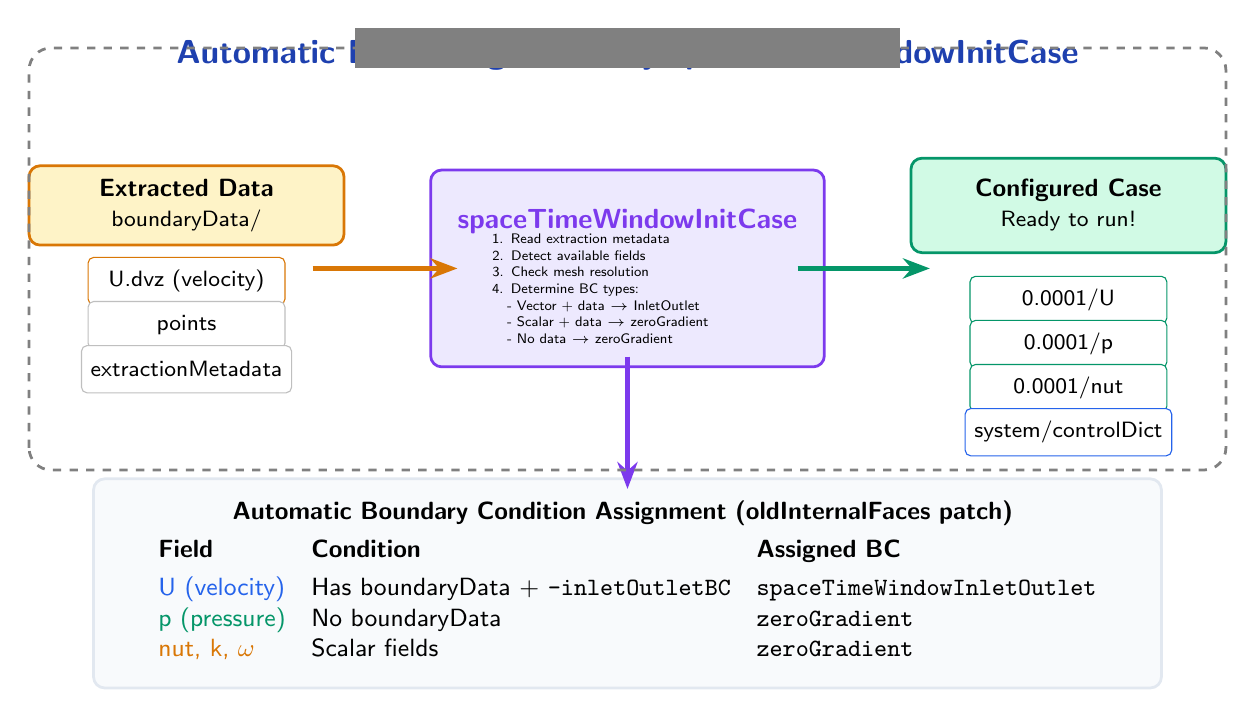
\begin{tikzpicture}[
    >=Stealth,
    scale=0.8,
    every node/.style={font=\sffamily\small},
    box/.style={
        rectangle,
        rounded corners=4pt,
        minimum width=3.5cm,
        minimum height=1cm,
        draw,
        line width=1pt,
        text centered
    },
    smallbox/.style={
        rectangle,
        rounded corners=2pt,
        minimum width=2.5cm,
        minimum height=0.6cm,
        draw,
        font=\sffamily\footnotesize
    },
    arrow/.style={->, line width=1.5pt}
]
    % Title
    \node[anchor=south, font=\sffamily\bfseries\large, primarydark] at (7,10) {Automatic BC Configuration by spaceTimeWindowInitCase};

    % === INPUT: Extracted Data ===
    \node[box, fill=warninglight, draw=warningorange, minimum width=4cm] (input) at (0,8) {
        \begin{tabular}{c}
            \textbf{Extracted Data}\\
            \footnotesize boundaryData/
        \end{tabular}
    };

    % Files in boundaryData
    \node[smallbox, fill=white, draw=warningorange] at (0,6.8) {U.dvz (velocity)};
    \node[smallbox, fill=white, draw=gray!50] at (0,6.1) {points};
    \node[smallbox, fill=white, draw=gray!50] at (0,5.4) {extractionMetadata};

    % === ANALYSIS STEP ===
    \node[box, fill=accentlight, draw=accentpurple, minimum width=5cm, minimum height=2.5cm] (analyze) at (7,7) {};
    \node[anchor=north, font=\sffamily\bfseries, accentpurple] at (7,8.1) {spaceTimeWindowInitCase};

    % Analysis steps inside
    \node[anchor=north west, font=\sffamily\tiny, text width=4.5cm, align=left] at (4.7,7.7) {
        1. Read extraction metadata\\
        2. Detect available fields\\
        3. Check mesh resolution\\
        4. Determine BC types:\\
        \quad - Vector + data $\rightarrow$ InletOutlet\\
        \quad - Scalar + data $\rightarrow$ zeroGradient\\
        \quad - No data $\rightarrow$ zeroGradient
    };

    % Arrow from input to analyze
    \draw[arrow, warningorange] (2,7) -- (4.3,7);

    % === OUTPUT: Configured Case ===
    \node[box, fill=secondarylight, draw=secondarygreen, minimum width=4cm, minimum height=1.2cm] (output) at (14,8) {
        \begin{tabular}{c}
            \textbf{Configured Case}\\
            \footnotesize Ready to run!
        \end{tabular}
    };

    % Output files
    \node[smallbox, fill=white, draw=secondarygreen] at (14,6.5) {0.0001/U};
    \node[smallbox, fill=white, draw=secondarygreen] at (14,5.8) {0.0001/p};
    \node[smallbox, fill=white, draw=secondarygreen] at (14,5.1) {0.0001/nut};
    \node[smallbox, fill=white, draw=primaryblue] at (14,4.4) {system/controlDict};

    % Arrow from analyze to output
    \draw[arrow, secondarygreen] (9.7,7) -- (11.8,7);

    % === BC DETAIL BOX ===
    \node[rectangle, rounded corners=4pt, fill=codebg, draw=codeframe, line width=1pt,
          text width=13cm, inner sep=8pt] (bcdetail) at (7,2) {
        \begin{minipage}{\linewidth}
        \centering\textbf{Automatic Boundary Condition Assignment (oldInternalFaces patch)}
        \vspace{0.3em}

        \begin{tabular}{@{}l@{\quad}l@{\quad}l@{}}
        \textbf{Field} & \textbf{Condition} & \textbf{Assigned BC} \\[0.3em]
        \textcolor{primaryblue}{U (velocity)} & Has boundaryData + \texttt{-inletOutletBC} & \texttt{spaceTimeWindowInletOutlet} \\
        \textcolor{secondarygreen}{p (pressure)} & No boundaryData & \texttt{zeroGradient} \\
        \textcolor{warningorange}{nut, k, $\omega$} & Scalar fields & \texttt{zeroGradient} \\
        \end{tabular}
        \end{minipage}
    };

    % Arrow from analyze to bcdetail
    \draw[arrow, accentpurple] (7,5.6) -- (7,3.5);

    % === USER COMPUTER CONTEXT ===
    \draw[dashed, gray, line width=1pt, rounded corners=8pt] (-2.5,3.8) rectangle (16.5,10.5);
    \node[fill=white, font=\sffamily\footnotesize, gray] at (7,10.5) {Laptop / Desktop Computer (Offline Reconstruction)};
\end{tikzpicture}
\caption{Automatic boundary condition configuration during case initialization. The \texttt{spaceTimeWindowInitCase} utility analyzes extracted data and automatically assigns appropriate boundary conditions based on field type and data availability.}
\label{fig:auto-bc-config}
\end{figure}

\subsubsection{Resolution-Independent Reconstruction}

The reconstruction can run at \textbf{different mesh resolutions} than the original extraction. This enables several important use cases:

\begin{itemize}
    \item \textbf{Coarser mesh}: Faster turnaround for exploratory analysis or debugging
    \item \textbf{Finer mesh}: Higher resolution studies without re-running the expensive global simulation
    \item \textbf{Same resolution}: Bit-reproducible reconstruction for validation
\end{itemize}

\Cref{fig:resolution-handling} shows how the \texttt{spaceTimeWindow} boundary condition automatically handles resolution differences at runtime.

\begin{figure}[htbp]
\centering
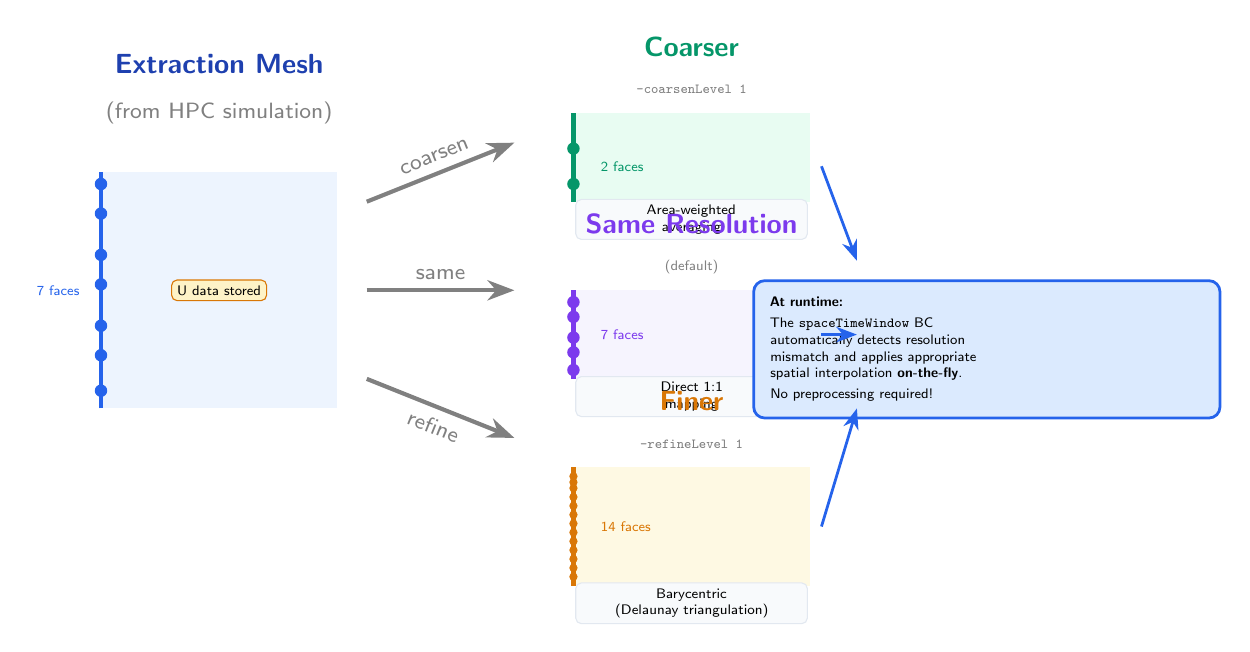
\begin{tikzpicture}[
    >=Stealth,
    scale=0.75,
    every node/.style={font=\sffamily\small},
    arrow/.style={->, line width=1.5pt}
]
    % === EXTRACTION MESH (SOURCE) ===
    \node[anchor=south, font=\sffamily\bfseries, primarydark] at (2,7.5) {Extraction Mesh};
    \node[font=\sffamily\footnotesize, gray] at (2,7) {(from HPC simulation)};

    % Draw source mesh boundary (irregular faces)
    \fill[primarylight, opacity=0.5] (0,2) rectangle (4,6);
    \draw[primaryblue, line width=1.5pt] (0,2) -- (0,6);

    % Source face points (irregular spacing)
    \foreach \y in {2.3, 2.9, 3.4, 4.1, 4.6, 5.3, 5.8} {
        \fill[primaryblue] (0,\y) circle (3pt);
    }
    \node[font=\sffamily\tiny, primaryblue, anchor=east] at (-0.2,4) {7 faces};

    % Source data indicator
    \node[rectangle, rounded corners=2pt, fill=warninglight, draw=warningorange,
          font=\sffamily\tiny, inner sep=2pt] at (2,4) {U data stored};

    % === ARROWS TO DIFFERENT RESOLUTIONS ===

    % Arrow to coarser
    \draw[arrow, gray, line width=1.5pt] (4.5,5.5) -- node[above, font=\sffamily\footnotesize, sloped] {coarsen} (7,6.5);

    % Arrow to same
    \draw[arrow, gray, line width=1.5pt] (4.5,4) -- node[above, font=\sffamily\footnotesize] {same} (7,4);

    % Arrow to finer
    \draw[arrow, gray, line width=1.5pt] (4.5,2.5) -- node[below, font=\sffamily\footnotesize, sloped] {refine} (7,1.5);

    % === COARSER RECONSTRUCTION ===
    \node[anchor=south, font=\sffamily\bfseries, secondarygreen] at (10,7.8) {Coarser};
    \node[font=\sffamily\tiny, gray] at (10,7.4) {\texttt{-coarsenLevel 1}};

    \fill[secondarylight, opacity=0.5] (8,5.5) rectangle (12,7);
    \draw[secondarygreen, line width=1.5pt] (8,5.5) -- (8,7);

    % Fewer target faces
    \foreach \y in {5.8, 6.4} {
        \fill[secondarygreen] (8,\y) circle (3pt);
    }
    \node[font=\sffamily\tiny, secondarygreen, anchor=west] at (8.3,6.1) {2 faces};

    % Interpolation method
    \node[rectangle, rounded corners=2pt, fill=codebg, draw=codeframe,
          font=\sffamily\tiny, inner sep=2pt, text width=2.8cm, align=center] at (10,5.2) {
        Area-weighted\\averaging
    };

    % === SAME RESOLUTION ===
    \node[anchor=south, font=\sffamily\bfseries, accentpurple] at (10,4.8) {Same Resolution};
    \node[font=\sffamily\tiny, gray] at (10,4.4) {(default)};

    \fill[accentlight, opacity=0.5] (8,2.5) rectangle (12,4);
    \draw[accentpurple, line width=1.5pt] (8,2.5) -- (8,4);

    % Same number of faces
    \foreach \y in {2.65, 2.95, 3.2, 3.55, 3.8} {
        \fill[accentpurple] (8,\y) circle (3pt);
    }
    \node[font=\sffamily\tiny, accentpurple, anchor=west] at (8.3,3.25) {7 faces};

    % Direct mapping
    \node[rectangle, rounded corners=2pt, fill=codebg, draw=codeframe,
          font=\sffamily\tiny, inner sep=2pt, text width=2.8cm, align=center] at (10,2.2) {
        Direct 1:1\\mapping
    };

    % === FINER RECONSTRUCTION ===
    \node[anchor=south, font=\sffamily\bfseries, warningorange] at (10,1.8) {Finer};
    \node[font=\sffamily\tiny, gray] at (10,1.4) {\texttt{-refineLevel 1}};

    \fill[warninglight, opacity=0.5] (8,-1) rectangle (12,1);
    \draw[warningorange, line width=1.5pt] (8,-1) -- (8,1);

    % More target faces
    \foreach \y in {-0.85, -0.55, -0.25, 0.05, 0.35, 0.65, 0.85} {
        \fill[warningorange] (8,\y) circle (2pt);
    }
    \foreach \y in {-0.7, -0.4, -0.1, 0.2, 0.5, 0.75} {
        \fill[warningorange] (8,\y) circle (2pt);
    }
    \node[font=\sffamily\tiny, warningorange, anchor=west] at (8.3,0) {14 faces};

    % Interpolation method
    \node[rectangle, rounded corners=2pt, fill=codebg, draw=codeframe,
          font=\sffamily\tiny, inner sep=2pt, text width=2.8cm, align=center] at (10,-1.3) {
        Barycentric\\(Delaunay triangulation)
    };

    % === RUNTIME NOTE ===
    \node[rectangle, rounded corners=4pt, fill=primarylight, draw=primaryblue, line width=1pt,
          text width=5.5cm, font=\sffamily\tiny, align=left, inner sep=6pt] at (15,3) {
        \textbf{At runtime:}\\[0.3em]
        The \texttt{spaceTimeWindow} BC\\
        automatically detects resolution\\
        mismatch and applies appropriate\\
        spatial interpolation \textbf{on-the-fly}.\\[0.3em]
        No preprocessing required!
    };

    % Arrows to runtime note
    \draw[->, primaryblue, line width=1pt] (12.2,6.1) -- (12.8,4.5);
    \draw[->, primaryblue, line width=1pt] (12.2,3.25) -- (12.8,3.25);
    \draw[->, primaryblue, line width=1pt] (12.2,0) -- (12.8,2);
\end{tikzpicture}
\caption{Resolution-independent reconstruction: The \texttt{spaceTimeWindow} boundary condition automatically handles mesh resolution differences between extraction and reconstruction. Spatial interpolation is performed on-the-fly during the simulation.}
\label{fig:resolution-handling}
\end{figure}

\subsubsection{Time Interpolation at Runtime}

Similarly, the boundary condition handles \textbf{time interpolation} automatically when the reconstruction timestep differs from the extraction timestep (which is common with adaptive timestepping). \Cref{fig:time-interpolation} illustrates the temporal interpolation process.

\begin{figure}[htbp]
\centering
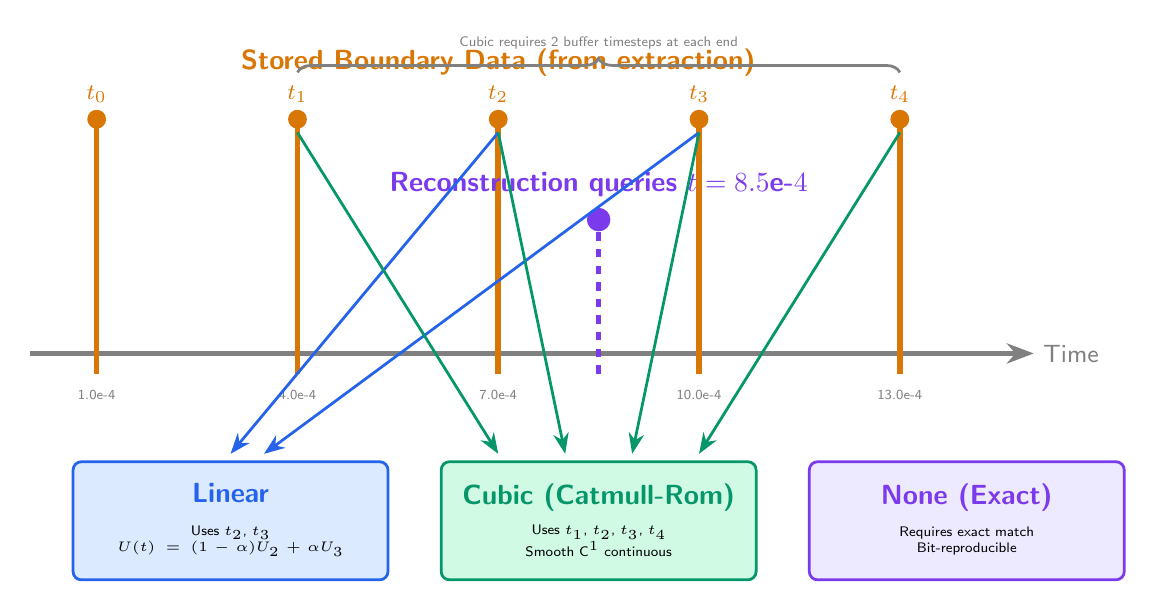
\begin{tikzpicture}[
    >=Stealth,
    scale=0.85,
    every node/.style={font=\sffamily\small}
]
    % === TIME AXIS ===
    \draw[->, line width=1.5pt, gray] (0,0) -- (15,0);
    \node[gray, anchor=west] at (15,0) {Time};

    % === EXTRACTION TIMESTEPS (stored data) ===
    \node[font=\sffamily\bfseries, warningorange, anchor=south] at (7,4) {Stored Boundary Data (from extraction)};

    \foreach \x/\label in {1/t_0, 4/t_1, 7/t_2, 10/t_3, 13/t_4} {
        \draw[warningorange, line width=2pt] (\x,-0.3) -- (\x,3.5);
        \fill[warningorange] (\x,3.5) circle (4pt);
        \node[warningorange, anchor=south, font=\sffamily\footnotesize] at (\x,3.6) {$\label$};
        \node[font=\sffamily\tiny, gray, anchor=north] at (\x,-0.4) {\x.0e-4};
    }

    % === RECONSTRUCTION QUERY TIME ===
    \node[font=\sffamily\bfseries, accentpurple, anchor=south] at (8.5,2.2) {Reconstruction queries $t = 8.5\text{e-}4$};
    \draw[accentpurple, line width=2pt, dashed] (8.5,-0.3) -- (8.5,2);
    \fill[accentpurple] (8.5,2) circle (5pt);

    % === INTERPOLATION SCHEMES ===

    % Linear interpolation
    \node[rectangle, rounded corners=3pt, fill=primarylight, draw=primaryblue, line width=1pt,
          minimum width=4cm, minimum height=1.5cm] (linear) at (3,-2.5) {};
    \node[anchor=north, font=\sffamily\bfseries, primaryblue] at (3,-1.8) {Linear};
    \node[font=\sffamily\tiny, text width=3.5cm, align=center] at (3,-2.8) {
        Uses $t_2$, $t_3$\\
        $U(t) = (1-\alpha)U_2 + \alpha U_3$
    };

    % Cubic interpolation
    \node[rectangle, rounded corners=3pt, fill=secondarylight, draw=secondarygreen, line width=1pt,
          minimum width=4cm, minimum height=1.5cm] (cubic) at (8.5,-2.5) {};
    \node[anchor=north, font=\sffamily\bfseries, secondarygreen] at (8.5,-1.8) {Cubic (Catmull-Rom)};
    \node[font=\sffamily\tiny, text width=3.5cm, align=center] at (8.5,-2.8) {
        Uses $t_1$, $t_2$, $t_3$, $t_4$\\
        Smooth C$^1$ continuous
    };

    % Exact matching
    \node[rectangle, rounded corners=3pt, fill=accentlight, draw=accentpurple, line width=1pt,
          minimum width=4cm, minimum height=1.5cm] (exact) at (14,-2.5) {};
    \node[anchor=north, font=\sffamily\bfseries, accentpurple] at (14,-1.8) {None (Exact)};
    \node[font=\sffamily\tiny, text width=3.5cm, align=center] at (14,-2.8) {
        Requires exact match\\
        Bit-reproducible
    };

    % Arrows showing which timesteps are used
    \draw[->, primaryblue, line width=1pt] (7,3.3) -- (3,-1.5);
    \draw[->, primaryblue, line width=1pt] (10,3.3) -- (3.5,-1.5);

    \draw[->, secondarygreen, line width=1pt] (4,3.3) -- (7,-1.5);
    \draw[->, secondarygreen, line width=1pt] (7,3.3) -- (8,-1.5);
    \draw[->, secondarygreen, line width=1pt] (10,3.3) -- (9,-1.5);
    \draw[->, secondarygreen, line width=1pt] (13,3.3) -- (10,-1.5);

    % Brace showing buffer requirement
    \draw[decorate, decoration={brace, amplitude=5pt}, gray, line width=1pt]
        (4,4.2) -- (13,4.2);
    \node[gray, anchor=south, font=\sffamily\tiny] at (8.5,4.4) {Cubic requires 2 buffer timesteps at each end};
\end{tikzpicture}
\caption{Time interpolation during reconstruction. When the solver requests field values at times not exactly matching stored timesteps, the boundary condition interpolates using linear (2 points) or cubic Catmull-Rom (4 points) schemes. Cubic interpolation provides smooth derivatives, essential for adaptive timestepping.}
\label{fig:time-interpolation}
\end{figure}

\begin{tipbox}
The combination of automatic spatial and temporal interpolation means you can:
\begin{itemize}
    \item Run reconstruction on a laptop with a coarser mesh for quick visualization
    \item Use adaptive timestepping (\texttt{adjustTimeStep yes}) without worrying about timestep alignment
    \item Later refine the mesh for detailed analysis without re-extracting data
\end{itemize}
All interpolation happens transparently at runtime---no preprocessing steps required.
\end{tipbox}

% ----------------------------------------------------------------------------
% ENCRYPTION
% ----------------------------------------------------------------------------

\section{Encryption of Boundary Data}
\label{sec:encryption}

The spaceTimeWindow library supports X25519 asymmetric encryption using libsodium sealed boxes. This allows secure distribution of simulation data where:

\begin{itemize}
    \item Extraction uses only the \textbf{public key}
    \item Reconstruction requires the \textbf{private key}
    \item Data cannot be decrypted without the private key
\end{itemize}

\subsection{Key Generation}

Generate a keypair using the provided utility:

\begin{lstlisting}[language=bash,caption={Generating encryption keys}]
spaceTimeWindowKeygen
# Output:
# Public key:  fqzYQ0U8j27tFEr5WzEMylbvXYP+9CAyk0JhwwZ2rwg=
# Private key: ************H8exb*****n4Kv0nu5gqljI2RPBCwl4=
#
# IMPORTANT: Store the private key securely!
\end{lstlisting}

\begin{warningbox}
The private key must be stored securely and never committed to version control. Anyone with the private key can decrypt all boundary data encrypted with the corresponding public key.
\end{warningbox}

\subsection{Secure Key Storage}

The private key should be stored using one of the following methods:

\begin{itemize}
    \item \textbf{Hardware security keys}: YubiKey, Nitrokey, or similar FIDO2/PIV-capable devices provide the strongest protection. The private key never leaves the hardware token.
    \item \textbf{Secure password managers}: KeePassXC, 1Password, Bitwarden, or similar tools with strong master passwords and optional hardware key integration.
    \item \textbf{Encrypted vaults}: GPG-encrypted files or OS keychains (macOS Keychain, GNOME Keyring, Windows Credential Manager).
\end{itemize}

\begin{tipbox}
For maximum security, generate the keypair on an air-gapped machine, store the private key on a hardware token, and only transfer the public key to the HPC system.
\end{tipbox}

\subsection{Encrypted Extraction}

Add the public key to your extraction configuration in \texttt{system/controlDict}:

\begin{lstlisting}[language=OpenFOAM,caption={Encrypted extraction configuration}]
functions
{
    extractSubset
    {
        type            spaceTimeWindowExtract;
        libs            (spaceTimeWindow);

        box             ((0.05 -0.25 0.01) (0.90 0.25 0.38));
        outputDir       "../subset-case";
        fields          (U p nut);

        writeFormat     deltaVarint;

        // Enable encryption with public key
        publicKey       "fqzYQ0U8j27tFEr5WzEMylbvXYP+9CAyk0JhwwZ2rwg=";

        writeControl    timeStep;
        writeInterval   1;
    }
}
\end{lstlisting}

Encrypted files have the \texttt{.enc} extension (e.g., \texttt{U.dvz.enc} for compressed and encrypted data).

\subsection{Decryption During Case Initialization}

When running \texttt{spaceTimeWindowInitCase} on encrypted data, you will be prompted for the private key:

\begin{lstlisting}[language=bash,caption={Decrypting boundary data}]
cd subset-case
spaceTimeWindowInitCase -sourceCase ../source-case
# Enter private key (base64): [input not echoed]
\end{lstlisting}

The utility automatically:
\begin{enumerate}
    \item Derives the public key from the private key
    \item Decrypts all \texttt{.enc} files in boundaryData
    \item Removes encrypted files after successful decryption
\end{enumerate}

\subsection{Security Properties}

\begin{itemize}
    \item \textbf{Sealed box encryption}: Anonymous sender, only recipient can decrypt
    \item \textbf{X25519 key exchange}: 128-bit security level
    \item \textbf{XSalsa20-Poly1305}: Authenticated encryption
    \item \textbf{No plaintext on disk}: Encryption occurs before writing
\end{itemize}

\subsubsection{Cryptographic Foundations}

The encryption uses elliptic curve Diffie-Hellman on Curve25519. Key generation produces a private scalar $s$ and public point (\cref{eq:pubkey}):
\begin{equation}
    P_{\text{pub}} = s \cdot G
    \label{eq:pubkey}
\end{equation}
where $G$ is the curve's base point. The discrete logarithm problem makes recovering $s$ from $P_{\text{pub}}$ computationally infeasible.

\paragraph{Sealed Box Construction}

For each encryption, a sealed box generates an ephemeral keypair $(e, e \cdot G)$ and computes a shared secret:
\begin{equation}
    K = \text{BLAKE2b}(e \cdot P_{\text{recv}}) = \text{BLAKE2b}(e \cdot s_{\text{recv}} \cdot G)
    \label{eq:shared-secret}
\end{equation}

The ciphertext is constructed as shown in \cref{eq:ciphertext}:
\begin{equation}
    C = (e \cdot G) \| \text{XSalsa20-Poly1305}_K(M)
    \label{eq:ciphertext}
\end{equation}
where $M$ is the plaintext boundary data and $\|$ denotes concatenation. The ephemeral public key $(e \cdot G)$ is prepended to allow decryption.

\paragraph{Decryption}

The recipient computes the same shared secret using their private key (\cref{eq:decrypt-key}):
\begin{equation}
    K = \text{BLAKE2b}(s_{\text{recv}} \cdot (e \cdot G))
    \label{eq:decrypt-key}
\end{equation}

By the associativity of scalar multiplication on elliptic curves (\cref{eq:key-equivalence}):
\begin{equation}
    s_{\text{recv}} \cdot (e \cdot G) = e \cdot (s_{\text{recv}} \cdot G) = e \cdot P_{\text{recv}}
    \label{eq:key-equivalence}
\end{equation}

This ensures both parties derive the same key $K$ without ever transmitting it.

\paragraph{Security Level}

X25519 provides approximately 128 bits of security. Breaking the encryption requires either:
\begin{itemize}
    \item Solving the elliptic curve discrete logarithm problem (ECDLP): $\mathcal{O}(2^{128})$ operations
    \item Brute-forcing the symmetric key: $\mathcal{O}(2^{256})$ operations for XSalsa20
\end{itemize}

\subsection{Ethical Considerations and HPC Transparency}

Most high-performance computing (HPC) centers require full transparency regarding the simulations performed on their infrastructure. For this reason, \textbf{encryption support is an optional compile-time feature} controlled by the \texttt{FOAM\_USE\_SODIUM} flag. Centers may choose not to enable this functionality.

It is important to understand what encryption does and does not protect:

\begin{itemize}
    \item \textbf{What is protected}: The time-varying boundary field data in \texttt{constant/boundaryData}. When downloaded, this data is sealed and cannot be read without the private key.

    \item \textbf{What is NOT protected}: The test case setup (mesh, dictionaries, initial conditions) remains unencrypted. Anyone can re-run the global simulation to regenerate the boundary data---encryption does not prevent this.
\end{itemize}

The practical security model relies on the following observations:

\begin{enumerate}
    \item Re-running the global simulation to obtain internal fields is \textbf{computationally expensive} and requires HPC resources. Such jobs are recorded in the scheduler logs, providing an audit trail.

    \item Offline recalculation on a personal workstation is typically infeasible due to computational cost.

    \item If file permissions on HPC scratch directories are misconfigured and the user chooses not to write timestep data from the global simulation, other users can only copy the unencrypted test case setup---not the valuable boundary data.
\end{enumerate}

\begin{notebox}
The encryption feature is designed for protecting intellectual property during data distribution, not for hiding simulations from HPC administrators. Always comply with your computing center's acceptable use policies.
\end{notebox}

\subsection{Protection Against Malware and Ransomware}

The spaceTimeWindow approach offers an additional security benefit: by storing only the minimal data required for reconstruction, the valuable simulation results can be protected against malware and ransomware attacks.

\subsubsection{Secure Archival Strategy}

The reconstruction case contains only:
\begin{itemize}
    \item The subset mesh (\texttt{constant/polyMesh})
    \item Encrypted boundary data (\texttt{constant/boundaryData/*.enc})
    \item Initial fields for one timestep
    \item Configuration dictionaries
\end{itemize}

This minimal dataset (typically a few gigabytes) can be stored on:
\begin{itemize}
    \item \textbf{Write-Once Read-Many (WORM) media}: Optical discs (M-DISC), tape archives with WORM capability, or cloud storage with object lock/immutability settings (AWS S3 Object Lock, Azure Immutable Blob Storage).
    \item \textbf{Secure vaults}: Hardware-encrypted drives kept offline, or institutional secure storage with access controls and audit logging.
    \item \textbf{Air-gapped backups}: Disconnected storage that cannot be reached by network-based malware.
\end{itemize}

\subsubsection{Security Model}

\begin{enumerate}
    \item \textbf{Encrypted boundary data is immutable}: Once written to WORM storage, the encrypted files cannot be modified or deleted by malware.
    \item \textbf{Private key stored separately}: The decryption key resides on a hardware token or secure password manager, not on the same system as the data.
    \item \textbf{Reconstruction is always possible}: Even if the HPC system or workstation is compromised, the archived data remains intact and can be decrypted on a clean system.
    \item \textbf{Minimal attack surface}: The small archive size makes backup and verification practical, unlike terabyte-scale full simulation outputs.
\end{enumerate}

\begin{tipbox}
For critical simulations, archive the encrypted reconstruction case to WORM storage immediately after extraction completes. The full simulation data can then be deleted from HPC scratch space, eliminating the risk of data loss from ransomware or accidental deletion.
\end{tipbox}

% ----------------------------------------------------------------------------
% BOUNDARY CONDITION APPROACHES
% ----------------------------------------------------------------------------

\section{Boundary Condition Approaches}
\label{sec:bc-approaches}

The library provides two approaches for applying boundary conditions on the extraction boundary (\texttt{oldInternalFaces}):

\subsection{Inlet-Outlet BC (\texttt{-inletOutletBC}) --- Recommended for Unsteady Flows}
\label{sec:inlet-outlet-bc}

Uses \texttt{spaceTimeWindowInletOutlet} BC which applies:
\begin{itemize}
    \item \textbf{Velocity (U)}: Flux-based switching --- Dirichlet (prescribed value) at inflow faces, zeroGradient at outflow faces
    \item \textbf{All scalar fields (p, nut, k, epsilon, omega)}: zeroGradient
\end{itemize}

This approach is \textbf{physically correct} for unsteady turbulent flows because:
\begin{itemize}
    \item Turbulent flows have instantaneous velocity fluctuations that can reverse direction locally
    \item Vortex shedding, recirculation zones, and turbulent eddies cause portions of the boundary to alternate between inflow and outflow
    \item Prescribing fixed values at outflow faces is non-physical (information should leave the domain freely)
    \item The flux-based switching automatically adapts to the instantaneous flow direction at each face
\end{itemize}

\begin{lstlisting}[language=bash,caption={Using inlet-outlet BC}]
spaceTimeWindowInitCase -sourceCase ../source-case -inletOutletBC
\end{lstlisting}

\subsection{Fixed Outlet Direction (\texttt{-outletDirection})}
\label{sec:fixed-outlet}

Creates a separate \texttt{outlet} patch from faces at one edge of the extraction box:
\begin{itemize}
    \item \textbf{oldInternalFaces}: Pure Dirichlet BC (\texttt{spaceTimeWindow}) on all remaining faces
    \item \textbf{outlet}: Pressure relief patch with \texttt{inletOutlet} for U and \texttt{zeroGradient} for p
\end{itemize}

Use when the mean flow direction is well-defined and outflow always occurs at a known location.

\begin{lstlisting}[language=bash,caption={Using fixed outlet direction}]
spaceTimeWindowInitCase -sourceCase ../source-case -outletDirection "(1 0 0)"
\end{lstlisting}

\begin{warningbox}
These options are mutually exclusive. Using both \texttt{-inletOutletBC} and \texttt{-outletDirection} together produces an error with guidance.
\end{warningbox}

\subsection{Boundary Condition Assignment Logic}

For each field in the initial time directory, \texttt{spaceTimeWindowInitCase} assigns BCs according to \Cref{tab:bc-assignment}.

\begin{table}[htbp]
\centering
\caption{Boundary condition assignment logic}
\label{tab:bc-assignment}
\begin{tabularx}{\textwidth}{@{}lllX@{}}
\toprule
\textbf{In boundaryData?} & \textbf{-inletOutletBC?} & \textbf{Field Type} & \textbf{BC Applied} \\
\midrule
Yes & Yes & vector (U) & \texttt{spaceTimeWindowInletOutlet} \\
Yes & Yes & scalar & \texttt{zeroGradient} \\
Yes & No & any & \texttt{spaceTimeWindow} (Dirichlet) \\
No & any & any & \texttt{zeroGradient} \\
\bottomrule
\end{tabularx}
\end{table}

This ensures fields without time-varying data automatically get appropriate BCs.

% ----------------------------------------------------------------------------
% WORKFLOW
% ----------------------------------------------------------------------------

\section{Workflow Overview}
\label{sec:workflow}

The space-time window reconstruction workflow is strictly sequential, as shown in \cref{fig:workflow}.

\begin{figure}[htbp]
\centering
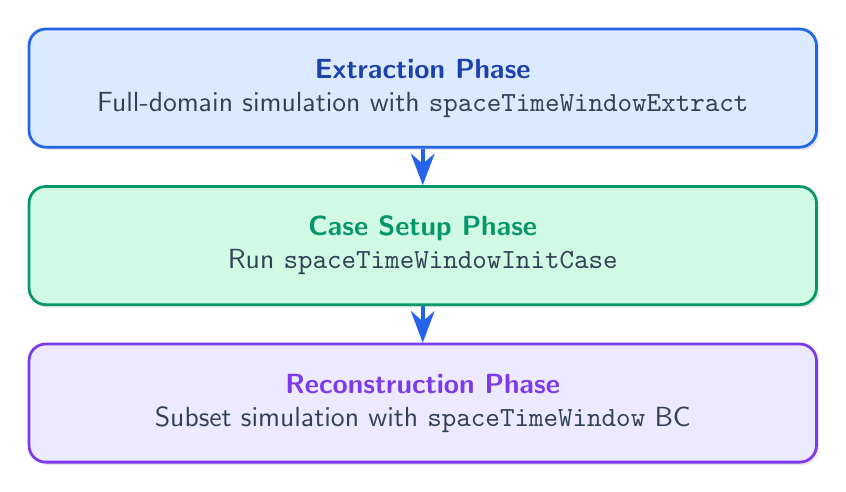
\begin{tikzpicture}[
    phase/.style={
        rectangle,
        rounded corners=6pt,
        minimum width=10cm,
        minimum height=1.5cm,
        text centered,
        font=\sffamily,
        drop shadow={shadow xshift=1pt, shadow yshift=-1pt, opacity=0.2}
    },
    arrow/.style={
        -{Stealth[length=4mm, width=3mm]},
        line width=1.5pt,
        color=primaryblue
    }
]
    % Phase 1: Extraction
    \node[phase, fill=primarylight, draw=primaryblue, line width=1pt] (phase1) at (0,4) {
        \begin{tabular}{c}
            \textbf{\color{primarydark}Extraction Phase}\\
            \color{bodytext}Full-domain simulation with \texttt{spaceTimeWindowExtract}
        \end{tabular}
    };

    % Phase 2: Setup
    \node[phase, fill=secondarylight, draw=secondarygreen, line width=1pt] (phase2) at (0,2) {
        \begin{tabular}{c}
            \textbf{\color{secondarygreen}Case Setup Phase}\\
            \color{bodytext}Run \texttt{spaceTimeWindowInitCase}
        \end{tabular}
    };

    % Phase 3: Reconstruction
    \node[phase, fill=accentlight, draw=accentpurple, line width=1pt] (phase3) at (0,0) {
        \begin{tabular}{c}
            \textbf{\color{accentpurple}Reconstruction Phase}\\
            \color{bodytext}Subset simulation with \texttt{spaceTimeWindow} BC
        \end{tabular}
    };

    % Arrows
    \draw[arrow] (phase1.south) -- (phase2.north);
    \draw[arrow] (phase2.south) -- (phase3.north);
\end{tikzpicture}
\caption{Space-time window reconstruction workflow}
\label{fig:workflow}
\end{figure}

\subsection{Serial Workflow}

\begin{lstlisting}[language=bash,caption={Complete serial workflow}]
# 1. Run extraction during simulation
cd source-case
pimpleFoam    # With spaceTimeWindowExtract function object

# 2. Initialize reconstruction case (recommended: inlet-outlet BC)
cd ../subset-case
spaceTimeWindowInitCase -sourceCase ../source-case -inletOutletBC

# 3. Run reconstruction
pimpleFoam
\end{lstlisting}

In serial mode:
\begin{itemize}
    \item Mesh and initial fields are written directly to the output directory
    \item Boundary data is written at every timestep
    \item The extractor forces field writes at $t_1$ and $t_2$ (for interpolation buffers)
\end{itemize}

\begin{notebox}
In serial mode, the extractor writes internal fields only at $t_0$ (extraction start). The $t_1$ and $t_2$ internal fields are \textbf{not} automatically saved. If you need linear interpolation starting at $t_1$, ensure your \texttt{writeInterval} captures $t_1$, or use parallel mode which forces writes at $t_0$, $t_1$, and $t_2$.
\end{notebox}

\subsection{Parallel Workflow}

\begin{enumerate}
    \item Run the original simulation in parallel with extraction enabled
    \item Run \texttt{reconstructPar} for the desired start timestep ($t_2$ for cubic interpolation)
    \item Run \texttt{spaceTimeWindowInitCase -sourceCase <path> -inletOutletBC}
    \item Run the solver on the subset case (serial or parallel)
\end{enumerate}

\begin{lstlisting}[language=bash,caption={Complete parallel workflow}]
# Step 1: Run parallel extraction
cd source-case
mpirun -np 4 pimpleFoam -parallel
# Extraction automatically forces writes at t_0, t_1, t_2

# Step 2: Reconstruct fields at cubic-safe start time (t_2)
reconstructPar -time 0.0002

# Step 3: Initialize subset case (recommended: inlet-outlet BC)
cd ../subset-case
spaceTimeWindowInitCase -sourceCase ../source-case -inletOutletBC

# Step 4: Run reconstruction
pimpleFoam
\end{lstlisting}

In parallel mode:
\begin{itemize}
    \item Boundary data from all processors is gathered to master and written as single files
    \item The extractor forces field writes at $t_0$, $t_1$, and $t_2$ for interpolation buffers ($t_0$ only in parallel)
    \item Only extraction box parameters are written (not mesh) --- \texttt{spaceTimeWindowInitCase} creates the mesh
    \item \texttt{reconstructPar} must be run at the reconstruction start time ($t_2$) to provide source fields
\end{itemize}

% ----------------------------------------------------------------------------
% CONFIGURATION FILES
% ----------------------------------------------------------------------------

\section{Configuration Reference}
\label{sec:configuration}

\subsection{Extraction Configuration}
\label{sec:config-extract}

The extraction function object is configured in \texttt{system/controlDict} within the \texttt{functions} sub-dictionary. The available parameters are listed in \cref{tab:extract-params}.

\begin{lstlisting}[language=OpenFOAM,caption={Complete extraction configuration}]
functions
{
    extractSubset
    {
        type            spaceTimeWindowExtract;
        libs            (spaceTimeWindow);

        // Bounding box: ((minX minY minZ) (maxX maxY maxZ))
        // Must be fully internal to domain
        box             ((0.05 -0.25 0.01) (0.90 0.25 0.38));

        outputDir       "../subset-case";

        // Fields for time-varying boundary data (written every timestep)
        fields          (U);              // Typically just velocity

        // Fields for initial conditions (optional, defaults to 'fields')
        initialFields   (U p nut);        // More fields for IC

        // Write format: ascii, binary, deltaVarint, or dvzt
        writeFormat     dvzt;             // Recommended: best compression

        // Precision for deltaVarint/dvzt (default: 6)
        deltaVarintPrecision  6;

        // Keyframe interval for dvzt (default: 20)
        dvztKeyframeInterval  20;

        // Gzip compression (ignored for deltaVarint/dvzt)
        writeCompression off;

        // Optional encryption
        // publicKey     "base64-encoded-public-key";

        // Time window (optional)
        // timeStart     0.0;
        // timeEnd       1.0;

        writeControl    timeStep;
        writeInterval   1;
    }
}
\end{lstlisting}

\begin{table}[htbp]
\centering
\caption{Extraction parameters}
\label{tab:extract-params}
\begin{tabularx}{\textwidth}{@{}lllX@{}}
\toprule
\textbf{Parameter} & \textbf{Type} & \textbf{Required} & \textbf{Description} \\
\midrule
\texttt{box} & pointPair & Yes & Extraction bounding box \\
\texttt{outputDir} & fileName & Yes & Output case directory \\
\texttt{fields} & wordList & Yes & Fields for time-varying BC (boundaryData) \\
\texttt{initialFields} & wordList & No & Fields for initial conditions (default: same as fields) \\
\texttt{writeFormat} & word & No & \texttt{ascii}, \texttt{binary}, \texttt{deltaVarint}, or \texttt{dvzt} \\
\texttt{deltaVarintPrecision} & label & No & Decimal digits (default: 6) \\
\texttt{dvztKeyframeInterval} & label & No & Keyframe interval for dvzt (default: 20) \\
\texttt{writeCompression} & switch & No & Gzip compression (ignored for deltaVarint/dvzt) \\
\texttt{publicKey} & string & No & Base64 public key for encryption \\
\texttt{timeStart} & scalar & No & Extraction start time \\
\texttt{timeEnd} & scalar & No & Extraction end time \\
\bottomrule
\end{tabularx}
\end{table}

\subsection{Initial Fields vs Boundary Data Fields}

The extraction can separate which fields are used for:
\begin{itemize}
    \item \textbf{Initial conditions} (\texttt{initialFields}): Fields written to the start time directory for solver initialization
    \item \textbf{Time-varying boundary data} (\texttt{fields}): Fields written to \texttt{boundaryData/} for time-varying BCs
\end{itemize}

This allows extracting more fields for initial conditions (e.g., \texttt{U p nut k omega}) while only storing time-varying data for velocity:

\begin{lstlisting}[language=OpenFOAM,caption={Field selection strategy}]
// In extraction function object
fields          (U);               // Only U for time-varying BC (saves storage)
initialFields   (U p nut);         // More fields for initial conditions
\end{lstlisting}

Fields NOT in \texttt{boundaryData} automatically get \texttt{zeroGradient} BC on \texttt{oldInternalFaces}.

\begin{tipbox}
For unsteady turbulent flows with \texttt{-inletOutletBC}, the recommended approach is to extract only velocity (\texttt{U}) for boundary data while including all turbulence fields for initial conditions. This works because pressure and turbulence quantities use zeroGradient (no BC data needed), reducing storage by approximately 66\%.
\end{tipbox}

\subsection{Boundary Condition Configuration}
\label{sec:config-bc}

\subsubsection{spaceTimeWindowInletOutlet (Recommended)}

Flux-based boundary condition that reads pre-computed velocity values and applies them only at inflow faces. The parameters are listed in \cref{tab:bc-inletoutlet-params}.

\begin{lstlisting}[language=OpenFOAM,caption={spaceTimeWindowInletOutlet configuration}]
boundaryField
{
    oldInternalFaces
    {
        type                    spaceTimeWindowInletOutlet;
        dataDir                 "constant/boundaryData";
        phi                     phi;          // Flux field name
        allowTimeInterpolation  true;
        timeInterpolationScheme cubic;        // or "linear" or "none"
        value                   uniform (0 0 0);
    }
}
\end{lstlisting}

\textbf{How it works:}
\begin{enumerate}
    \item At each timestep, reads velocity values from boundaryData (with optional time interpolation)
    \item Computes flux through each face: $\phi_f = \mathbf{U}_f \cdot \mathbf{S}_f$
    \item For inflow faces ($\phi < 0$): applies prescribed velocity from boundaryData
    \item For outflow faces ($\phi \geq 0$): applies zeroGradient (extrapolates from interior)
\end{enumerate}

\begin{table}[htbp]
\centering
\caption{spaceTimeWindowInletOutlet parameters}
\label{tab:bc-inletoutlet-params}
\begin{tabularx}{\textwidth}{@{}lllX@{}}
\toprule
\textbf{Parameter} & \textbf{Type} & \textbf{Default} & \textbf{Description} \\
\midrule
\texttt{dataDir} & fileName & \texttt{constant/boundaryData} & Path to boundary data \\
\texttt{phi} & word & \texttt{phi} & Name of flux field \\
\texttt{allowTimeInterpolation} & bool & \texttt{false} & Permit interpolation for missing timesteps \\
\texttt{timeInterpolationScheme} & word & \texttt{linear} & \texttt{none}, \texttt{linear}, or \texttt{cubic} \\
\bottomrule
\end{tabularx}
\end{table}

\subsubsection{spaceTimeWindow (Pure Dirichlet)}

Pure Dirichlet boundary condition that prescribes values on all faces regardless of flow direction. The parameters are listed in \cref{tab:bc-params}.

\begin{lstlisting}[language=OpenFOAM,caption={spaceTimeWindow configuration}]
boundaryField
{
    oldInternalFaces
    {
        type                    spaceTimeWindow;
        dataDir                 "constant/boundaryData";
        fixesValue              true;         // Tells adjustPhi these values are fixed
        allowTimeInterpolation  true;
        timeInterpolationScheme cubic;
        reportFlux              true;
        value                   uniform (0 0 0);
    }
}
\end{lstlisting}

Use this for:
\begin{itemize}
    \item Scalar fields when not using \texttt{-inletOutletBC}
    \item Situations where fixed values are explicitly desired on all faces
\end{itemize}

\begin{table}[htbp]
\centering
\caption{spaceTimeWindow parameters}
\label{tab:bc-params}
\begin{tabularx}{\textwidth}{@{}lllX@{}}
\toprule
\textbf{Parameter} & \textbf{Type} & \textbf{Default} & \textbf{Description} \\
\midrule
\texttt{dataDir} & fileName & \texttt{constant/boundaryData} & Path to boundary data \\
\texttt{fixesValue} & bool & \texttt{true} & Report to \texttt{adjustPhi} that values are fixed \\
\texttt{allowTimeInterpolation} & bool & \texttt{false} & Enable time interpolation \\
\texttt{timeInterpolationScheme} & word & \texttt{linear} & \texttt{none}, \texttt{linear}, or \texttt{cubic} \\
\texttt{reportFlux} & bool & \texttt{false} & Print net flux through patch (velocity only) \\
\texttt{setAverage} & bool & \texttt{false} & Adjust field average \\
\texttt{offset} & Type & Zero & Offset value \\
\bottomrule
\end{tabularx}
\end{table}

\subsection{Case Initialization Options}
\label{sec:config-init}

The \texttt{spaceTimeWindowInitCase} utility accepts command-line options (see \cref{tab:init-options}):

\begin{lstlisting}[language=bash,caption={spaceTimeWindowInitCase usage}]
# Recommended: inlet-outlet BC for unsteady turbulent flows
spaceTimeWindowInitCase -sourceCase ../source-case -inletOutletBC

# Alternative: fixed outlet direction for steady-mean flows
spaceTimeWindowInitCase -sourceCase ../source-case -outletDirection "(1 0 0)"

# With mass flux correction (optional, ensures exact mass conservation)
spaceTimeWindowInitCase -sourceCase ../source-case -inletOutletBC -correctMassFlux
\end{lstlisting}

\begin{table}[htbp]
\centering
\caption{spaceTimeWindowInitCase options}
\label{tab:init-options}
\begin{tabularx}{\textwidth}{@{}llX@{}}
\toprule
\textbf{Option} & \textbf{Type} & \textbf{Description} \\
\midrule
\texttt{-sourceCase} & directory & Source case where extraction ran (required) \\
\texttt{-extractDir} & directory & Directory with extracted data (default: cwd) \\
\texttt{-inletOutletBC} & flag & \textbf{Recommended.} Use flux-based inlet-outlet BC for U, zeroGradient for scalars \\
\texttt{-outletDirection} & vector & Create fixed outlet patch in given direction (e.g., ``(1 0 0)'') \\
\texttt{-outletFraction} & scalar & Fraction of box extent for outlet region (default: 0.1) \\
\texttt{-correctMassFlux} & flag & Apply least-squares mass flux correction to boundaryData \\
\texttt{-initialFields} & list & Override initial fields list (e.g., ``(U p nut k)'') \\
\texttt{-refineLevel} & label & Refine mesh N times (spatial interpolation at runtime) \\
\texttt{-coarsenLevel} & label & Coarsen mesh N times (spatial interpolation at runtime) \\
\texttt{-overwrite} & flag & Overwrite existing files \\
\bottomrule
\end{tabularx}
\end{table}

\begin{warningbox}
\texttt{-inletOutletBC} and \texttt{-outletDirection} are mutually exclusive. Using both together produces an error with guidance on which option to choose.
\end{warningbox}

\subsection{Mesh Coarsening and Refinement}
\label{sec:multiresolution}

The reconstruction mesh can be coarsened or refined relative to the extraction mesh (\cref{tab:mesh-resolution}). This enables running reconstructions at different resolutions than the original simulation.

\begin{lstlisting}[language=bash,caption={Mesh resolution options}]
# Refine mesh (finer than extraction)
spaceTimeWindowInitCase -sourceCase ../source -inletOutletBC -refineLevel 1

# Coarsen mesh (coarser than extraction)
spaceTimeWindowInitCase -sourceCase ../source -inletOutletBC -coarsenLevel 1

# Multiple levels
spaceTimeWindowInitCase -sourceCase ../source -inletOutletBC -refineLevel 2
\end{lstlisting}

\begin{table}[htbp]
\centering
\caption{Mesh resolution options}
\label{tab:mesh-resolution}
\begin{tabularx}{\textwidth}{@{}llX@{}}
\toprule
\textbf{Option} & \textbf{Type} & \textbf{Description} \\
\midrule
\texttt{-refineLevel} & label & Refine mesh N times (each level splits cells $\times 8$) \\
\texttt{-coarsenLevel} & label & Coarsen mesh N times (each level merges cells) \\
\bottomrule
\end{tabularx}
\end{table}

\begin{warningbox}
\texttt{-refineLevel} and \texttt{-coarsenLevel} are mutually exclusive. Use only one at a time.
\end{warningbox}

\subsubsection{Spatial Interpolation Algorithms}

When the reconstruction mesh differs from the extraction mesh, spatial interpolation is required for boundary data. The spaceTimeWindow boundary conditions handle this automatically at runtime using different algorithms depending on the resolution change.

\paragraph{Refinement: Barycentric Interpolation with 2D Delaunay Triangulation}

When the target mesh has more faces than the source (refinement), the algorithm triangulates source face centers using the Bowyer-Watson algorithm, as illustrated in \cref{fig:barycentric-interp}. For each target face center, the enclosing triangle is found and barycentric weights are computed. If the target point lies outside all triangles (which can happen because the extracted submesh uses original cells from the source case and may have irregular boundaries), the algorithm finds the nearest triangle by centroid distance and uses clamped barycentric coordinates. This provides smooth $C^0$ continuous interpolation.

Given a target point $\bm{p}$ inside a triangle with vertices $\bm{v}_1, \bm{v}_2, \bm{v}_3$, the barycentric coordinates $(\lambda_1, \lambda_2, \lambda_3)$ satisfy \cref{eq:barycentric-def}:
\begin{equation}
    \bm{p} = \lambda_1 \bm{v}_1 + \lambda_2 \bm{v}_2 + \lambda_3 \bm{v}_3, \quad \text{where} \quad \lambda_1 + \lambda_2 + \lambda_3 = 1
    \label{eq:barycentric-def}
\end{equation}

The weights are computed from signed triangle areas (\cref{eq:barycentric-weights}):
\begin{equation}
    \lambda_1 = \frac{A(\bm{p}, \bm{v}_2, \bm{v}_3)}{A(\bm{v}_1, \bm{v}_2, \bm{v}_3)}, \quad
    \lambda_2 = \frac{A(\bm{v}_1, \bm{p}, \bm{v}_3)}{A(\bm{v}_1, \bm{v}_2, \bm{v}_3)}, \quad
    \lambda_3 = \frac{A(\bm{v}_1, \bm{v}_2, \bm{p})}{A(\bm{v}_1, \bm{v}_2, \bm{v}_3)}
    \label{eq:barycentric-weights}
\end{equation}
where the signed area of a 2D triangle is given by \cref{eq:signed-area}:
\begin{equation}
    A(\bm{a}, \bm{b}, \bm{c}) = \frac{1}{2}\left[(b_x - a_x)(c_y - a_y) - (c_x - a_x)(b_y - a_y)\right]
    \label{eq:signed-area}
\end{equation}

The interpolated field value at the target point is then (\cref{eq:barycentric-interp}):
\begin{equation}
    \phi(\bm{p}) = \lambda_1 \phi_1 + \lambda_2 \phi_2 + \lambda_3 \phi_3
    \label{eq:barycentric-interp}
\end{equation}

\begin{figure}[htbp]
\centering
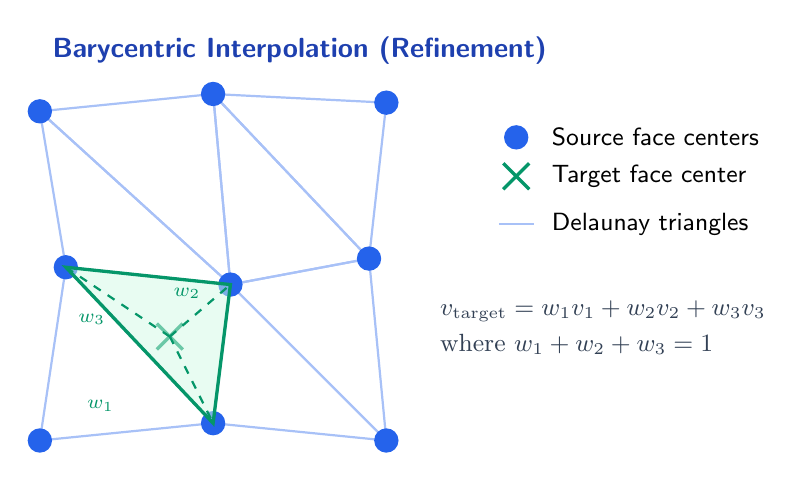
\begin{tikzpicture}[scale=1.1]
    % Title
    \node[font=\sffamily\bfseries, color=primarydark] at (3,4.5) {Barycentric Interpolation (Refinement)};

    % Source points (coarse mesh face centers) - triangulated
    \coordinate (S1) at (0,0);
    \coordinate (S2) at (2,0.2);
    \coordinate (S3) at (4,0);
    \coordinate (S4) at (0.3,2);
    \coordinate (S5) at (2.2,1.8);
    \coordinate (S6) at (3.8,2.1);
    \coordinate (S7) at (0,3.8);
    \coordinate (S8) at (2,4);
    \coordinate (S9) at (4,3.9);

    % Draw triangulation (Delaunay triangles)
    \draw[primaryblue!40, thick] (S1) -- (S2) -- (S4) -- cycle;
    \draw[primaryblue!40, thick] (S2) -- (S5) -- (S4) -- cycle;
    \draw[primaryblue!40, thick] (S2) -- (S3) -- (S5) -- cycle;
    \draw[primaryblue!40, thick] (S3) -- (S6) -- (S5) -- cycle;
    \draw[primaryblue!40, thick] (S4) -- (S5) -- (S7) -- cycle;
    \draw[primaryblue!40, thick] (S5) -- (S8) -- (S7) -- cycle;
    \draw[primaryblue!40, thick] (S5) -- (S6) -- (S8) -- cycle;
    \draw[primaryblue!40, thick] (S6) -- (S9) -- (S8) -- cycle;

    % Source points (blue circles)
    \foreach \p in {S1,S2,S3,S4,S5,S6,S7,S8,S9} {
        \fill[primaryblue] (\p) circle (4pt);
    }

    % Target point (refined mesh face center) - red X
    \coordinate (T1) at (1.5,1.2);
    \draw[secondarygreen, very thick] (T1) ++(-0.15,-0.15) -- ++(0.3,0.3);
    \draw[secondarygreen, very thick] (T1) ++(-0.15,0.15) -- ++(0.3,-0.3);

    % Highlight enclosing triangle
    \fill[secondarylight, opacity=0.5] (S2) -- (S5) -- (S4) -- cycle;
    \draw[secondarygreen, very thick] (S2) -- (S5) -- (S4) -- cycle;

    % Barycentric weight lines (dashed)
    \draw[secondarygreen, dashed, thick] (T1) -- (S2);
    \draw[secondarygreen, dashed, thick] (T1) -- (S4);
    \draw[secondarygreen, dashed, thick] (T1) -- (S5);

    % Weight labels
    \node[font=\scriptsize\sffamily, color=secondarygreen] at (0.7,0.4) {$w_1$};
    \node[font=\scriptsize\sffamily, color=secondarygreen] at (1.7,1.7) {$w_2$};
    \node[font=\scriptsize\sffamily, color=secondarygreen] at (0.6,1.4) {$w_3$};

    % Legend
    \fill[primaryblue] (5.5,3.5) circle (4pt);
    \node[right, font=\small\sffamily] at (5.8,3.5) {Source face centers};
    \draw[secondarygreen, very thick] (5.35,2.9) -- (5.65,3.2);
    \draw[secondarygreen, very thick] (5.35,3.2) -- (5.65,2.9);
    \node[right, font=\small\sffamily] at (5.8,3.05) {Target face center};
    \draw[primaryblue!40, thick] (5.3,2.5) -- (5.7,2.5);
    \node[right, font=\small\sffamily] at (5.8,2.5) {Delaunay triangles};

    % Formula
    \node[font=\small, color=bodytext, align=left] at (6.5,1.3) {$v_{\text{target}} = w_1 v_1 + w_2 v_2 + w_3 v_3$\\[2pt]where $w_1 + w_2 + w_3 = 1$};
\end{tikzpicture}
\caption{Barycentric interpolation for mesh refinement: source face centers (blue) are triangulated, and each target point (green) is interpolated using barycentric weights from the enclosing triangle}
\label{fig:barycentric-interp}
\end{figure}

\paragraph{Coarsening: Area-Weighted Averaging}

When the target mesh has fewer faces than the source (coarsening), an octree is built from source points for efficient spatial lookup, as shown in \cref{fig:area-weighted-interp}. For each target face, all source points within a search radius are found and averaged with equal weights. If no points are found, the search radius is progressively expanded. This ensures conservation of integral quantities.

For a target point $\bm{p}$ with search radius $r$, define the set of contributing source points (\cref{eq:coarsen-set}):
\begin{equation}
    \mathcal{S}(\bm{p}, r) = \left\{ i : \|\bm{x}_i - \bm{p}\| \leq r \right\}
    \label{eq:coarsen-set}
\end{equation}

The interpolated value is the arithmetic mean of all contributing sources (\cref{eq:coarsen-mean}):
\begin{equation}
    \phi(\bm{p}) = \frac{1}{|\mathcal{S}|} \sum_{i \in \mathcal{S}} \phi_i
    \label{eq:coarsen-mean}
\end{equation}

If $|\mathcal{S}| = 0$, the search radius is expanded by a factor $\alpha > 1$ (typically $\alpha = 1.5$) and the search is repeated (\cref{eq:radius-expand}):
\begin{equation}
    r \leftarrow \alpha \cdot r \quad \text{until} \quad |\mathcal{S}(\bm{p}, r)| > 0
    \label{eq:radius-expand}
\end{equation}

The octree provides $\mathcal{O}(\log N)$ lookup complexity for finding points within the search radius, making the algorithm efficient even for large meshes.

\begin{figure}[htbp]
\centering
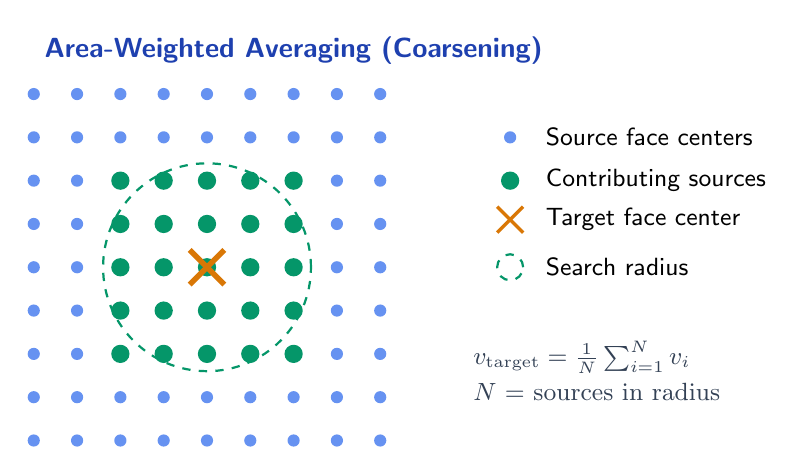
\begin{tikzpicture}[scale=1.1]
    % Title
    \node[font=\sffamily\bfseries, color=primarydark] at (3,4.5) {Area-Weighted Averaging (Coarsening)};

    % Source points (fine mesh face centers) - many points
    \foreach \x in {0,0.5,1,1.5,2,2.5,3,3.5,4} {
        \foreach \y in {0,0.5,1,1.5,2,2.5,3,3.5,4} {
            \fill[primaryblue!70] (\x,\y) circle (2pt);
        }
    }

    % Target point (coarse mesh face center)
    \coordinate (T1) at (2,2);

    % Search radius circle
    \draw[secondarygreen, thick, dashed] (T1) circle (1.2cm);

    % Highlight contributing source points
    \foreach \x in {1,1.5,2,2.5,3} {
        \foreach \y in {1,1.5,2,2.5,3} {
            \fill[secondarygreen] (\x,\y) circle (3pt);
        }
    }

    % Target point marker (large X)
    \draw[warningorange, very thick, line width=2pt] (T1) ++(-0.2,-0.2) -- ++(0.4,0.4);
    \draw[warningorange, very thick, line width=2pt] (T1) ++(-0.2,0.2) -- ++(0.4,-0.4);

    % Legend
    \fill[primaryblue!70] (5.5,3.5) circle (2pt);
    \node[right, font=\small\sffamily] at (5.8,3.5) {Source face centers};
    \fill[secondarygreen] (5.5,3.0) circle (3pt);
    \node[right, font=\small\sffamily] at (5.8,3.0) {Contributing sources};
    \draw[warningorange, very thick] (5.35,2.4) -- (5.65,2.7);
    \draw[warningorange, very thick] (5.35,2.7) -- (5.65,2.4);
    \node[right, font=\small\sffamily] at (5.8,2.55) {Target face center};
    \draw[secondarygreen, thick, dashed] (5.5,2.0) circle (0.15cm);
    \node[right, font=\small\sffamily] at (5.8,2.0) {Search radius};

    % Formula
    \node[font=\small, color=bodytext, align=left] at (6.5,0.8) {$v_{\text{target}} = \frac{1}{N}\sum_{i=1}^{N} v_i$\\[2pt]$N$ = sources in radius};
\end{tikzpicture}
\caption{Area-weighted averaging for mesh coarsening: all source face centers (blue) within the search radius of each target point (orange) are averaged with equal weights}
\label{fig:area-weighted-interp}
\end{figure}

\paragraph{2D Projection by Box Face}

The interpolation is performed on 2D point clouds, as illustrated in \cref{fig:2d-projection}. Points are grouped by which face of the extraction bounding box they belong to (6 planar surfaces: $\pm X$, $\pm Y$, $\pm Z$), then projected to 2D by dropping the constant coordinate. This exploits the box geometry while handling the irregular face distribution that arises from extracting a submesh with original cell shapes.

\begin{figure}[htbp]
\centering
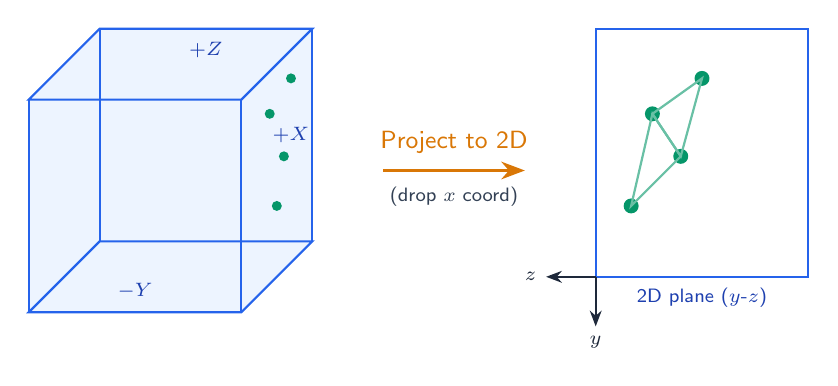
\begin{tikzpicture}[scale=0.9]
    % 3D box representation
    \coordinate (A) at (0,0);
    \coordinate (B) at (3,0);
    \coordinate (C) at (4,1);
    \coordinate (D) at (1,1);
    \coordinate (E) at (0,3);
    \coordinate (F) at (3,3);
    \coordinate (G) at (4,4);
    \coordinate (H) at (1,4);

    % Back faces (lighter)
    \fill[primarylight!50] (A) -- (B) -- (F) -- (E) -- cycle; % -Z face
    \fill[primarylight!50] (B) -- (C) -- (G) -- (F) -- cycle; % +X face
    \fill[primarylight!50] (E) -- (F) -- (G) -- (H) -- cycle; % +Y face

    % Draw edges
    \draw[primaryblue, thick] (A) -- (B) -- (C) -- (D) -- cycle; % bottom
    \draw[primaryblue, thick] (E) -- (F) -- (G) -- (H) -- cycle; % top
    \draw[primaryblue, thick] (A) -- (E);
    \draw[primaryblue, thick] (B) -- (F);
    \draw[primaryblue, thick] (C) -- (G);
    \draw[primaryblue, thick] (D) -- (H);

    % Face labels
    \node[font=\scriptsize\sffamily, color=primarydark] at (1.5,0.3) {$-Y$};
    \node[font=\scriptsize\sffamily, color=primarydark] at (3.7,2.5) {$+X$};
    \node[font=\scriptsize\sffamily, color=primarydark] at (2.5,3.7) {$+Z$};

    % Irregular face points on +X face
    \fill[secondarygreen] (3.5,1.5) circle (2pt);
    \fill[secondarygreen] (3.6,2.2) circle (2pt);
    \fill[secondarygreen] (3.4,2.8) circle (2pt);
    \fill[secondarygreen] (3.7,3.3) circle (2pt);

    % Arrow showing projection
    \draw[-{Stealth[length=3mm]}, thick, warningorange] (5,2) -- (7,2);
    \node[above, font=\small\sffamily, color=warningorange] at (6,2.1) {Project to 2D};
    \node[below, font=\scriptsize\sffamily, color=bodytext] at (6,1.9) {(drop $x$ coord)};

    % 2D projection (Y-Z plane)
    \draw[primaryblue, thick] (8,0.5) rectangle (11,4);
    \node[font=\scriptsize\sffamily, color=primarydark] at (9.5,0.2) {2D plane ($y$-$z$)};

    % Projected points
    \fill[secondarygreen] (8.5,1.5) circle (3pt);
    \fill[secondarygreen] (9.2,2.2) circle (3pt);
    \fill[secondarygreen] (8.8,2.8) circle (3pt);
    \fill[secondarygreen] (9.5,3.3) circle (3pt);

    % Triangulation in 2D
    \draw[secondarygreen!60, thick] (8.5,1.5) -- (9.2,2.2) -- (8.8,2.8) -- cycle;
    \draw[secondarygreen!60, thick] (9.2,2.2) -- (8.8,2.8) -- (9.5,3.3) -- cycle;

    % Axis labels for 2D
    \draw[-{Stealth[length=2mm]}, thick, headingcolor] (8,0.5) -- (8,-0.2);
    \node[below, font=\scriptsize\sffamily, color=headingcolor] at (8,-0.2) {$y$};
    \draw[-{Stealth[length=2mm]}, thick, headingcolor] (8,0.5) -- (7.3,0.5);
    \node[left, font=\scriptsize\sffamily, color=headingcolor] at (7.3,0.5) {$z$};
\end{tikzpicture}
\caption{Points on each box face are projected to 2D for triangulation. The constant coordinate (perpendicular to the face) is dropped, enabling efficient 2D algorithms}
\label{fig:2d-projection}
\end{figure}

\subsubsection{Initial Field Interpolation}

Initial fields are also interpolated when mesh resolution changes (see \cref{fig:mapfields-refinement,fig:volume-weighted-coarsening}):
\begin{itemize}
    \item \textbf{Refinement}: Uses \texttt{mapFields} with cell-center interpolation (\cref{fig:mapfields-refinement})
    \item \textbf{Coarsening}: Uses volume-weighted averaging of source cells (\cref{fig:volume-weighted-coarsening})
\end{itemize}

\begin{figure}[htbp]
\centering
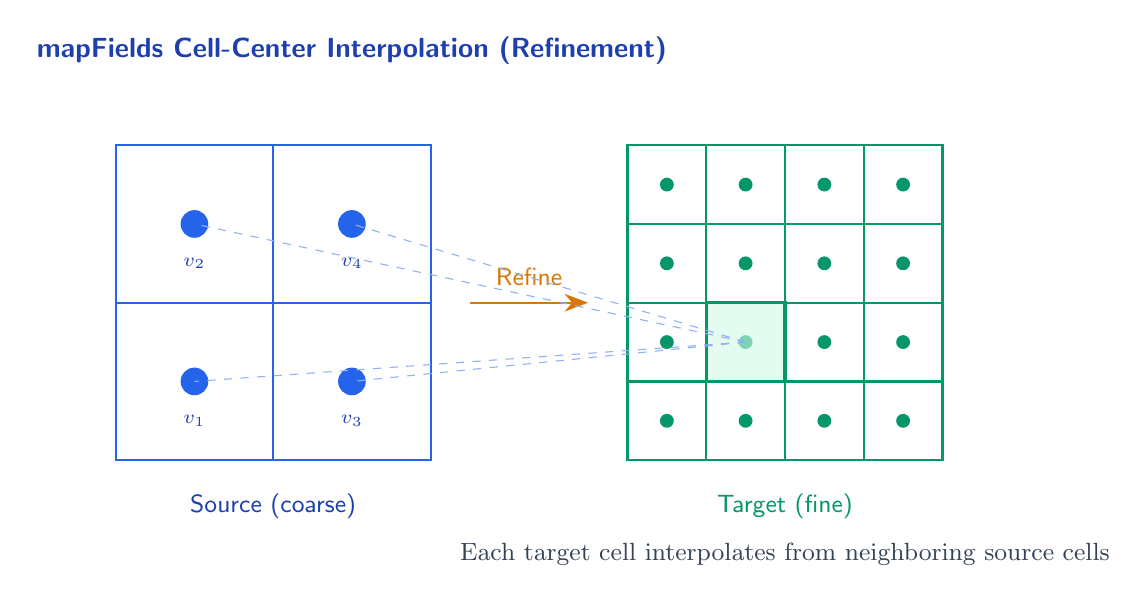
\begin{tikzpicture}[scale=1.0]
    % Title
    \node[font=\sffamily\bfseries, color=primarydark] at (3,5.2) {mapFields Cell-Center Interpolation (Refinement)};

    % Source mesh (coarse) - left side
    \draw[primaryblue, thick] (0,0) rectangle (2,4);
    \draw[primaryblue, thick] (0,2) -- (2,2);
    \draw[primaryblue, thick] (2,0) rectangle (4,4);
    \draw[primaryblue, thick] (2,2) -- (4,2);

    % Source cell centers
    \fill[primaryblue] (1,1) circle (5pt);
    \fill[primaryblue] (1,3) circle (5pt);
    \fill[primaryblue] (3,1) circle (5pt);
    \fill[primaryblue] (3,3) circle (5pt);

    % Source values labels
    \node[font=\scriptsize\sffamily, color=primarydark] at (1,0.5) {$v_1$};
    \node[font=\scriptsize\sffamily, color=primarydark] at (1,2.5) {$v_2$};
    \node[font=\scriptsize\sffamily, color=primarydark] at (3,0.5) {$v_3$};
    \node[font=\scriptsize\sffamily, color=primarydark] at (3,2.5) {$v_4$};

    % Arrow
    \draw[-{Stealth[length=3mm]}, thick, warningorange] (4.5,2) -- (6,2);
    \node[above, font=\small\sffamily, color=warningorange] at (5.25,2.1) {Refine};

    % Target mesh (fine) - right side
    \foreach \x in {6.5,7.5,8.5,9.5} {
        \foreach \y in {0,1,2,3} {
            \draw[secondarygreen, thick] (\x,\y) rectangle (\x+1,\y+1);
        }
    }

    % Target cell centers (smaller dots)
    \foreach \x in {7,8,9,10} {
        \foreach \y in {0.5,1.5,2.5,3.5} {
            \fill[secondarygreen] (\x,\y) circle (2.5pt);
        }
    }

    % Interpolation illustration - show one target cell
    \fill[secondarylight, opacity=0.6] (7.5,1) rectangle (8.5,2);
    \draw[secondarygreen, very thick] (7.5,1) rectangle (8.5,2);

    % Dashed lines to source centers showing interpolation
    \draw[primaryblue!50, dashed] (8,1.5) -- (1,1);
    \draw[primaryblue!50, dashed] (8,1.5) -- (1,3);
    \draw[primaryblue!50, dashed] (8,1.5) -- (3,1);
    \draw[primaryblue!50, dashed] (8,1.5) -- (3,3);

    % Labels
    \node[below, font=\small\sffamily, color=primarydark] at (2,-0.3) {Source (coarse)};
    \node[below, font=\small\sffamily, color=secondarygreen] at (8.5,-0.3) {Target (fine)};

    % Legend and formula
    \node[font=\small, color=bodytext, align=left] at (8.5,-1.2) {Each target cell interpolates from neighboring source cells};
\end{tikzpicture}
\caption{Initial field refinement using mapFields: target cell values are interpolated from surrounding source cell centers using distance-weighted averaging}
\label{fig:mapfields-refinement}
\end{figure}

\begin{figure}[htbp]
\centering
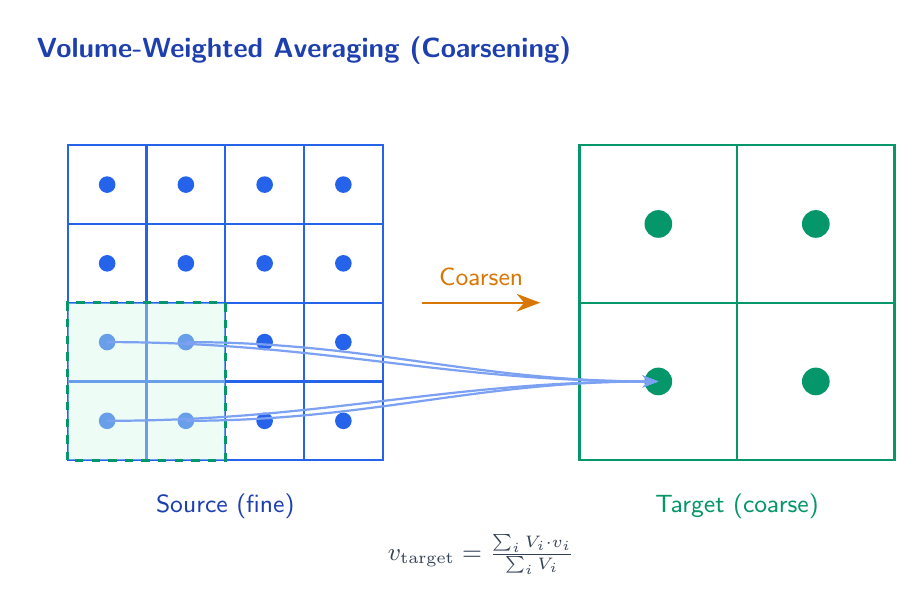
\begin{tikzpicture}[scale=1.0]
    % Title
    \node[font=\sffamily\bfseries, color=primarydark] at (3,5.2) {Volume-Weighted Averaging (Coarsening)};

    % Source mesh (fine) - left side
    \foreach \x in {0,1,2,3} {
        \foreach \y in {0,1,2,3} {
            \draw[primaryblue, thick] (\x,\y) rectangle (\x+1,\y+1);
        }
    }

    % Source cell centers with values
    \foreach \x in {0.5,1.5,2.5,3.5} {
        \foreach \y in {0.5,1.5,2.5,3.5} {
            \fill[primaryblue] (\x,\y) circle (3pt);
        }
    }

    % Highlight a group that will be averaged
    \fill[secondarylight, opacity=0.4] (0,0) rectangle (2,2);
    \draw[secondarygreen, very thick, dashed] (0,0) rectangle (2,2);

    % Arrow
    \draw[-{Stealth[length=3mm]}, thick, warningorange] (4.5,2) -- (6,2);
    \node[above, font=\small\sffamily, color=warningorange] at (5.25,2.1) {Coarsen};

    % Target mesh (coarse) - right side
    \draw[secondarygreen, thick] (6.5,0) rectangle (8.5,4);
    \draw[secondarygreen, thick] (6.5,2) -- (8.5,2);
    \draw[secondarygreen, thick] (8.5,0) rectangle (10.5,4);
    \draw[secondarygreen, thick] (8.5,2) -- (10.5,2);

    % Target cell centers
    \fill[secondarygreen] (7.5,1) circle (5pt);
    \fill[secondarygreen] (7.5,3) circle (5pt);
    \fill[secondarygreen] (9.5,1) circle (5pt);
    \fill[secondarygreen] (9.5,3) circle (5pt);

    % Show averaging arrows from source to target
    \draw[primaryblue!60, thick, -{Stealth[length=2mm]}] (0.5,0.5) to[out=0,in=180] (7.5,1);
    \draw[primaryblue!60, thick, -{Stealth[length=2mm]}] (1.5,0.5) to[out=0,in=180] (7.5,1);
    \draw[primaryblue!60, thick, -{Stealth[length=2mm]}] (0.5,1.5) to[out=0,in=180] (7.5,1);
    \draw[primaryblue!60, thick, -{Stealth[length=2mm]}] (1.5,1.5) to[out=0,in=180] (7.5,1);

    % Labels
    \node[below, font=\small\sffamily, color=primarydark] at (2,-0.3) {Source (fine)};
    \node[below, font=\small\sffamily, color=secondarygreen] at (8.5,-0.3) {Target (coarse)};

    % Formula
    \node[font=\small, color=bodytext, align=center] at (5.25,-1.2) {$v_{\text{target}} = \frac{\sum_i V_i \cdot v_i}{\sum_i V_i}$};
\end{tikzpicture}
\caption{Initial field coarsening using volume-weighted averaging: source cell values within each target cell region are averaged weighted by their volumes}
\label{fig:volume-weighted-coarsening}
\end{figure}

\begin{notebox}
Spatial interpolation introduces smoothing, particularly for coarsening. For turbulent flows, this may affect small-scale structures. Consider the trade-off between computational cost and resolution fidelity.
\end{notebox}

\textbf{What spaceTimeWindowInitCase creates:}

\begin{enumerate}
    \item \texttt{system/controlDict} --- With matching solver, deltaT, adjustTimeStep from extraction
    \begin{itemize}
        \item \texttt{startTime} set to $t_2$ (third timestep) for cubic interpolation buffer
        \item \texttt{endTime} set to $t_{n-2}$ (third-to-last) for cubic interpolation buffer
    \end{itemize}
    \item \texttt{system/fvSchemes}, \texttt{system/fvSolution} --- Copied from source case (with pRefPoint added)
    \item \texttt{constant/} files --- All physics properties copied (mandatory for fidelity)
    \item Initial field files with appropriate BCs based on options and boundaryData availability
\end{enumerate}

% ----------------------------------------------------------------------------
% DATA STORAGE
% ----------------------------------------------------------------------------

\section{Data Storage Format}
\label{sec:storage}

\subsection{Directory Structure}

The extraction creates the following directory structure:

\begin{lstlisting}[language=bash,caption={Extracted data structure}]
outputDir/
    constant/
        polyMesh/               # Subset mesh
            points
            faces
            owner
            neighbour
            boundary
            extractionBox       # (parallel only)
        boundaryData/
            oldInternalFaces/
                points              # Face centres
                extractionMetadata  # Settings and timestep list
                0.0001/
                    U               # or U.dvz or U.dvz.enc
                    p
                    nut
                0.0002/
                    ...
    0.0001/                     # Initial fields (serial only)
        U
        p
        nut
\end{lstlisting}

\subsection{Boundary Data Compression}

The \texttt{writeFormat} parameter controls how boundary data files are written, with compression ratios summarized in \cref{tab:compression}.

\begin{table}[htbp]
\centering
\caption{Compression comparison}
\label{tab:compression}
\begin{tabular}{@{}llll@{}}
\toprule
\textbf{Format} & \textbf{Extension} & \textbf{Typical Size} & \textbf{Notes} \\
\midrule
ASCII & (none) & 100\% & Human-readable \\
Binary & (none) & $\sim$50\% & OpenFOAM native \\
ASCII + gzip & .gz & $\sim$10\% & Compressed \\
Binary + gzip & .gz & $\sim$8\% & Compressed \\
deltaVarint & .dvz & $\sim$2.7\% & High compression, self-contained \\
dvzt & .dvzt & $\sim$2.4\% & Best compression, recommended \\
\bottomrule
\end{tabular}
\end{table}

\subsubsection{Delta-Varint Codec (DVZ)}

Specialized codec optimized for CFD boundary data (see \cref{fig:dvz-pipeline,fig:spatial-delta}):

\begin{enumerate}
    \item \textbf{Component-major ordering}: Groups similar values (all $U_x$, then $U_y$, then $U_z$)
    \item \textbf{Spatial delta encoding}: Stores differences between consecutive face values within the same timestep
    \item \textbf{Quantization}: Rounds to configurable precision
    \item \textbf{Varint encoding}: Variable-length integer encoding
    \item \textbf{Zigzag encoding}: Efficient signed integer representation
\end{enumerate}

\begin{figure}[htbp]
\centering
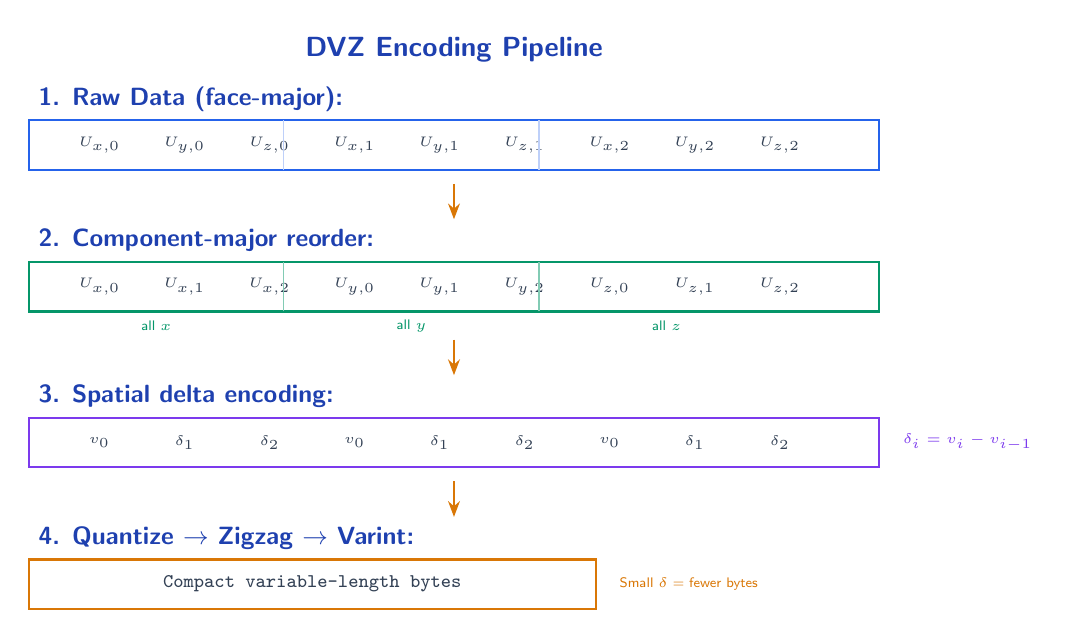
\begin{tikzpicture}[scale=0.9]
    % Title
    \node[font=\sffamily\bfseries, color=primarydark] at (6,6.5) {DVZ Encoding Pipeline};

    % Step 1: Raw data (row-major)
    \node[font=\small\sffamily\bfseries, color=primarydark, anchor=west] at (0,5.8) {1. Raw Data (face-major):};
    \draw[primaryblue, thick] (0,4.8) rectangle (12,5.5);
    \foreach \x/\label in {0.6/$U_{x,0}$, 1.8/$U_{y,0}$, 3.0/$U_{z,0}$, 4.2/$U_{x,1}$, 5.4/$U_{y,1}$, 6.6/$U_{z,1}$, 7.8/$U_{x,2}$, 9.0/$U_{y,2}$, 10.2/$U_{z,2}$} {
        \node[font=\tiny\ttfamily, color=bodytext] at (\x+0.4,5.15) {\label};
    }
    \draw[primaryblue!30] (3.6,4.8) -- (3.6,5.5);
    \draw[primaryblue!30] (7.2,4.8) -- (7.2,5.5);

    % Arrow
    \draw[-{Stealth[length=2mm]}, thick, warningorange] (6,4.6) -- (6,4.1);

    % Step 2: Component-major reordering
    \node[font=\small\sffamily\bfseries, color=primarydark, anchor=west] at (0,3.8) {2. Component-major reorder:};
    \draw[secondarygreen, thick] (0,2.8) rectangle (12,3.5);
    \foreach \x/\label in {0.6/$U_{x,0}$, 1.8/$U_{x,1}$, 3.0/$U_{x,2}$, 4.2/$U_{y,0}$, 5.4/$U_{y,1}$, 6.6/$U_{y,2}$, 7.8/$U_{z,0}$, 9.0/$U_{z,1}$, 10.2/$U_{z,2}$} {
        \node[font=\tiny\ttfamily, color=bodytext] at (\x+0.4,3.15) {\label};
    }
    \draw[secondarygreen!50] (3.6,2.8) -- (3.6,3.5);
    \draw[secondarygreen!50] (7.2,2.8) -- (7.2,3.5);
    \node[font=\tiny\sffamily, color=secondarygreen] at (1.8,2.6) {all $x$};
    \node[font=\tiny\sffamily, color=secondarygreen] at (5.4,2.6) {all $y$};
    \node[font=\tiny\sffamily, color=secondarygreen] at (9.0,2.6) {all $z$};

    % Arrow
    \draw[-{Stealth[length=2mm]}, thick, warningorange] (6,2.4) -- (6,1.9);

    % Step 3: Delta encoding
    \node[font=\small\sffamily\bfseries, color=primarydark, anchor=west] at (0,1.6) {3. Spatial delta encoding:};
    \draw[accentpurple, thick] (0,0.6) rectangle (12,1.3);
    \foreach \x/\label in {0.6/$v_0$, 1.8/$\delta_1$, 3.0/$\delta_2$, 4.2/$v_0$, 5.4/$\delta_1$, 6.6/$\delta_2$, 7.8/$v_0$, 9.0/$\delta_1$, 10.2/$\delta_2$} {
        \node[font=\tiny\ttfamily, color=bodytext] at (\x+0.4,0.95) {\label};
    }
    \node[font=\tiny\sffamily, color=accentpurple, anchor=west] at (12.2,0.95) {$\delta_i = v_i - v_{i-1}$};

    % Arrow
    \draw[-{Stealth[length=2mm]}, thick, warningorange] (6,0.4) -- (6,-0.1);

    % Step 4: Quantize + Zigzag + Varint
    \node[font=\small\sffamily\bfseries, color=primarydark, anchor=west] at (0,-0.4) {4. Quantize $\rightarrow$ Zigzag $\rightarrow$ Varint:};
    \draw[warningorange, thick] (0,-1.4) rectangle (8,-0.7);
    \node[font=\scriptsize\ttfamily, color=bodytext] at (4,-1.05) {Compact variable-length bytes};
    \node[font=\tiny\sffamily, color=warningorange, anchor=west] at (8.2,-1.05) {Small $\delta$ = fewer bytes};
\end{tikzpicture}
\caption{DVZ encoding pipeline: data is reordered by component for better locality, then delta-encoded spatially. Quantization, zigzag encoding (for signed integers), and variable-length integer encoding produce compact output}
\label{fig:dvz-pipeline}
\end{figure}

\begin{figure}[htbp]
\centering
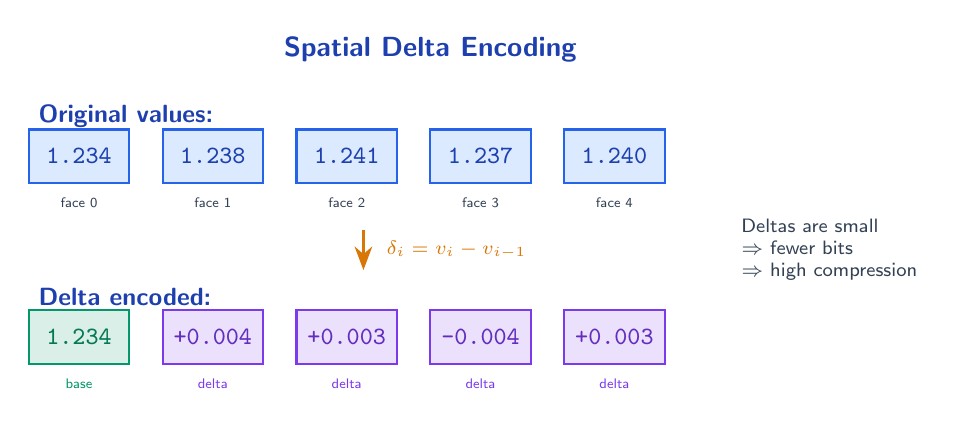
\begin{tikzpicture}[scale=0.85]
    % Title
    \node[font=\sffamily\bfseries, color=primarydark] at (6,5.5) {Spatial Delta Encoding};

    % Original values
    \node[font=\small\sffamily\bfseries, color=primarydark, anchor=west] at (0,4.5) {Original values:};

    % Face boxes with values
    \foreach \x/\val in {0/1.234, 2/1.238, 4/1.241, 6/1.237, 8/1.240} {
        \draw[primaryblue, thick, fill=primarylight] (\x,3.5) rectangle (\x+1.5,4.3);
        \node[font=\small\ttfamily, color=primarydark] at (\x+0.75,3.9) {\val};
    }
    \node[font=\tiny\sffamily, color=bodytext] at (0.75,3.2) {face 0};
    \node[font=\tiny\sffamily, color=bodytext] at (2.75,3.2) {face 1};
    \node[font=\tiny\sffamily, color=bodytext] at (4.75,3.2) {face 2};
    \node[font=\tiny\sffamily, color=bodytext] at (6.75,3.2) {face 3};
    \node[font=\tiny\sffamily, color=bodytext] at (8.75,3.2) {face 4};

    % Arrow
    \draw[-{Stealth[length=3mm]}, thick, warningorange] (5,2.8) -- (5,2.2);
    \node[right, font=\scriptsize\sffamily, color=warningorange] at (5.2,2.5) {$\delta_i = v_i - v_{i-1}$};

    % Delta values
    \node[font=\small\sffamily\bfseries, color=primarydark, anchor=west] at (0,1.8) {Delta encoded:};

    \foreach \x/\val/\col in {0/1.234/secondarygreen, 2/+0.004/accentpurple, 4/+0.003/accentpurple, 6/-0.004/accentpurple, 8/+0.003/accentpurple} {
        \draw[\col, thick, fill=\col!15] (\x,0.8) rectangle (\x+1.5,1.6);
        \node[font=\small\ttfamily, color=\col!80!black] at (\x+0.75,1.2) {\val};
    }
    \node[font=\tiny\sffamily, color=secondarygreen] at (0.75,0.5) {base};
    \node[font=\tiny\sffamily, color=accentpurple] at (2.75,0.5) {delta};
    \node[font=\tiny\sffamily, color=accentpurple] at (4.75,0.5) {delta};
    \node[font=\tiny\sffamily, color=accentpurple] at (6.75,0.5) {delta};
    \node[font=\tiny\sffamily, color=accentpurple] at (8.75,0.5) {delta};

    % Compression benefit note
    \node[font=\scriptsize\sffamily, color=bodytext, align=left, anchor=west] at (10.5,2.5) {Deltas are small\\$\Rightarrow$ fewer bits\\$\Rightarrow$ high compression};
\end{tikzpicture}
\caption{Spatial delta encoding: instead of storing absolute values, DVZ stores the first value and differences between consecutive faces. Smooth CFD fields have small deltas, enabling high compression}
\label{fig:spatial-delta}
\end{figure}

\begin{notebox}
Each DVZ timestep file is completely self-contained. Delta encoding is purely spatial (between consecutive faces in a single field), not temporal. Any timestep can be read independently without access to other timesteps.
\end{notebox}

\subsubsection{DVZ Mathematical Formulation}

\paragraph{Component-Major Reordering}

For a vector field $\bm{U}$ with $N$ faces, the raw data layout is face-major (\cref{eq:dvz-raw}):
\begin{equation}
    \text{Raw}: [U_{x,0}, U_{y,0}, U_{z,0}, U_{x,1}, U_{y,1}, U_{z,1}, \ldots, U_{x,N-1}, U_{y,N-1}, U_{z,N-1}]
    \label{eq:dvz-raw}
\end{equation}

DVZ reorders to component-major for better compression (\cref{eq:dvz-reorder}):
\begin{equation}
    \text{Reordered}: [\underbrace{U_{x,0}, U_{x,1}, \ldots, U_{x,N-1}}_{\text{all } x}, \underbrace{U_{y,0}, \ldots, U_{y,N-1}}_{\text{all } y}, \underbrace{U_{z,0}, \ldots, U_{z,N-1}}_{\text{all } z}]
    \label{eq:dvz-reorder}
\end{equation}

\paragraph{Spatial Delta Encoding}

For each component sequence $\{v_0, v_1, \ldots, v_{N-1}\}$, store deltas as shown in \cref{eq:dvz-delta}:
\begin{equation}
    \delta_0 = v_0, \quad \delta_i = v_i - v_{i-1} \quad \text{for } i = 1, \ldots, N-1
    \label{eq:dvz-delta}
\end{equation}

For smooth CFD fields, consecutive face values are similar, so $|\delta_i| \ll |v_i|$.

\paragraph{Quantization}

Convert floating-point deltas to integers with configurable precision $p$ (decimal digits) using \cref{eq:dvz-quantize}:
\begin{equation}
    q_i = \text{round}(\delta_i \times 10^p)
    \label{eq:dvz-quantize}
\end{equation}

The precision parameter controls the trade-off between compression ratio and accuracy. With $p = 6$ (default), values are accurate to $\sim 10^{-6}$ relative precision.

\paragraph{Zigzag Encoding}

Convert signed integers to unsigned for efficient varint encoding (\cref{eq:dvz-zigzag}):
\begin{equation}
    z_i = \begin{cases}
        2q_i & \text{if } q_i \geq 0 \\
        -2q_i - 1 & \text{if } q_i < 0
    \end{cases}
    = (q_i \ll 1) \oplus (q_i \gg 31)
    \label{eq:dvz-zigzag}
\end{equation}

This maps small-magnitude signed integers to small unsigned integers: $0 \mapsto 0$, $-1 \mapsto 1$, $1 \mapsto 2$, $-2 \mapsto 3$, etc.

\paragraph{Variable-Length Integer Encoding}

Encode unsigned integers using 7 bits per byte, with the high bit indicating continuation (\cref{eq:dvz-varint}):
\begin{equation}
    \text{bytes}(z) = \left\lceil \frac{\lfloor \log_2(z) \rfloor + 1}{7} \right\rceil
    \label{eq:dvz-varint}
\end{equation}

Small values ($z < 128$) use 1 byte; larger values use more bytes. Since smooth CFD fields produce small deltas, most values compress to 1--2 bytes instead of 4--8 bytes for raw floats/doubles.

\subsubsection{Delta-Varint-Temporal Codec (DVZT)}

Enhanced codec that exploits both spatial and temporal correlation for better compression (see \cref{fig:dvzt-structure,fig:dvzt-prediction,fig:dvzt-workflow}):

\begin{enumerate}
    \item \textbf{Keyframes} (every N timesteps): Self-contained, same as DVZ (\cref{fig:dvzt-structure})
    \item \textbf{Delta frames}: Hybrid spatial-temporal prediction (\cref{fig:dvzt-prediction})
    \begin{itemize}
        \item Uses weighted prediction: $\hat{v} = 0.3 \cdot v_{\text{spatial}} + 0.7 \cdot v_{\text{temporal}}$
        \item Encodes residuals (actual - predicted) instead of raw spatial deltas
        \item Typically $\sim$10\% smaller than DVZ for delta frames
    \end{itemize}
\end{enumerate}

\begin{figure}[htbp]
\centering
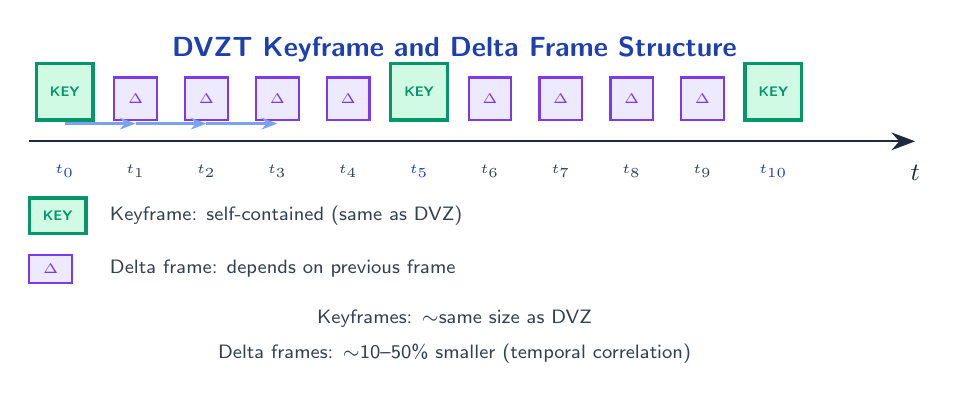
\begin{tikzpicture}[scale=0.9]
    % Title
    \node[font=\sffamily\bfseries, color=primarydark] at (6,5.8) {DVZT Keyframe and Delta Frame Structure};

    % Timeline
    \draw[-{Stealth[length=3mm]}, thick, headingcolor] (0,4.5) -- (12.5,4.5);
    \node[below, font=\small\sffamily, color=headingcolor] at (12.5,4.3) {$t$};

    % Keyframes (every 5 for illustration)
    \foreach \x/\t in {0.5/$t_0$, 5.5/$t_5$, 10.5/$t_{10}$} {
        \draw[secondarygreen, very thick, fill=secondarylight] (\x-0.4,4.8) rectangle (\x+0.4,5.6);
        \node[font=\tiny\sffamily\bfseries, color=secondarygreen] at (\x,5.2) {KEY};
        \node[below, font=\tiny\sffamily, color=primarydark] at (\x,4.3) {\t};
    }

    % Delta frames
    \foreach \x/\t in {1.5/$t_1$, 2.5/$t_2$, 3.5/$t_3$, 4.5/$t_4$, 6.5/$t_6$, 7.5/$t_7$, 8.5/$t_8$, 9.5/$t_9$} {
        \draw[accentpurple, thick, fill=accentlight] (\x-0.3,4.8) rectangle (\x+0.3,5.4);
        \node[font=\tiny\sffamily, color=accentpurple] at (\x,5.1) {$\Delta$};
        \node[below, font=\tiny\sffamily, color=bodytext] at (\x,4.3) {\t};
    }

    % Dependency arrows
    \draw[-{Stealth[length=2mm]}, thick, primaryblue!60] (0.5,4.75) -- (1.5,4.75);
    \draw[-{Stealth[length=2mm]}, thick, primaryblue!60] (1.5,4.75) -- (2.5,4.75);
    \draw[-{Stealth[length=2mm]}, thick, primaryblue!60] (2.5,4.75) -- (3.5,4.75);

    % Legend
    \draw[secondarygreen, very thick, fill=secondarylight] (0,3.2) rectangle (0.8,3.7);
    \node[font=\tiny\sffamily\bfseries, color=secondarygreen] at (0.4,3.45) {KEY};
    \node[right, font=\scriptsize\sffamily, color=bodytext] at (1,3.45) {Keyframe: self-contained (same as DVZ)};

    \draw[accentpurple, thick, fill=accentlight] (0,2.5) rectangle (0.6,2.9);
    \node[font=\tiny\sffamily, color=accentpurple] at (0.3,2.7) {$\Delta$};
    \node[right, font=\scriptsize\sffamily, color=bodytext] at (1,2.7) {Delta frame: depends on previous frame};

    % Size comparison
    \node[font=\scriptsize\sffamily, color=bodytext, align=left] at (6,2.0) {Keyframes: $\sim$same size as DVZ};
    \node[font=\scriptsize\sffamily, color=bodytext, align=left] at (6,1.5) {Delta frames: $\sim$10--50\% smaller (temporal correlation)};
\end{tikzpicture}
\caption{DVZT frame structure: keyframes are self-contained and appear every N timesteps (configurable). Delta frames between keyframes use temporal prediction for better compression}
\label{fig:dvzt-structure}
\end{figure}

\begin{figure}[htbp]
\centering
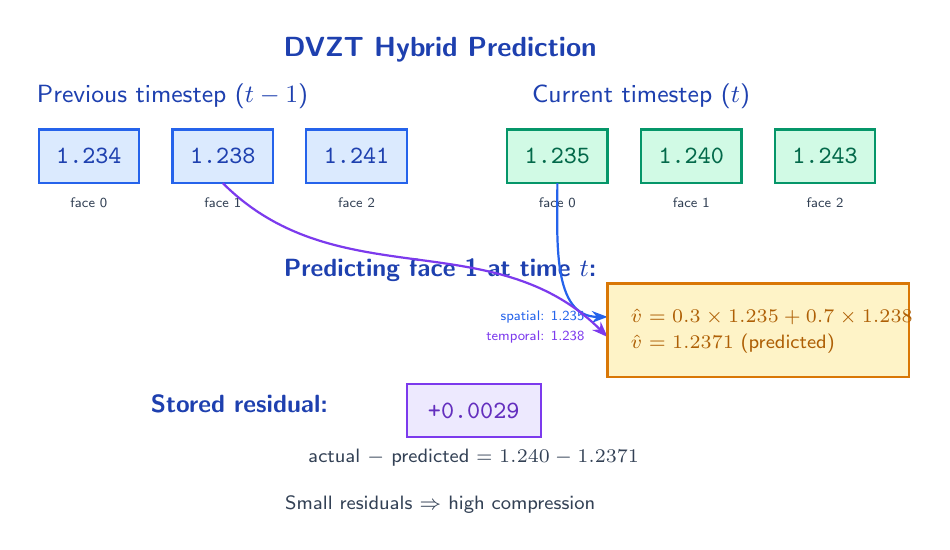
\begin{tikzpicture}[scale=0.85]
    % Title
    \node[font=\sffamily\bfseries, color=primarydark] at (6,6.5) {DVZT Hybrid Prediction};

    % Time labels
    \node[font=\small\sffamily, color=primarydark] at (2,5.8) {Previous timestep ($t-1$)};
    \node[font=\small\sffamily, color=primarydark] at (9,5.8) {Current timestep ($t$)};

    % Previous timestep faces
    \foreach \x/\val in {0/1.234, 2/1.238, 4/1.241} {
        \draw[primaryblue, thick, fill=primarylight] (\x,4.5) rectangle (\x+1.5,5.3);
        \node[font=\small\ttfamily, color=primarydark] at (\x+0.75,4.9) {\val};
    }
    \node[font=\tiny\sffamily, color=bodytext] at (0.75,4.2) {face 0};
    \node[font=\tiny\sffamily, color=bodytext] at (2.75,4.2) {face 1};
    \node[font=\tiny\sffamily, color=bodytext] at (4.75,4.2) {face 2};

    % Current timestep faces
    \foreach \x/\val in {7/1.235, 9/1.240, 11/1.243} {
        \draw[secondarygreen, thick, fill=secondarylight] (\x,4.5) rectangle (\x+1.5,5.3);
        \node[font=\small\ttfamily, color=secondarygreen!70!black] at (\x+0.75,4.9) {\val};
    }
    \node[font=\tiny\sffamily, color=bodytext] at (7.75,4.2) {face 0};
    \node[font=\tiny\sffamily, color=bodytext] at (9.75,4.2) {face 1};
    \node[font=\tiny\sffamily, color=bodytext] at (11.75,4.2) {face 2};

    % Prediction for face 1
    \node[font=\small\sffamily\bfseries, color=primarydark] at (6,3.2) {Predicting face 1 at time $t$:};

    % Spatial neighbor arrow
    \draw[-{Stealth[length=2mm]}, thick, primaryblue] (7.75,4.5) to[out=-90,in=180] (8.5,2.5);
    \node[font=\tiny\sffamily, color=primaryblue, anchor=east] at (8.3,2.5) {spatial: 1.235};

    % Temporal neighbor arrow
    \draw[-{Stealth[length=2mm]}, thick, accentpurple] (2.75,4.5) to[out=-45,in=135] (8.5,2.2);
    \node[font=\tiny\sffamily, color=accentpurple, anchor=east] at (8.3,2.2) {temporal: 1.238};

    % Prediction formula box
    \draw[warningorange, thick, fill=warninglight] (8.5,1.6) rectangle (13,3.0);
    \node[font=\scriptsize\sffamily, color=warningorange!80!black, align=left, anchor=west] at (8.7,2.5) {$\hat{v} = 0.3 \times 1.235 + 0.7 \times 1.238$};
    \node[font=\scriptsize\sffamily, color=warningorange!80!black, align=left, anchor=west] at (8.7,2.1) {$\hat{v} = 1.2371$ (predicted)};

    % Residual
    \node[font=\small\sffamily\bfseries, color=primarydark] at (3,1.2) {Stored residual:};
    \draw[accentpurple, thick, fill=accentlight] (5.5,0.7) rectangle (7.5,1.5);
    \node[font=\small\ttfamily, color=accentpurple!80!black] at (6.5,1.1) {+0.0029};
    \node[font=\scriptsize\sffamily, color=bodytext] at (6.5,0.4) {actual $-$ predicted = $1.240 - 1.2371$};

    % Note
    \node[font=\scriptsize\sffamily, color=bodytext, align=center] at (6,-0.3) {Small residuals $\Rightarrow$ high compression};
\end{tikzpicture}
\caption{DVZT hybrid prediction: each value is predicted using 30\% spatial neighbor (previous face at same timestep) and 70\% temporal neighbor (same face at previous timestep). Only the small residual is stored}
\label{fig:dvzt-prediction}
\end{figure}

\begin{figure}[htbp]
\centering
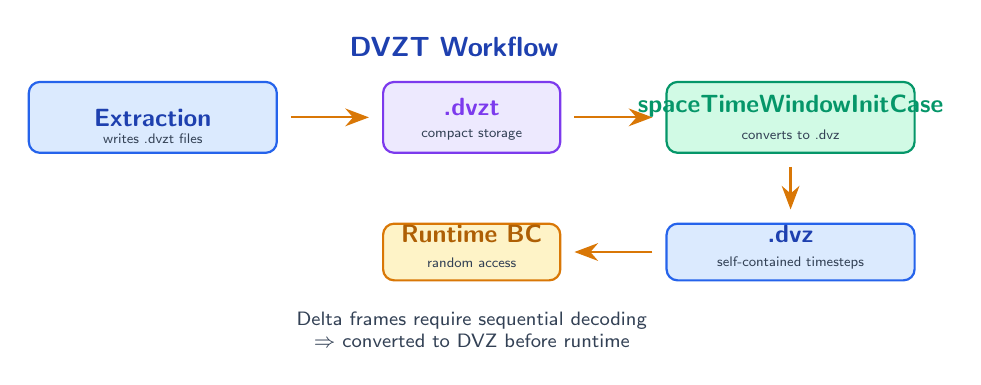
\begin{tikzpicture}[scale=0.9]
    % Title
    \node[font=\sffamily\bfseries, color=primarydark] at (6,5.5) {DVZT Workflow};

    % Extraction phase
    \draw[primaryblue, thick, fill=primarylight, rounded corners=4pt] (0,4) rectangle (3.5,5);
    \node[font=\small\sffamily\bfseries, color=primarydark] at (1.75,4.5) {Extraction};
    \node[font=\tiny\sffamily, color=bodytext] at (1.75,4.2) {writes .dvzt files};

    % Arrow
    \draw[-{Stealth[length=3mm]}, thick, warningorange] (3.7,4.5) -- (4.8,4.5);

    % DVZT files
    \draw[accentpurple, thick, fill=accentlight, rounded corners=4pt] (5,4) rectangle (7.5,5);
    \node[font=\small\sffamily\bfseries, color=accentpurple] at (6.25,4.65) {.dvzt};
    \node[font=\tiny\sffamily, color=bodytext] at (6.25,4.25) {compact storage};

    % Arrow
    \draw[-{Stealth[length=3mm]}, thick, warningorange] (7.7,4.5) -- (8.8,4.5);

    % InitCase
    \draw[secondarygreen, thick, fill=secondarylight, rounded corners=4pt] (9,4) rectangle (12.5,5);
    \node[font=\small\sffamily\bfseries, color=secondarygreen] at (10.75,4.65) {spaceTimeWindowInitCase};
    \node[font=\tiny\sffamily, color=bodytext] at (10.75,4.25) {converts to .dvz};

    % Arrow down
    \draw[-{Stealth[length=3mm]}, thick, warningorange] (10.75,3.8) -- (10.75,3.2);

    % DVZ files
    \draw[primaryblue, thick, fill=primarylight, rounded corners=4pt] (9,2.2) rectangle (12.5,3);
    \node[font=\small\sffamily\bfseries, color=primarydark] at (10.75,2.85) {.dvz};
    \node[font=\tiny\sffamily, color=bodytext] at (10.75,2.45) {self-contained timesteps};

    % Arrow
    \draw[-{Stealth[length=3mm]}, thick, warningorange] (8.8,2.6) -- (7.7,2.6);

    % Runtime
    \draw[warningorange, thick, fill=warninglight, rounded corners=4pt] (5,2.2) rectangle (7.5,3);
    \node[font=\small\sffamily\bfseries, color=warningorange!80!black] at (6.25,2.85) {Runtime BC};
    \node[font=\tiny\sffamily, color=bodytext] at (6.25,2.45) {random access};

    % Notes
    \node[font=\scriptsize\sffamily, color=bodytext, align=center] at (6.25,1.5) {Delta frames require sequential decoding\\$\Rightarrow$ converted to DVZ before runtime};
\end{tikzpicture}
\caption{DVZT workflow: extraction writes compact .dvzt files. Before reconstruction, spaceTimeWindowInitCase converts them to .dvz format (required for random timestep access at runtime)}
\label{fig:dvzt-workflow}
\end{figure}

\begin{lstlisting}[language=OpenFOAM,caption={DVZT configuration}]
writeFormat             dvzt;
deltaVarintPrecision    6;        // ~1e-6 relative precision
dvztKeyframeInterval    20;       // Keyframe every 20 timesteps (default)
\end{lstlisting}

\subsubsection{DVZT Mathematical Formulation}

\paragraph{Frame Types}

DVZT distinguishes between keyframes and delta frames based on the timestep index $k$ (\cref{eq:dvzt-frame-type}):
\begin{equation}
    \text{Frame type}(k) = \begin{cases}
        \text{Keyframe} & \text{if } k \mod K = 0 \\
        \text{Delta frame} & \text{otherwise}
    \end{cases}
    \label{eq:dvzt-frame-type}
\end{equation}
where $K$ is the keyframe interval (default $K = 20$).

\paragraph{Keyframe Encoding}

Keyframes use pure DVZ encoding (spatial delta only), as shown in \cref{eq:dvzt-keyframe}:
\begin{equation}
    \delta_i^{(k)} = v_i^{(k)} - v_{i-1}^{(k)} \quad \text{(spatial delta)}
    \label{eq:dvzt-keyframe}
\end{equation}

\paragraph{Delta Frame Hybrid Prediction}

Delta frames use a weighted combination of spatial and temporal neighbors (\cref{eq:dvzt-prediction}):
\begin{equation}
    \hat{v}_i^{(k)} = \alpha \cdot v_{i-1}^{(k)} + (1 - \alpha) \cdot v_i^{(k-1)}
    \label{eq:dvzt-prediction}
\end{equation}
where $\alpha = 0.3$ (30\% spatial weight, 70\% temporal weight).

The residual to be encoded is given by \cref{eq:dvzt-residual}:
\begin{equation}
    r_i^{(k)} = v_i^{(k)} - \hat{v}_i^{(k)}
    \label{eq:dvzt-residual}
\end{equation}

For slowly varying flows with small $\Delta t$, consecutive timesteps are nearly identical, so $v_i^{(k)} \approx v_i^{(k-1)}$, making the temporal prediction highly accurate and $|r_i^{(k)}| \ll |v_i^{(k)} - v_{i-1}^{(k)}|$.

\paragraph{Compression Ratio Analysis}

Let $\sigma_s^2$ be the variance of spatial deltas and $\sigma_t^2$ the variance of temporal deltas. The hybrid prediction residual variance is approximately (\cref{eq:dvzt-variance}):
\begin{equation}
    \sigma_r^2 \approx \alpha^2 \sigma_s^2 + (1-\alpha)^2 \sigma_t^2
    \label{eq:dvzt-variance}
\end{equation}

For small timesteps where $\sigma_t^2 \ll \sigma_s^2$ (\cref{eq:dvzt-ratio}):
\begin{equation}
    \frac{\sigma_r}{\sigma_s} \approx \alpha = 0.3
    \label{eq:dvzt-ratio}
\end{equation}

This explains the $\sim$70\% reduction in residual magnitude, which translates to significant compression improvement through varint encoding.

\paragraph{Decoding Dependency}

Delta frames depend on the previous frame for reconstruction (\cref{eq:dvzt-decode}):
\begin{equation}
    v_i^{(k)} = r_i^{(k)} + \alpha \cdot v_{i-1}^{(k)} + (1 - \alpha) \cdot v_i^{(k-1)}
    \label{eq:dvzt-decode}
\end{equation}

This creates a dependency chain from each keyframe (\cref{eq:dvzt-chain}):
\begin{equation}
    \text{Keyframe } k_0 \rightarrow \text{Frame } k_0+1 \rightarrow \cdots \rightarrow \text{Frame } k_0+K-1
    \label{eq:dvzt-chain}
\end{equation}

Random access requires decoding from the nearest preceding keyframe. For this reason, the initialization utility converts DVZT to DVZ before runtime.

\textbf{DVZT Workflow:}

During extraction, DVZT writes smaller \texttt{.dvzt} files. During case initialization, the utility automatically converts \texttt{.dvzt} to \texttt{.dvz} format (required because delta frames need sequential processing). The resulting \texttt{.dvz} files are read by the spaceTimeWindow BC at runtime.

\begin{center}
Extraction $\rightarrow$ \texttt{.dvzt} files ($\sim$10\% smaller) $\rightarrow$ \texttt{spaceTimeWindowInitCase} $\rightarrow$ \texttt{.dvz} files $\rightarrow$ Runtime
\end{center}

\textbf{When to use DVZT:}
\begin{itemize}
    \item Long simulations with many timesteps (storage savings accumulate)
    \item Network/disk bandwidth constraints during extraction
    \item Small timesteps ($\Delta t = 10^{-5}$ or $10^{-6}$) where temporal correlation is very strong
    \item DNS or acoustic simulations requiring fine temporal resolution
\end{itemize}

\textbf{Compression vs Timestep Size:}

DVZT benefits increase dramatically with smaller timesteps because consecutive values become nearly identical (see \cref{tab:dvzt-compression}):

\begin{table}[htbp]
\centering
\caption{DVZT compression improvement by timestep size}
\label{tab:dvzt-compression}
\begin{tabular}{@{}lll@{}}
\toprule
\textbf{$\Delta t$} & \textbf{Temporal Correlation} & \textbf{DVZT vs DVZ Savings} \\
\midrule
$10^{-4}$ & Moderate & $\sim$10\% smaller \\
$10^{-5}$ & Strong & $\sim$20--30\% smaller \\
$10^{-6}$ & Very strong & $\sim$30--50\% smaller \\
\bottomrule
\end{tabular}
\end{table}

\textbf{When to use DVZ:}
\begin{itemize}
    \item Simpler workflow (no conversion step)
    \item When random access to individual timesteps is needed during extraction
    \item Shorter simulations where DVZT overhead isn't worth it
    \item Large timesteps where temporal correlation is weak
\end{itemize}

\subsubsection{External Compression Benchmark}

DVZ and DVZT files can be further compressed using external tools for archival or transfer. The following benchmarks compare various compression algorithms on real boundary data files.

\textbf{Test Environment:}
\begin{itemize}
    \item \textbf{CPU}: Intel Core i7-4790 @ 3.60~GHz (4 cores, 8 threads, Haswell microarchitecture)
    \item \textbf{L3 Cache}: 8~MB
    \item \textbf{RAM}: DDR3-1600
\end{itemize}

\textbf{Test Data:} 618 DVZ files totaling 13~MB (spatial delta-varint encoded), and 938 DVZT files totaling 30~MB (temporal delta-varint encoded).

The compression results are presented in \cref{tab:ext-compression-dvz} for DVZ files and \cref{tab:ext-compression-dvzt} for DVZT files.

\begin{table}[htbp]
\centering
\caption{External compression results for DVZ files (13~MB original)}
\label{tab:ext-compression-dvz}
\small
\begin{tabular}{@{}llrrl@{}}
\toprule
\textbf{Method} & \textbf{Size} & \textbf{Ratio} & \textbf{Speed} & \textbf{Notes} \\
\midrule
7z lzma2 -mx9 & 769~KB & 6.01\% & 11.2~MB/s & Best ratio \\
xz -6 & 769~KB & 6.01\% & 10.2~MB/s & \\
zstd --ultra -22 & 964~KB & 7.53\% & 4.7~MB/s & Very slow \\
zstd -19 & 965~KB & 7.54\% & 15.3~MB/s & \\
rar -m5 & 1017~KB & 7.95\% & 26.9~MB/s & \\
7z ppmd -mx9 & 1.4~MB & 11.02\% & 10.7~MB/s & \\
zstd -9 & 1.7~MB & 13.17\% & 109.5~MB/s & \\
zstd -3 & 1.8~MB & 13.65\% & 309.0~MB/s & Best balance \\
zstd -1 & 1.9~MB & 14.43\% & 533.7~MB/s & \\
bzip2 -9 & 2.0~MB & 15.28\% & 13.5~MB/s & \\
gzip -6 & 2.1~MB & 16.39\% & 94.2~MB/s & \\
lz4 & 2.3~MB & 17.80\% & 635.2~MB/s & Fastest \\
\bottomrule
\end{tabular}
\end{table}

\begin{table}[htbp]
\centering
\caption{External compression results for DVZT files (30~MB original)}
\label{tab:ext-compression-dvzt}
\small
\begin{tabular}{@{}llrrl@{}}
\toprule
\textbf{Method} & \textbf{Size} & \textbf{Ratio} & \textbf{Speed} & \textbf{Notes} \\
\midrule
7z lzma2 -mx9 & 1.9~MB & 6.31\% & 10.1~MB/s & Best ratio \\
xz -6 & 1.9~MB & 6.32\% & 10.5~MB/s & \\
zstd --ultra -22 & 2.6~MB & 8.48\% & 2.4~MB/s & Very slow \\
zstd -19 & 2.6~MB & 8.50\% & 10.4~MB/s & \\
rar -m5 & 2.8~MB & 9.28\% & 28.0~MB/s & \\
zstd -9 & 2.8~MB & 9.27\% & 120.6~MB/s & \\
7z ppmd -mx9 & 2.8~MB & 9.37\% & 12.2~MB/s & \\
zstd -3 & 3.1~MB & 10.10\% & 396.1~MB/s & Best balance \\
zstd -1 & 3.1~MB & 10.25\% & 614.0~MB/s & \\
bzip2 -9 & 3.5~MB & 11.52\% & 13.7~MB/s & \\
gzip -6 & 3.8~MB & 12.71\% & 104.3~MB/s & \\
lz4 & 4.1~MB & 13.56\% & 763.0~MB/s & Fastest \\
\bottomrule
\end{tabular}
\end{table}

\textbf{Key findings:}
\begin{itemize}
    \item \textbf{Best compression ratio}: 7z LZMA2 and xz achieve $\sim$6\% (94\% reduction)
    \item \textbf{Best speed/ratio balance}: zstd -3 at 10--14\% ratio with 300--400~MB/s throughput
    \item \textbf{zstd -3 is 40$\times$ faster than xz} with only 60\% more space
    \item \textbf{zstd --ultra -22 provides no benefit} over zstd -19 for this data type
    \item \textbf{bzip2 and PPMd perform poorly} for CFD boundary data
\end{itemize}

\textbf{Recommendations:}
\begin{itemize}
    \item \textbf{Runtime/on-the-fly}: zstd -3 ($\sim$10\% ratio, 300--400~MB/s)
    \item \textbf{Archive/transfer}: 7z lzma2 -mx9 or xz -6 ($\sim$6\% ratio, 10~MB/s)
    \item \textbf{Real-time streaming}: lz4 ($\sim$14--18\% ratio, 600--800~MB/s)
\end{itemize}

\begin{lstlisting}[language=bash,caption={Archival compression example}]
# Archive with best compression (7z)
cd subset-case/constant/boundaryData/oldInternalFaces
7z a -m0=lzma2 -mx=9 ../boundaryData.7z */U.dvz */U.dvzt

# Or with zstd for faster compression
tar -cf - */U.dvz */U.dvzt | zstd -3 > ../boundaryData.tar.zst
\end{lstlisting}

\subsection{Extraction Metadata}

The \texttt{extractionMetadata} file contains:

\begin{lstlisting}[language=OpenFOAM,caption={extractionMetadata contents}]
{
    openfoamVersion     "v2512";
    openfoamApi         2512;
    solver              "pimpleFoam";
    deltaT              1e-04;
    adjustTimeStep      false;
    timePrecision       6;
    extractionStartTime 0.0001;
    boxMin              (0.05 -0.25 0.01);
    boxMax              (0.90 0.25 0.38);
    nGlobalFaces        12345;
    timesteps           (0.0001 0.0002 0.0003 ...);
}
\end{lstlisting}

% ----------------------------------------------------------------------------
% PARALLEL EXECUTION
% ----------------------------------------------------------------------------

\section{Parallel Execution}
\label{sec:parallel}

Both the source simulation (extraction phase) and the reconstruction simulation can run in parallel. This enables efficient use of HPC resources for both phases of the workflow.

\subsection{Parallel Extraction}

The extraction function object fully supports parallel execution:

\begin{itemize}
    \item Extraction box can span multiple processor domains
    \item Boundary data is gathered from all processors
    \item Master processor writes combined data files
    \item Processor boundary faces are handled automatically
\end{itemize}

\begin{lstlisting}[language=bash,caption={Parallel extraction}]
# Decompose the case
decomposePar

# Run parallel extraction
mpirun -np 8 pimpleFoam -parallel

# Automatic field writes occur at:
#   t_0 - extraction start (for lookback)
#   t_1 - linear interpolation start
#   t_2 - cubic interpolation start
\end{lstlisting}

\subsection{Field Reconstruction}

After parallel extraction, reconstruct fields before case initialization:

\begin{lstlisting}[language=bash,caption={Field reconstruction}]
# For cubic interpolation (recommended)
reconstructPar -time <t_2>

# For linear interpolation
reconstructPar -time <t_1>
\end{lstlisting}

\begin{warningbox}
The subset mesh created by \texttt{spaceTimeWindowInitCase} uses cell ordering from the reconstructed (serial) source mesh. Running \texttt{reconstructPar} before case initialization is mandatory for parallel extractions.
\end{warningbox}

\subsection{Parallel Reconstruction}

The reconstruction simulation can also run in parallel, independently of how the extraction was performed:

\begin{lstlisting}[language=bash,caption={Parallel reconstruction}]
cd subset-case
decomposePar
mpirun -np 4 pimpleFoam -parallel
reconstructPar
\end{lstlisting}

\begin{tipbox}
The reconstruction case is typically much smaller than the source case, so fewer processors may be needed. The spaceTimeWindow boundary conditions work identically in serial and parallel modes.
\end{tipbox}

% ----------------------------------------------------------------------------
% MASS CONSERVATION
% ----------------------------------------------------------------------------

\section{Mass Conservation}
\label{sec:mass}

\subsection{The Mass Imbalance Problem}

Face interpolation during extraction can introduce small mass flux imbalances:
\begin{equation}
    \text{imbalance} = \sum_f \mathbf{U}_f \cdot \mathbf{S}_f \neq 0
\end{equation}

When all boundary patches have \texttt{fixesValue=true}, \texttt{adjustPhi()} cannot correct this imbalance, potentially causing pressure solver issues. Additionally, with all-Dirichlet BCs, the solver has no way to relieve pressure buildup.

\subsection{Solutions}

\subsubsection{Use \texttt{-inletOutletBC} (Recommended)}

The flux-based inlet-outlet BC naturally handles mass conservation:
\begin{itemize}
    \item Outflow faces use zeroGradient, allowing natural outflow
    \item No artificial mass imbalance from prescribed outflow velocities
    \item Works without any special mass correction
\end{itemize}

\begin{lstlisting}[language=bash,caption={Using inlet-outlet BC for mass conservation}]
spaceTimeWindowInitCase -sourceCase ../source -inletOutletBC
\end{lstlisting}

\subsubsection{Use \texttt{-correctMassFlux}}

Applies least-squares correction to boundaryData to ensure exact mass conservation:

\begin{equation}
    \mathbf{U}_{\text{corrected}} = \mathbf{U} - \frac{\text{imbalance}}{\sum_f |\mathbf{S}_f|} \cdot \hat{\mathbf{n}}
\end{equation}

where $\hat{\mathbf{n}} = \mathbf{S}_f / |\mathbf{S}_f|$ is the face unit normal.

This minimizes $\|\mathbf{U}_{\text{corrected}} - \mathbf{U}\|^2$ subject to:
\begin{equation}
    \sum_f \mathbf{U}_{\text{corrected}} \cdot \mathbf{S}_f = 0
\end{equation}

\begin{lstlisting}[language=bash,caption={Using mass flux correction}]
spaceTimeWindowInitCase -sourceCase ../source -inletOutletBC -correctMassFlux
\end{lstlisting}

\subsubsection{Use \texttt{-outletDirection} with \texttt{fixesValue true}}

Creates an outlet patch where mass imbalance can escape:
\begin{itemize}
    \item \texttt{oldInternalFaces} uses \texttt{fixesValue true} (values not modified by adjustPhi)
    \item \texttt{outlet} uses \texttt{inletOutlet} BC (allows adjustPhi correction)
\end{itemize}

\subsection{The \texttt{fixesValue} Option}

The \texttt{fixesValue} parameter controls \texttt{adjustPhi()} behavior:

\begin{itemize}
    \item \texttt{fixesValue = true}: Patch excluded from flux correction (preserves exact values)
    \item \texttt{fixesValue = false}: Patch included in flux correction (allows modification)
\end{itemize}

\subsection{Outlet Patch for Pressure Relief}

The \texttt{-outletDirection} option creates an outlet patch (see \cref{fig:outlet-patch}):

\begin{lstlisting}[language=bash,caption={Creating outlet patch}]
spaceTimeWindowInitCase -sourceCase ../source \
    -outletDirection "(1 0 0)" \
    -outletFraction 0.1
\end{lstlisting}

\begin{figure}[htbp]
\centering
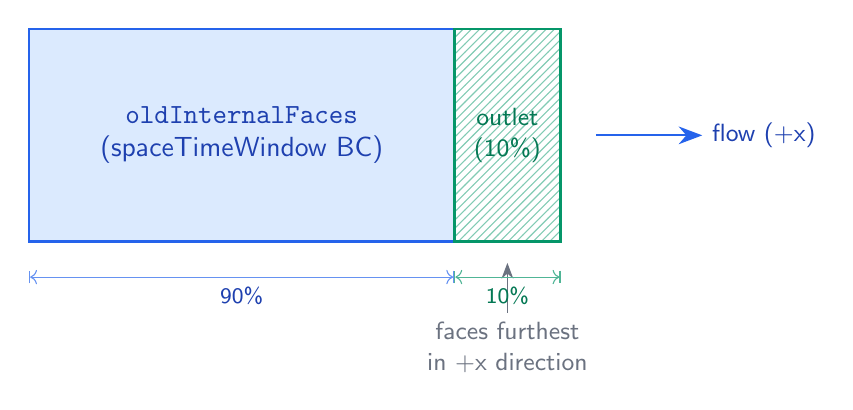
\begin{tikzpicture}[scale=0.9]
    % Main box (oldInternalFaces region)
    \draw[thick, fill=primarylight, draw=primaryblue, line width=1pt] (0,0) rectangle (6,3);

    % Outlet region (hatched)
    \draw[thick, fill=secondarylight, draw=secondarygreen, line width=1pt, pattern=north east lines, pattern color=secondarygreen!50] (6,0) rectangle (7.5,3);

    % Labels inside boxes
    \node[align=center, color=primarydark, font=\sffamily] at (3,1.5) {\texttt{oldInternalFaces}\\(spaceTimeWindow BC)};
    \node[align=center, font=\small\sffamily, color=secondarygreen!80!black] at (6.75,1.5) {outlet\\(10\%)};

    % Flow direction arrow
    \draw[-{Stealth[length=3mm]}, thick, color=primaryblue] (8,1.5) -- (9.5,1.5);
    \node[right, font=\small\sffamily, color=primarydark] at (9.5,1.5) {flow (+x)};

    % Annotation for outlet selection
    \draw[{Stealth[length=2mm]}-, color=codecomment] (6.75,-0.3) -- (6.75,-1);
    \node[below, font=\small\sffamily, align=center, color=codecomment] at (6.75,-1) {faces furthest\\in +x direction};

    % Dimension indication
    \draw[|<->|, color=primaryblue!70] (0,-0.5) -- (6,-0.5);
    \node[below, font=\footnotesize\sffamily, color=primarydark] at (3,-0.5) {90\%};
    \draw[|<->|, color=secondarygreen!70] (6,-0.5) -- (7.5,-0.5);
    \node[below, font=\footnotesize\sffamily, color=secondarygreen!80!black] at (6.75,-0.5) {10\%};
\end{tikzpicture}
\caption{Outlet patch creation with \texttt{-outletDirection "(1 0 0)"}}
\label{fig:outlet-patch}
\end{figure}

Outlet faces are selected based on position (furthest along the outlet direction), not face orientation.

\subsection{Recommended Configurations}

The recommended mass conservation strategies are summarized in \cref{tab:mass-strategies}.

\begin{table}[htbp]
\centering
\caption{Mass conservation strategies}
\label{tab:mass-strategies}
\begin{tabularx}{\textwidth}{@{}lX@{}}
\toprule
\textbf{Configuration} & \textbf{Description} \\
\midrule
\texttt{-inletOutletBC} &
\textbf{Recommended} for unsteady turbulent flows (vortex shedding, etc.). Natural mass balance through flux-based switching. \\
\addlinespace
\texttt{-inletOutletBC -correctMassFlux} &
Unsteady turbulent + extra safety. Ensures exact mass balance with inlet-outlet switching. \\
\addlinespace
\texttt{-outletDirection "(1 0 0)"} &
Steady-mean flow direction. Use when outlet location is known and flow direction is consistent. \\
\addlinespace
\texttt{-correctMassFlux} (no outlet) &
Maximum fidelity. All faces prescribed with exact mass balance. \\
\bottomrule
\end{tabularx}
\end{table}

% ----------------------------------------------------------------------------
% SOLVER SETTINGS
% ----------------------------------------------------------------------------

\section{Solver Settings and Relaxation}
\label{sec:solver}

\subsection{Time Stepping}

For accurate reconstruction, use identical time stepping:

\begin{lstlisting}[language=OpenFOAM,caption={Recommended controlDict settings}]
deltaT          1e-04;      // Must match extraction
adjustTimeStep  no;         // Fixed timestep recommended

// If adaptive timestep is required:
adjustTimeStep  yes;
maxCo           0.5;
maxDeltaT       1e-03;
\end{lstlisting}

\begin{warningbox}
The reconstruction must use identical \texttt{deltaT} and \texttt{adjustTimeStep} settings as the extraction. Mismatches cause fatal errors unless \texttt{allowTimeInterpolation=true}.
\end{warningbox}

\subsection{PIMPLE Settings}

For incompressible flows:

\begin{lstlisting}[language=OpenFOAM,caption={Recommended PIMPLE settings}]
PIMPLE
{
    nOuterCorrectors    2;
    nCorrectors         2;
    nNonOrthogonalCorrectors 1;

    // Pressure reference (set by spaceTimeWindowInitCase)
    pRefPoint           (0.5 0 0.2);
    pRefValue           0;
}
\end{lstlisting}

\subsection{Relaxation Factors}

\begin{tipbox}
For reconstruction simulations, relaxation is typically \textbf{not needed} because:
\begin{itemize}
    \item Boundary conditions are prescribed (not coupled)
    \item Initial conditions come from the source simulation
    \item Flow field evolves smoothly from physical initial state
\end{itemize}
\end{tipbox}

If stability issues occur, try:

\begin{lstlisting}[language=OpenFOAM,caption={Optional relaxation}]
relaxationFactors
{
    fields
    {
        p               0.7;
    }
    equations
    {
        U               0.7;
        "(k|epsilon|omega|nuTilda)"  0.7;
    }
}
\end{lstlisting}

\subsection{Linear Solver Settings}

Standard settings work well:

\begin{lstlisting}[language=OpenFOAM,caption={Linear solver settings}]
solvers
{
    p
    {
        solver          GAMG;
        smoother        GaussSeidel;
        tolerance       1e-06;
        relTol          0.01;
    }

    U
    {
        solver          PBiCGStab;
        preconditioner  DILU;
        tolerance       1e-06;
        relTol          0.1;
    }
}
\end{lstlisting}

% ----------------------------------------------------------------------------
% TIME INTERPOLATION
% ----------------------------------------------------------------------------

\section{Time Interpolation}
\label{sec:interpolation}

The boundary conditions support three time interpolation modes, summarized in \Cref{tab:time-interp-modes} and illustrated in \cref{fig:time-interp-modes}. The comparison between linear and cubic interpolation quality is shown in \cref{fig:linear-vs-cubic}.

\begin{table}[htbp]
\centering
\caption{Time interpolation modes}
\label{tab:time-interp-modes}
\begin{tabular}{@{}llll@{}}
\toprule
\textbf{Mode} & \textbf{Start Time} & \textbf{Timesteps Used} & \textbf{Use Case} \\
\midrule
\texttt{none} (exact) & $t_0$ & 1 (exact match) & ``Bit''-reproducible results \\
\texttt{linear} & $t_1$ & 2 (bracketing) & Simple, smoothly varying flows \\
\texttt{cubic} & $t_2$ & 4 (Catmull-Rom) & Unsteady turbulent flows (recommended) \\
\bottomrule
\end{tabular}
\end{table}

\texttt{spaceTimeWindowInitCase} automatically sets \texttt{startTime} and \texttt{endTime} to ensure sufficient buffer timesteps for the selected interpolation scheme (see \cref{fig:time-buffer} for buffer requirements).

\begin{figure}[htbp]
\centering
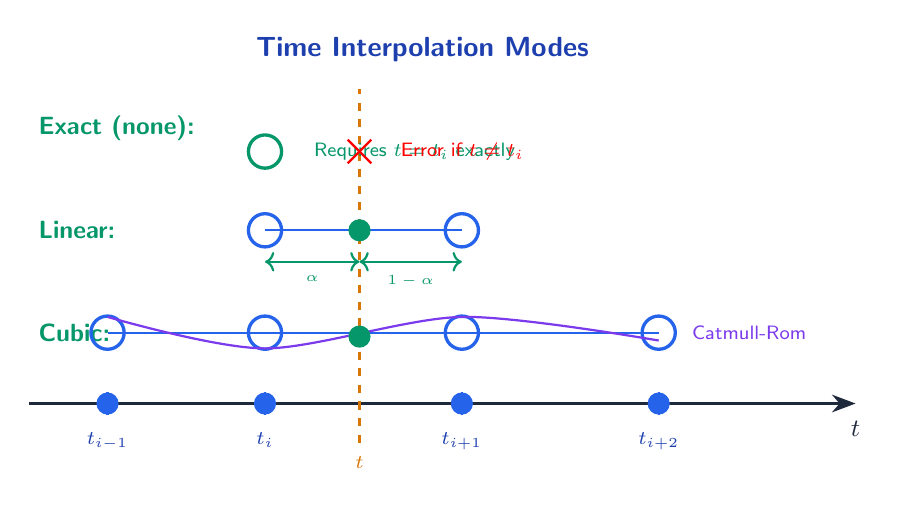
\begin{tikzpicture}[scale=1.0]
    % Title
    \node[font=\sffamily\bfseries, color=primarydark] at (5,4.5) {Time Interpolation Modes};

    % Time axis
    \draw[-{Stealth[length=3mm]}, thick, headingcolor] (0,0) -- (10.5,0);
    \node[below, font=\small\sffamily, color=headingcolor] at (10.5,-0.1) {$t$};

    % Timestep markers (available data points)
    \foreach \x/\label in {1/$t_{i-1}$, 3/$t_i$, 5.5/$t_{i+1}$, 8/$t_{i+2}$} {
        \draw[primaryblue, thick] (\x,-0.15) -- (\x,0.15);
        \node[below, font=\scriptsize\sffamily, color=primarydark] at (\x,-0.25) {\label};
        \fill[primaryblue] (\x,0) circle (4pt);
    }

    % Query time marker
    \draw[warningorange, thick, dashed] (4.2,-0.5) -- (4.2,4);
    \node[below, font=\scriptsize\sffamily\bfseries, color=warningorange] at (4.2,-0.55) {$t$};

    % === EXACT (none) ===
    \node[font=\small\sffamily\bfseries, color=secondarygreen, anchor=west] at (0,3.5) {Exact (none):};
    % Show exact match required
    \draw[secondarygreen, very thick] (3,3.2) circle (6pt);
    \node[font=\scriptsize\sffamily, color=secondarygreen, anchor=west] at (3.5,3.2) {Requires $t = t_i$ exactly};
    % X mark at query time
    \draw[red, thick] (4.05,3.05) -- (4.35,3.35);
    \draw[red, thick] (4.05,3.35) -- (4.35,3.05);
    \node[font=\scriptsize\sffamily, color=red, anchor=west] at (4.6,3.2) {Error if $t \neq t_i$};

    % === LINEAR ===
    \node[font=\small\sffamily\bfseries, color=secondarygreen, anchor=west] at (0,2.2) {Linear:};
    % Show two bracketing points
    \draw[primaryblue, very thick] (3,2.2) circle (6pt);
    \draw[primaryblue, very thick] (5.5,2.2) circle (6pt);
    \draw[primaryblue, thick] (3,2.2) -- (5.5,2.2);
    % Interpolated point
    \fill[secondarygreen] (4.2,2.2) circle (4pt);
    % Alpha label
    \draw[<->, secondarygreen, thick] (3,1.8) -- (4.2,1.8);
    \node[below, font=\tiny\sffamily, color=secondarygreen] at (3.6,1.75) {$\alpha$};
    \draw[<->, secondarygreen, thick] (4.2,1.8) -- (5.5,1.8);
    \node[below, font=\tiny\sffamily, color=secondarygreen] at (4.85,1.75) {$1-\alpha$};

    % === CUBIC ===
    \node[font=\small\sffamily\bfseries, color=secondarygreen, anchor=west] at (0,0.9) {Cubic:};
    % Show four points
    \draw[primaryblue, very thick] (1,0.9) circle (6pt);
    \draw[primaryblue, very thick] (3,0.9) circle (6pt);
    \draw[primaryblue, very thick] (5.5,0.9) circle (6pt);
    \draw[primaryblue, very thick] (8,0.9) circle (6pt);
    % Draw smooth curve through points
    \draw[primaryblue, thick, smooth] plot coordinates {(1,0.9) (3,0.9) (5.5,0.9) (8,0.9)};
    % Catmull-Rom spline visual (curved)
    \draw[accentpurple, thick, smooth, tension=0.5] plot coordinates {(1,1.1) (3,0.7) (5.5,1.1) (8,0.8)};
    % Interpolated point on curve
    \fill[secondarygreen] (4.2,0.85) circle (4pt);
    \node[font=\scriptsize\sffamily, color=accentpurple, anchor=west] at (8.3,0.9) {Catmull-Rom};
\end{tikzpicture}
\caption{Time interpolation modes: exact matching uses only one timestep, linear interpolation uses two bracketing timesteps, and cubic (Catmull-Rom) uses four timesteps for smooth $C^1$ continuous interpolation}
\label{fig:time-interp-modes}
\end{figure}

\begin{figure}[htbp]
\centering
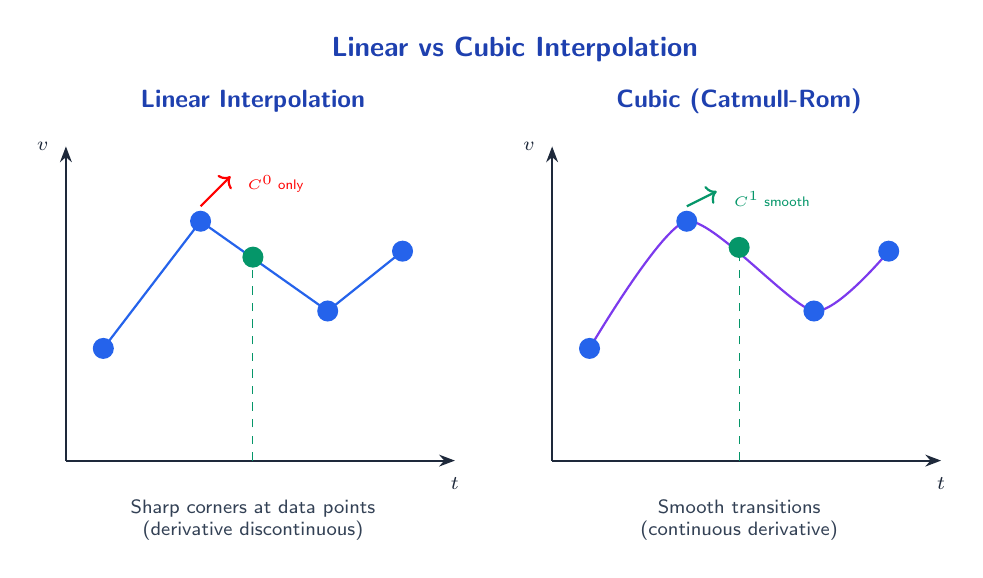
\begin{tikzpicture}[scale=0.95]
    % Title
    \node[font=\sffamily\bfseries, color=primarydark] at (6,5.5) {Linear vs Cubic Interpolation};

    % === Left side: Linear ===
    \node[font=\small\sffamily\bfseries, color=primarydark] at (2.5,4.8) {Linear Interpolation};

    % Axes
    \draw[-{Stealth[length=2mm]}, thick, headingcolor] (0,0) -- (5.2,0);
    \draw[-{Stealth[length=2mm]}, thick, headingcolor] (0,0) -- (0,4.2);
    \node[below, font=\scriptsize\sffamily, color=headingcolor] at (5.2,-0.1) {$t$};
    \node[left, font=\scriptsize\sffamily, color=headingcolor] at (-0.1,4.2) {$v$};

    % Data points with values (non-uniform spacing)
    \coordinate (P0) at (0.5,1.5);
    \coordinate (P1) at (1.8,3.2);
    \coordinate (P2) at (3.5,2.0);
    \coordinate (P3) at (4.5,2.8);

    % Draw linear segments
    \draw[primaryblue, thick] (P0) -- (P1) -- (P2) -- (P3);

    % Data points
    \fill[primaryblue] (P0) circle (4pt);
    \fill[primaryblue] (P1) circle (4pt);
    \fill[primaryblue] (P2) circle (4pt);
    \fill[primaryblue] (P3) circle (4pt);

    % Query point
    \fill[secondarygreen] (2.5,2.72) circle (4pt);
    \draw[secondarygreen, dashed] (2.5,0) -- (2.5,2.72);

    % Highlight discontinuity in derivative
    \draw[red, thick, ->] (1.8,3.4) -- (2.2,3.8);
    \node[font=\tiny\sffamily, color=red, anchor=west] at (2.3,3.7) {$C^0$ only};

    % === Right side: Cubic ===
    \node[font=\small\sffamily\bfseries, color=primarydark] at (9,4.8) {Cubic (Catmull-Rom)};

    % Axes
    \draw[-{Stealth[length=2mm]}, thick, headingcolor] (6.5,0) -- (11.7,0);
    \draw[-{Stealth[length=2mm]}, thick, headingcolor] (6.5,0) -- (6.5,4.2);
    \node[below, font=\scriptsize\sffamily, color=headingcolor] at (11.7,-0.1) {$t$};
    \node[left, font=\scriptsize\sffamily, color=headingcolor] at (6.4,4.2) {$v$};

    % Data points (same positions, shifted right)
    \coordinate (Q0) at (7,1.5);
    \coordinate (Q1) at (8.3,3.2);
    \coordinate (Q2) at (10,2.0);
    \coordinate (Q3) at (11,2.8);

    % Draw smooth Catmull-Rom spline
    \draw[accentpurple, thick, smooth, tension=0.4] plot coordinates {(Q0) (Q1) (Q2) (Q3)};

    % Data points
    \fill[primaryblue] (Q0) circle (4pt);
    \fill[primaryblue] (Q1) circle (4pt);
    \fill[primaryblue] (Q2) circle (4pt);
    \fill[primaryblue] (Q3) circle (4pt);

    % Query point (on smooth curve)
    \fill[secondarygreen] (9,2.85) circle (4pt);
    \draw[secondarygreen, dashed] (9,0) -- (9,2.85);

    % Highlight smooth derivative
    \draw[secondarygreen, thick, ->] (8.3,3.4) -- (8.7,3.6);
    \node[font=\tiny\sffamily, color=secondarygreen, anchor=west] at (8.8,3.5) {$C^1$ smooth};

    % Labels below
    \node[font=\scriptsize\sffamily, color=bodytext, align=center] at (2.5,-0.8) {Sharp corners at data points\\(derivative discontinuous)};
    \node[font=\scriptsize\sffamily, color=bodytext, align=center] at (9,-0.8) {Smooth transitions\\(continuous derivative)};
\end{tikzpicture}
\caption{Comparison of linear and cubic interpolation: linear interpolation creates $C^0$ continuous curves with sharp corners at data points, while Catmull-Rom cubic splines provide $C^1$ continuity with smooth transitions}
\label{fig:linear-vs-cubic}
\end{figure}

\begin{figure}[htbp]
\centering
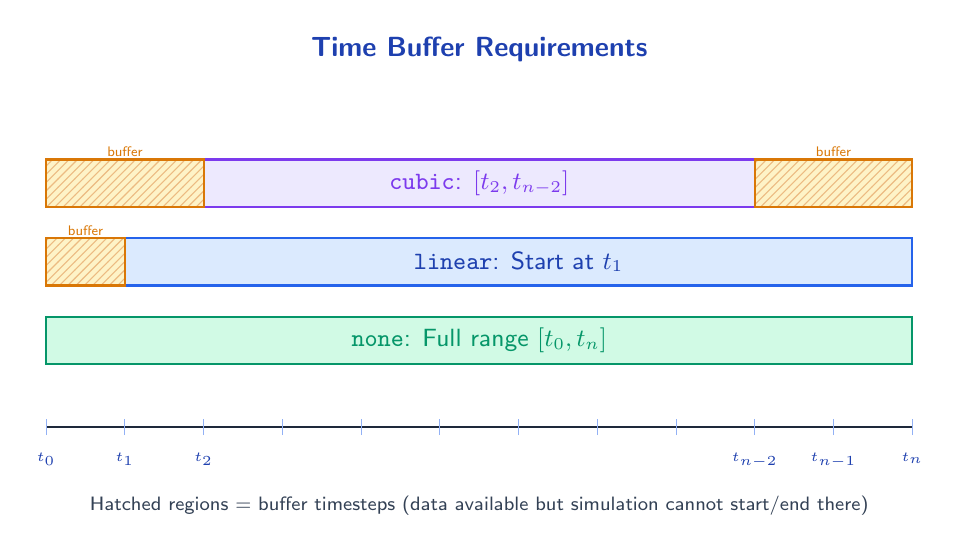
\begin{tikzpicture}[scale=1.0]
    % Title
    \node[font=\sffamily\bfseries, color=primarydark] at (5.5,4.8) {Time Buffer Requirements};

    % Timeline
    \draw[thick, headingcolor] (0,0) -- (11,0);

    % All timesteps
    \foreach \x in {0,1,2,3,4,5,6,7,8,9,10,11} {
        \draw[primaryblue!50] (\x,-0.1) -- (\x,0.1);
    }

    % Labels for key timesteps
    \node[below, font=\tiny\sffamily, color=primarydark] at (0,-0.2) {$t_0$};
    \node[below, font=\tiny\sffamily, color=primarydark] at (1,-0.2) {$t_1$};
    \node[below, font=\tiny\sffamily, color=primarydark] at (2,-0.2) {$t_2$};
    \node[below, font=\tiny\sffamily, color=primarydark] at (9,-0.2) {$t_{n-2}$};
    \node[below, font=\tiny\sffamily, color=primarydark] at (10,-0.2) {$t_{n-1}$};
    \node[below, font=\tiny\sffamily, color=primarydark] at (11,-0.2) {$t_n$};

    % === Exact mode ===
    \fill[secondarylight] (0,0.8) rectangle (11,1.4);
    \draw[secondarygreen, thick] (0,0.8) rectangle (11,1.4);
    \node[font=\small\sffamily, color=secondarygreen] at (5.5,1.1) {\texttt{none}: Full range $[t_0, t_n]$};

    % === Linear mode ===
    \fill[primarylight] (1,1.8) rectangle (11,2.4);
    \draw[primaryblue, thick] (1,1.8) rectangle (11,2.4);
    \fill[warninglight] (0,1.8) rectangle (1,2.4);
    \draw[warningorange, thick, pattern=north east lines, pattern color=warningorange!50] (0,1.8) rectangle (1,2.4);
    \node[font=\small\sffamily, color=primarydark] at (6,2.1) {\texttt{linear}: Start at $t_1$};
    \node[font=\tiny\sffamily, color=warningorange] at (0.5,2.5) {buffer};

    % === Cubic mode ===
    \fill[accentlight] (2,2.8) rectangle (9,3.4);
    \draw[accentpurple, thick] (2,2.8) rectangle (9,3.4);
    \fill[warninglight] (0,2.8) rectangle (2,3.4);
    \draw[warningorange, thick, pattern=north east lines, pattern color=warningorange!50] (0,2.8) rectangle (2,3.4);
    \fill[warninglight] (9,2.8) rectangle (11,3.4);
    \draw[warningorange, thick, pattern=north east lines, pattern color=warningorange!50] (9,2.8) rectangle (11,3.4);
    \node[font=\small\sffamily, color=accentpurple] at (5.5,3.1) {\texttt{cubic}: $[t_2, t_{n-2}]$};
    \node[font=\tiny\sffamily, color=warningorange] at (1,3.5) {buffer};
    \node[font=\tiny\sffamily, color=warningorange] at (10,3.5) {buffer};

    % Legend
    \node[font=\scriptsize\sffamily, color=bodytext, align=left] at (5.5,-1.0) {Hatched regions = buffer timesteps (data available but simulation cannot start/end there)};
\end{tikzpicture}
\caption{Time buffer requirements for each interpolation mode: exact matching can use the full range, linear needs one buffer timestep at the start, and cubic needs two buffer timesteps at both start and end}
\label{fig:time-buffer}
\end{figure}

\subsection{Exact Timestep Matching (Default)}

By default, the boundary condition requires exact timestep matching:

\begin{itemize}
    \item Simulation time must match available sample times (within 1\% of \texttt{deltaT})
    \item Fatal error if no matching timestep found
    \item Ensures ``bit''-reproducible results (highest fidelity)
\end{itemize}

\subsection{Linear Interpolation}

For cases where exact matching is not possible:

\begin{lstlisting}[language=OpenFOAM,caption={Linear interpolation}]
oldInternalFaces
{
    type                    spaceTimeWindow;
    allowTimeInterpolation  true;
    timeInterpolationScheme linear;
    // ...
}
\end{lstlisting}

Uses two bracketing timesteps (\cref{eq:linear-interp}):
\begin{equation}
    \text{value} = (1 - \alpha) \cdot v_i + \alpha \cdot v_{i+1}
    \quad\text{where}\quad
    \alpha = \frac{t - t_i}{t_{i+1} - t_i}
    \label{eq:linear-interp}
\end{equation}

The interpolation parameter $\alpha \in [0, 1]$ represents the normalized position between the two samples. This is equivalent to first-order polynomial interpolation (\cref{eq:linear-poly}):
\begin{equation}
    \phi(t) = \phi_i + \frac{\phi_{i+1} - \phi_i}{t_{i+1} - t_i}(t - t_i)
    \label{eq:linear-poly}
\end{equation}

Linear interpolation provides $C^0$ continuity (continuous values but discontinuous derivatives at sample points).

\subsection{Cubic Spline Interpolation}

For smoother results with adaptive timestepping:

\begin{lstlisting}[language=OpenFOAM,caption={Cubic interpolation}]
oldInternalFaces
{
    type                    spaceTimeWindow;
    allowTimeInterpolation  true;
    timeInterpolationScheme cubic;
    // ...
}
\end{lstlisting}

Uses centripetal Catmull-Rom spline with four timesteps ($t_{i-1}, t_i, t_{i+1}, t_{i+2}$):

\begin{itemize}
    \item Handles non-uniform time spacing correctly
    \item Provides $C^1$ continuity
    \item No overshoots or cusps
    \item Essential for \texttt{adjustTimeStep=yes}
\end{itemize}

\subsubsection{Catmull-Rom Spline Formulation}

The centripetal Catmull-Rom spline passes through all control points and provides $C^1$ continuity. Given four consecutive sample values $\phi_0, \phi_1, \phi_2, \phi_3$ at times $t_0, t_1, t_2, t_3$, the interpolated value for $t \in [t_1, t_2]$ is computed as follows.

First, compute the centripetal parameterization distances (\cref{eq:catmull-dist}):
\begin{equation}
    d_j = |t_{j+1} - t_j|^{0.5}, \quad j = 0, 1, 2
    \label{eq:catmull-dist}
\end{equation}

The normalized parameter within the segment $[t_1, t_2]$ is (\cref{eq:catmull-param}):
\begin{equation}
    u = \frac{t - t_1}{t_2 - t_1}
    \label{eq:catmull-param}
\end{equation}

The spline is constructed using the Barry-Goldman algorithm. Define intermediate points (\cref{eq:catmull-A}):
\begin{align}
    A_1 &= \frac{t_2 - t}{t_2 - t_0} \phi_0 + \frac{t - t_0}{t_2 - t_0} \phi_1 \nonumber\\
    A_2 &= \frac{t_2 - t}{t_2 - t_1} \phi_1 + \frac{t - t_1}{t_2 - t_1} \phi_2 \label{eq:catmull-A}\\
    A_3 &= \frac{t_3 - t}{t_3 - t_1} \phi_2 + \frac{t - t_1}{t_3 - t_1} \phi_3 \nonumber
\end{align}

Then compute (\cref{eq:catmull-B}):
\begin{align}
    B_1 &= \frac{t_2 - t}{t_2 - t_0} A_1 + \frac{t - t_0}{t_2 - t_0} A_2 \label{eq:catmull-B}\\
    B_2 &= \frac{t_3 - t}{t_3 - t_1} A_2 + \frac{t - t_1}{t_3 - t_1} A_3 \nonumber
\end{align}

Finally, the interpolated value is (\cref{eq:catmull-result}):
\begin{equation}
    \phi(t) = \frac{t_2 - t}{t_2 - t_1} B_1 + \frac{t - t_1}{t_2 - t_1} B_2
    \label{eq:catmull-result}
\end{equation}

This formulation correctly handles non-uniform time spacing, which is essential when adaptive timestepping (\texttt{adjustTimeStep=yes}) produces variable timesteps.

\subsection{Time Range Requirements}

\begin{itemize}
    \item \textbf{Linear}: Needs 2 buffer timesteps at start
    \item \textbf{Cubic}: Needs 2 buffer timesteps at start and end
    \item \texttt{spaceTimeWindowInitCase} automatically sets appropriate \texttt{startTime} and \texttt{endTime}
\end{itemize}

\begin{notebox}
Extrapolation outside the extraction window is \textbf{never} allowed, regardless of interpolation settings.
\end{notebox}

% ----------------------------------------------------------------------------
% FLUX REPORTING
% ----------------------------------------------------------------------------

\section{Flux Reporting and Diagnostics}
\label{sec:diagnostics}

Enable flux reporting to monitor mass conservation:

\begin{lstlisting}[language=OpenFOAM,caption={Enabling flux reporting}]
oldInternalFaces
{
    type            spaceTimeWindow;
    reportFlux      true;
    // ...
}
\end{lstlisting}

Output format (fields explained in \cref{tab:flux-fields}):

\begin{lstlisting}[caption={Flux report output},basicstyle=\tiny\ttfamily]
spaceTimeWindow flux [oldInternalFaces] t=0.001 thisPatch=1.234e-06 (in=-0.0523 out=0.0523) | MESH TOTAL=5.678e-05 (fixed=-0.0523 adjustable=0.0523) | adjustPhi will correct: -5.678e-05
\end{lstlisting}

\begin{table}[htbp]
\centering
\caption{Flux report fields}
\label{tab:flux-fields}
\begin{tabularx}{\textwidth}{@{}lX@{}}
\toprule
\textbf{Field} & \textbf{Description} \\
\midrule
\texttt{thisPatch} & Net flux through this spaceTimeWindow patch \\
\texttt{in} & Sum of inward fluxes \\
\texttt{out} & Sum of outward fluxes \\
\texttt{MESH TOTAL} & Total net flux across all boundary patches \\
\texttt{fixed} & Flux from patches with \texttt{fixesValue=true} \\
\texttt{adjustable} & Flux from patches with \texttt{fixesValue=false} \\
\texttt{adjustPhi will correct} & Correction to be distributed \\
\bottomrule
\end{tabularx}
\end{table}

% ----------------------------------------------------------------------------
% TROUBLESHOOTING
% ----------------------------------------------------------------------------

\section{Troubleshooting}
\label{sec:troubleshooting}

\subsection{Common Errors}

\subsubsection{Time Step Mismatch}

\begin{lstlisting}[caption={deltaT mismatch error}]
FOAM FATAL ERROR:
Time step mismatch between extraction and reconstruction!
    Extraction deltaT: 8.53e-04
    Current deltaT:    1e-03
\end{lstlisting}

\textbf{Solution}: Set \texttt{deltaT} in \texttt{system/controlDict} to match extraction.

\subsubsection{No Matching Timestep}

\begin{lstlisting}[caption={Missing timestep error}]
FOAM FATAL ERROR:
No exact timestep match found for t = 0.00015
Available times: 0.0001, 0.0002, 0.0003
\end{lstlisting}

\textbf{Solution}: Enable time interpolation with \texttt{allowTimeInterpolation true}.

\subsubsection{Pressure Solver Divergence}

Symptoms: Pressure residuals increase, NaN values appear.

\textbf{Solutions}:
\begin{enumerate}
    \item Use \texttt{-correctMassFlux} option
    \item Add outlet patch with \texttt{-outletDirection}
    \item Set \texttt{fixesValue false} on \texttt{oldInternalFaces}
    \item Check \texttt{pRefPoint} is inside the domain
\end{enumerate}

\subsubsection{Encryption Errors}

\begin{lstlisting}[caption={Decryption failure}]
FOAM FATAL ERROR:
Failed to decrypt file: constant/boundaryData/.../U.dvz.enc
\end{lstlisting}

\textbf{Solutions}:
\begin{enumerate}
    \item Verify private key is correct
    \item Ensure library was built with \texttt{FOAM\_USE\_SODIUM=1}
    \item Check file is not corrupted
\end{enumerate}

% ----------------------------------------------------------------------------
% ACKNOWLEDGMENTS
% ----------------------------------------------------------------------------

\section{Acknowledgments}
\label{sec:acknowledgments}

This library implements the space-time window reconstruction method developed in~\cite{Anton2011}. The example case uses mesh generation from the ERCOFTAC Classic Collection Database~\cite{ERCOFTAC043}.

% ----------------------------------------------------------------------------
% APPENDICES
% ----------------------------------------------------------------------------

\appendix

\section{Example Case: ERCOFTAC UFR2-02 Square Cylinder}
\label{sec:example-case}

The library includes a complete example based on the ERCOFTAC UFR2-02 benchmark case~\cite{ERCOFTAC043,Lyn1995} (Case 043 in the ERCOFTAC database): turbulent flow around a square cylinder at $\text{Re} = 21{,}400$. This case demonstrates vortex shedding and is ideal for testing space-time window reconstruction.

{\small
OPENFOAM® is a registered trademark of OpenCFD Limited.
}

\subsection{Reference Data and Validation Resources}

The ERCOFTAC (European Research Community on Flow, Turbulence and Combustion) Classic Collection Database provides extensive reference data for this test case, including:

\begin{itemize}
    \item Experimental measurements from Lyn et al.~\cite{Lyn1995} (laser-Doppler velocimetry)
    \item Reference numerical simulations from various research groups
    \item Mesh generation scripts and case setup files
    \item Detailed flow statistics and validation data
\end{itemize}

The database is accessible at:
\begin{center}
\url{http://cfd.mace.manchester.ac.uk/ercoftac/}
\end{center}

An OpenFOAM-specific implementation guide is available at:
\begin{center}
\url{https://openfoamwiki.net/index.php?title=Benchmark_ercoftac_ufr2-02}
\end{center}

\begin{notebox}
If HTTPS access fails for the ERCOFTAC database, use HTTP (\texttt{http://}) instead. The ERCOFTAC server may not support secure connections.
\end{notebox}

\subsection{Physical Background: Von K\'{a}rm\'{a}n Vortex Street}

When fluid flows past a bluff body (such as a square cylinder), the flow separates at the sharp edges, creating alternating vortices that are shed from each side of the body. This phenomenon, known as the \textbf{von K\'{a}rm\'{a}n vortex street}, is characterized by:

\begin{itemize}
    \item \textbf{Periodic vortex shedding}: Vortices detach alternately from upper and lower surfaces
    \item \textbf{Strouhal number}: $\text{St} = fD/U_\infty \approx 0.13$ for square cylinders, where $f$ is the shedding frequency, $D$ is the cylinder side length, and $U_\infty$ is the freestream velocity
    \item \textbf{Turbulent wake}: At $\text{Re} = 21{,}400$, the wake is fully turbulent with complex three-dimensional structures
    \item \textbf{Unsteady forces}: Fluctuating lift and drag on the cylinder
\end{itemize}

The vortex street extends far downstream, making it an excellent test case for space-time window extraction---the extraction region can capture the wake dynamics while excluding the cylinder and inlet regions.

\subsection{Domain and Mesh Configuration}

The computational domain (\cref{fig:domain}) extends from $-4D$ upstream to $+15D$ downstream of the cylinder, with lateral boundaries at $\pm 6.5D$. The spanwise extent is $4D$ with periodic boundary conditions.

\begin{figure}[htbp]
\centering
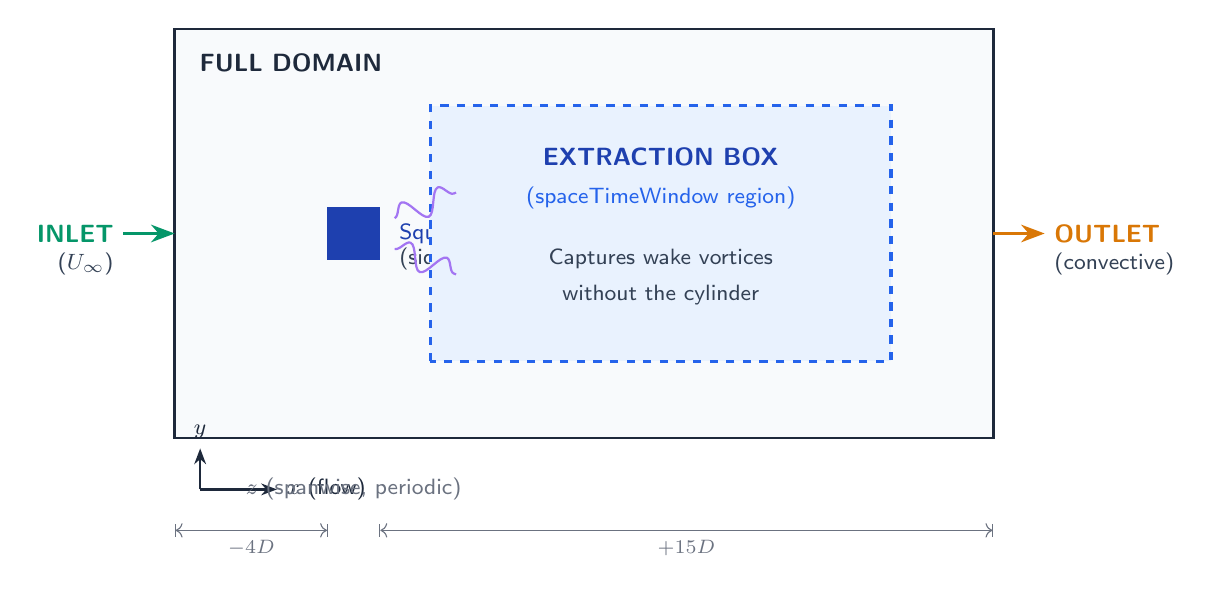
\begin{tikzpicture}[scale=0.65]
    % Full domain outline
    \draw[thick, draw=headingcolor, fill=codebg] (0,0) rectangle (16,8);

    % Domain label
    \node[anchor=north west, font=\small\sffamily\bfseries, color=headingcolor] at (0.3,7.7) {FULL DOMAIN};

    % Square cylinder
    \fill[primarydark] (3,3.5) rectangle (4,4.5);
    \draw[thick, draw=primarydark] (3,3.5) rectangle (4,4.5);
    \node[right, font=\footnotesize\sffamily, color=primarydark] at (4.2,4) {Square cylinder};
    \node[right, font=\footnotesize\sffamily, color=bodytext] at (4.2,3.5) {(side $D$)};

    % Extraction box (dashed, highlighted)
    \fill[primarylight!60] (5,1.5) rectangle (14,6.5);
    \draw[very thick, dashed, primaryblue] (5,1.5) rectangle (14,6.5);

    % Extraction box label
    \node[font=\small\bfseries\sffamily, color=primarydark] at (9.5,5.5) {EXTRACTION BOX};
    \node[font=\footnotesize\sffamily, color=primaryblue] at (9.5,4.7) {(spaceTimeWindow region)};
    \node[font=\footnotesize\sffamily, color=bodytext] at (9.5,3.5) {Captures wake vortices};
    \node[font=\footnotesize\sffamily, color=bodytext] at (9.5,2.8) {without the cylinder};

    % Vortex indication (wavy lines in wake)
    \draw[decorate, decoration={snake, amplitude=1.5mm, segment length=5mm}, accentpurple!70, thick]
        (4.3,4.3) -- (5.5,4.8);
    \draw[decorate, decoration={snake, amplitude=1.5mm, segment length=5mm}, accentpurple!70, thick]
        (4.3,3.7) -- (5.5,3.2);

    % Inlet arrow and label
    \draw[-{Stealth[length=3mm]}, thick, secondarygreen] (-1,4) -- (0,4);
    \node[left, font=\small\sffamily\bfseries, color=secondarygreen] at (-1,4) {INLET};
    \node[left, font=\footnotesize\sffamily, color=bodytext] at (-1,3.4) {($U_\infty$)};

    % Outlet arrow and label
    \draw[-{Stealth[length=3mm]}, thick, warningorange] (16,4) -- (17,4);
    \node[right, font=\small\sffamily\bfseries, color=warningorange] at (17,4) {OUTLET};
    \node[right, font=\footnotesize\sffamily, color=bodytext] at (17,3.4) {(convective)};

    % Coordinate system
    \draw[-{Stealth[length=2mm]}, thick, color=headingcolor] (0.5,-1) -- (2,-1);
    \node[right, font=\footnotesize\sffamily, color=headingcolor] at (2,-1) {$x$ (flow)};
    \draw[-{Stealth[length=2mm]}, thick, color=headingcolor] (0.5,-1) -- (0.5,-0.2);
    \node[above, font=\footnotesize\sffamily, color=headingcolor] at (0.5,-0.2) {$y$};
    \node[font=\footnotesize\sffamily, color=codecomment] at (3.5,-1) {$z$ (spanwise, periodic)};

    % Dimension annotations
    \draw[|<->|, codecomment, thin] (0,-1.8) -- (3,-1.8);
    \node[below, font=\scriptsize\sffamily, color=codecomment] at (1.5,-1.8) {$-4D$};
    \draw[|<->|, codecomment, thin] (4,-1.8) -- (16,-1.8);
    \node[below, font=\scriptsize\sffamily, color=codecomment] at (10,-1.8) {$+15D$};

\end{tikzpicture}
\caption{Computational domain for the square cylinder case showing the extraction box placement in the wake region}
\label{fig:domain}
\end{figure}

\subsection{Extraction Box Placement}

The extraction box is positioned to capture the vortex street while avoiding:

\begin{itemize}
    \item The cylinder itself (to avoid complex geometry in subset)
    \item The inlet region (where flow is uniform and uninteresting)
    \item Domain boundaries (box must be fully internal)
\end{itemize}

Example extraction configuration for this case:

\begin{lstlisting}[language=OpenFOAM,caption={Extraction configuration for square cylinder}]
extractSubset
{
    type            spaceTimeWindowExtract;
    libs            (spaceTimeWindow);

    // Box starts 0.5D downstream of cylinder, extends to 9D
    // Lateral extent captures the wake width
    // Full spanwise extent (periodic direction)
    box             ((0.05 -0.25 0.01) (0.90 0.25 0.38));

    outputDir       "../cylinder-subset";
    fields          (U p nut);
    writeFormat     deltaVarint;

    writeControl    timeStep;
    writeInterval   1;
}
\end{lstlisting}

\subsection{Physical Parameters}

The physical parameters for this case are listed in \cref{tab:cylinder-params}.

\begin{table}[htbp]
\centering
\caption{Square cylinder case parameters}
\label{tab:cylinder-params}
\begin{tabular}{@{}lll@{}}
\toprule
\textbf{Parameter} & \textbf{Value} & \textbf{Description} \\
\midrule
$D$ & 0.04 m & Cylinder side length \\
$U_\infty$ & 8.25 m/s & Freestream velocity \\
$\nu$ & $1.5 \times 10^{-5}$ m$^2$/s & Kinematic viscosity \\
$\text{Re}$ & 21{,}400 & Reynolds number \\
$\text{St}$ & $\approx 0.13$ & Strouhal number \\
$T_{\text{shed}}$ & $\approx 0.037$ s & Vortex shedding period \\
\bottomrule
\end{tabular}
\end{table}

\subsection{Running the Example}

\begin{lstlisting}[language=bash,caption={Running the example case}]
cd examples/ufr2-02

# Generate mesh and run full simulation
./Allrun

# The extraction creates ../ufr2-02-subset with:
#   - Subset mesh in constant/polyMesh
#   - Boundary data in constant/boundaryData
#   - Initial fields

# Initialize and run reconstruction (recommended: inlet-outlet BC)
cd ../ufr2-02-subset
spaceTimeWindowInitCase -sourceCase ../ufr2-02 -inletOutletBC

pimpleFoam

# Alternative: fixed outlet direction for steady-mean flows
# spaceTimeWindowInitCase -sourceCase ../ufr2-02 \
#     -outletDirection "(1 0 0)" \
#     -correctMassFlux
\end{lstlisting}

\subsection{Validation}

The reconstruction can be validated by comparing:

\begin{itemize}
    \item Instantaneous velocity fields at matching timesteps
    \item Vortex shedding frequency (should match original)
    \item Mean velocity profiles in the wake
    \item Reynolds stress components
\end{itemize}

\begin{notebox}
The reconstruction should exactly reproduce the original flow within the extraction region (to solver tolerance) when using exact timestep matching. Small differences may occur at the outlet boundary due to the different boundary condition type.
\end{notebox}

\section{Field Selection by Turbulence Model}
\label{sec:field-selection}

When configuring the extraction, include all fields required by your turbulence model. \Cref{tab:fields-by-model} lists recommended fields for common models.

\begin{table}[htbp]
\centering
\caption{Recommended fields by turbulence model}
\label{tab:fields-by-model}
\begin{tabular}{@{}ll@{}}
\toprule
\textbf{Turbulence Model} & \textbf{Recommended Fields} \\
\midrule
LES Smagorinsky & \texttt{(U p nut)} \\
LES dynamicKEqn & \texttt{(U p nut k)} \\
LES WALE & \texttt{(U p nut)} \\
RANS k-$\varepsilon$ & \texttt{(U p nut k epsilon)} \\
RANS k-$\omega$ SST & \texttt{(U p nut k omega)} \\
Spalart-Allmaras & \texttt{(U p nut nuTilda)} \\
\bottomrule
\end{tabular}
\end{table}

% ----------------------------------------------------------------------------
% REFERENCES
% ----------------------------------------------------------------------------

% For natbib/bibtex:
\bibliography{tutorial}
% For biblatex/biber (comment line above, uncomment below):
% \printbibliography[heading=bibintoc,title={References}]

% ----------------------------------------------------------------------------
% END DOCUMENT
% ----------------------------------------------------------------------------

\end{document}
